\documentclass[10pt,a4paper]{article}
\usepackage{fontspec,amsmath,amssymb,amsthm,mathtools,graphicx,bm,bbm,stmaryrd,nicefrac,mathrsfs}
\usepackage[margin=22mm]{geometry}
\usepackage[bookmarks=false]{hyperref}
\setlength{\emergencystretch}{3em}
\title{Code families on high-dimensional expanders with rate, distance and local-testability guarantees}
\author{Irit Dinur, Siqi Liu, Rachel Yun Zhang}
\date{doi:10.4230/LIPIcs.CCC.2025.27; CC BY 4.0}
\begin{document}
\maketitle
\noindent\textit{Editorial note.} Editable TeX converted from the official CC BY HTML prose and math alttext. Original official PDF/HTML retained. Only the specified claim counts; all author context and available source-local supporting proofs are included.\par\medskip


\par\medskip\noindent\textbf{
1 Introduction}\par




A locally testable code (LTC) is an error correcting code that has a property-tester. The tester reads $q$ bits that are randomly chosen, and rejects words with probability that grows with their distance from the code.\par




LTCs were initially studied and constructed side by side with PCPs (probabilistically checkable proofs). It was only recently that the question of existence of LTCs with the $c^{3}$ property was resolved in the affirmative [6, 31]. A code has the $c^{3}$ property if it has constant rate, constant distance and testable with constant locality.\par




It was initially hoped that high dimensional expanders, a la [25, 24], can serve as the combinatorial structure underlying the code, and all one needs to do is to find an appropriate collection of local codes (at the links) to match up with the combinatorics, see [8, 7, 4].\par




This approach has not borne fruit up until now, essentially due to the stringent requirements on the local codes, which turned out difficult to fulfill. Nevertheless, $c^{3}$ codes were eventually constructed by circumventing the problem and switching from simplicial to square complexes. The main benefit of square complexes is that their local views support tensor codes, which satisfy the requirements for local testability.\par




In this work we return to the simplicial setting and construct a new parameterized family of locally testable codes on simplicial (bounded-degree) high dimensional expanders.
In addition to serving as a new and potentially interesting family of LDPC error-correcting codes, these codes satisfy further properties that could be potentially useful for other applications such as PCPs and beyond. In particular, the codes are symmetric in the sense of [22, 18], meaning that there is a group acting on the coordinates of the codeword, that takes every coordinate to every coordinate. In addition, the fact that local views of our codes are Reed-Solomon, immediately implies that
the codes satisfy the \emph{multiplication property}: the coordinate-wise product of two codewords is a codeword in a related code.\par




These two properties (symmetry and multiplicativity) do not hold for the known constructions of $c^{3}$ LTCs due to their using random linear codes as local codes.\par




Our codes can be described in two seemingly different ways. First, in relation to Reed-Muller codes: our codes are functions on a subset $\bar{X}_{n}\subset\mathbb{F}^{n}$ whose restrictions to a prescribed set of affine lines has low degree. Alternatively, they are Tanner codes on high dimensional expanders, where the coordinates of the codeword correspond to triangles of a $2$-dimensional expander $X$, such that around every edge the local view forms a Reed-Solomon codeword.
The definition of the codes relies on the construction of a specific family of simplicial complexes whose triangles embed naturally into $\mathbb{F}^{n}$, with the property that links of edges embed as affine lines\footnote{An affine line in $\mathbb{F}^{n}$ is given by $\mathbf{a}_{0}\in\mathbb{F}^{n}$ and $\mathbf{a}_{1}\in\mathbb{F}^{n}\setminus\{0\}$ so that $\ell_{e}=\left\{\mathbf{a}_{0}+t\mathbf{a}_{1}\left|\;\vphantom{\mathbf{a}_{0}+t\mathbf{a}_{1}t\in\mathbb{F}}\right.t\in\mathbb{F}\right\}$} in $\mathbb{F}^{n}$.\par



% SOURCE-ID Thmtheorem1


\par\medskip\noindent\textbf{
\textbf{Theorem 1}\textbf{.}
}\par



\emph{Let $\mathbb{F}=\mathbb{F}_{q}$ be a fixed finite field. For every $n$ divisible by $9$ there exists a connected $2$-dimensional $3$-partite simplicial complex $X_{n}$, such that}\par


\begin{enumerate}


\item[] 
(a) 


\emph{For each vertex }$v\in X_{n}(0)$\emph{, the link of }$v$\emph{ is a bipartite }$q$\emph{-regular graph on }$2q^{2}$\emph{ vertices whose normalized adjacency matrix has second largest eigenvalue }$\lambda_{2}=1/\sqrt{q}$\emph{.}\par





\item[] 
(b) 


\emph{There is a set of points }$\bar{X}_{n}\subset\mathbb{F}^{n}$\emph{ and an injective map }$\iota:X_{n}(2)\to\mathbb{F}^{n}$\emph{, such that }$\bar{X}_{n}=Im(\iota)\subset\mathbb{F}^{n}$\emph{, and}\par


\[\begin{gathered}
\lvert X_{n}(2)\rvert=\lvert\bar{X}_{n}\rvert\geq q^{cn}
\end{gathered}\]


\emph{for some absolute constant }$c>0$\emph{.}\par





\item[] 
(c) 


\emph{There is a set }${\cal L}_{n}$\emph{ of affine lines in }$\mathbb{F}^{n}$\emph{ with one line per edge }$e\in X_{n}(1)$\emph{. The line corresponding to an edge }$e$\emph{ is given by a bijection }$\ell_{e}:\mathbb{F}\to{X}_{\scalebox{0.5}{+}e}$\emph{ such that }$\iota\circ\ell_{e}:\mathbb{F}\to\mathbb{F}^{n}$\emph{ is an affine line in }$\mathbb{F}^{n}$\emph{, where we denote }${X}_{\scalebox{0.5}{+}e}=\left\{t\in X_{n}(2)\left|\;\vphantom{t\in X_{n}(2)t\supset e}\right.t\supset e\right\}$\emph{. Let }${\cal L}_{n}=\left\{\iota\circ\ell_{e}\left|\;\vphantom{\iota\circ\ell_{e}e\in
X(1)}\right.e\in X(1)\right\}$\emph{.}\par





\item[] 
(d) 


$X_{n}$\emph{ is }$3$\emph{-partite, so the edges have }$3$\emph{ distinct types and we denote by }${\cal L}^{i}_{n}$\emph{ the set of lines corresponding to type-}$i$\emph{ edges.}\par





\end{enumerate}


\emph{Furthermore, $X_{n}$ and the maps $\iota,\{\ell_{e}\}_{e}$ are constructible in polynomial time in the size of the complex $X_{n}$.}\par



% END-SOURCE-ID Thmtheorem1



The complexes $\{X_{n}\}$ are a slight variant on the coset complexes of [19].
The embedding of $X_{n}(2)$ into $\mathbb{F}^{n}$, so that the links of edges map into affine lines is new, and allows us to define a new family of codes on $X_{n}$,\par



% SOURCE-ID Thmtheorem2


\par\medskip\noindent\textbf{
\textbf{Definition 2}\textbf{ }(HDX local Reed-Solomon Codes)\textbf{.}
}\par



\emph{Let $\mathbb{F}=\mathbb{F}_{q}$ and $\{X_{n}\}_{n}$ be as above, and let $d_{1},d_{2},d_{3}<q$ be positive integers. We define a family of codes as $n\to\infty$,}\par


\[\begin{gathered}
\displaystyle C_{n,d_{1},d_{2},d_{3}} \displaystyle=\left\{f:\bar{X}_{n}\to\mathbb{F}\left|\;\vphantom{f:\bar{X}_{n}\to\mathbb{F}\forall i=1,2,3,\,\forall\ell\in{\cal L}_{n}^{i},\quad f\circ\ell\in RS(q,d_{i})}\right.\forall i=1,2,3,\,\forall\ell\in{\cal L}_{n}^{i},\quad f\circ\ell\in RS(q,d_{i})\right\}
\end{gathered}\]


\emph{where $RS(q,d)\subset\mathbb{F}^{\mathbb{F}}$ is the Reed Solomon code of degree $d$ over $\mathbb{F}$. Note that we have three distinct degree parameters since the edges of the complex have three distinct types.}\par




\emph{The code $C_{n,d_{1},d_{2},d_{3}}$ can alternatively be described as}\par


\[\begin{gathered}
\displaystyle C_{n,d_{1},d_{2},d_{3}} \displaystyle=\left\{f:X_{n}(2)\to\mathbb{F}\left|\;\vphantom{f:X_{n}(2)\to\mathbb{F}\forall e\in X(1),\;f|_{{X}_{\scalebox{0.5}{+}e}}\in C_{e}}\right.\forall e\in X(1),\;f|_{{X}_{\scalebox{0.5}{+}e}}\in C_{e}\right\}.
\end{gathered}\]


\emph{for an appropriate choice of codes $C_{e}\subset\mathbb{F}^{{X}_{\scalebox{0.5}{+}e}}$ such that $C_{e}$ isomorphic to $RS(q,d_{i})$ whenever $e$ is an edge of type $i$.}\par




\emph{We also denote $C_{n,d}=C_{n,d,d,d}$. In the sequel we will often focus on $C_{n,d}$ as it contains all of the ideas, but we wanted to include the slightly more general definition of $C_{n,d_{1},d_{2},d_{3}}$.}\par



% END-SOURCE-ID Thmtheorem2



The isomorphism between definitions (1) and (2) is essentially given by $\iota$ from Theorem 1.
The map $\iota$ identifies $X(2)$ and $\bar{X}_{n}\subset\mathbb{F}^{n}$, and further identifies the set of triangles containing an edge $e\in X(1)$ with an affine line in $\mathbb{F}^{n}$ (see also Section 3.4
and Claim 25 for a full proof).\par




By definition (1) we can see that every $n$-variate polynomial of total degree at most $d=\min(d_{1},d_{2},d_{3})$ gives rise to a codeword in $C_{n,d}$. This allows us to give a non-trivial lower bound on the dimension of $C_{n,d}$ even when $d$ is small and constraint-counting fails. On the other hand, definition (2) allows us to prove distance and local testability through the high dimensional expansion machinery.\par




% SOURCE-ID Thmtheorem3


\par\medskip\noindent\textbf{
\textbf{Theorem 3}\textbf{.}
}\par



\emph{Fix a prime power $q$ and let $d<q$. The family $\{C_{n,d}\}_{n}$ has the following properties}\par


\begin{enumerate}


\item[] 
1. 


\emph{Rate:}\emph{ The dimension of the code is at least the dimension of the Reed-Muller code with }$n/3$\emph{ variables and degree }$d$\emph{. Furthermore, for }$d>\frac{2}{3}q$\emph{ the code has dimension }$\Omega(\lvert X_{n}(2)\rvert)$\emph{ (namely, linear rate as }$n\to\infty$\emph{).}\par





\item[] 
2. 


\emph{Distance:}\emph{ If }$d<q-\Omega(\sqrt{q})$\emph{ the code has constant relative distance }$\Omega_{q}(1)$\emph{.}\par





\item[] 
3. 


\emph{LDPC and Local Testability:}\emph{
For all }$d$\emph{ and }$n$\emph{, the code is defined by parity checks of length }$d+2$\emph{. When }$q$\emph{ is prime, if }$d<q/4$\emph{ the code is locally testable with }$d+2$\emph{ queries.}\par





\item[] 
4. 


\emph{Multiplication:}\emph{ For any }$d_{1},d_{2}$\emph{, and for any }$w_{1}\in C_{n,d_{1}}$\emph{ and }$w_{2}\in C_{n,d_{2}}$\emph{, we have }$w_{1}\odot w_{2}\in C_{n,d_{1}+d_{2}}$\emph{ where }$w_{1}\odot w_{2}$\emph{ is the coordinate-wise product of }$w_{1}$\emph{ and }$w_{2}$\emph{.}\par





\item[] 
5. 


\emph{Symmetric:}\emph{ There is a transitive group action on the coordinates of the code that preserves the code. Transitivity means that for every pair of coordinates }$t,t^{\prime}$\emph{ there is a group element that takes }$t$\emph{ to }$t^{\prime}$\emph{.}\par





\end{enumerate}



% END-SOURCE-ID Thmtheorem3



% SOURCE-ID Thmtheorem4


\par\medskip\noindent\textbf{
$\blacktriangleright$ Remark 4.
}\par



\emph{Here is a table that summarizes the rate, relative distance, and local testability of $\{C_{n,d}\}_{n}$ in different regimes of $d$.}\par









$d$

 


\emph{Rate}

 


\emph{Distance}

 


\emph{Local testability}

 
\par






$(0,q/4)$

 


\emph{$\geq{\binom{n/3}{d}}$}

 


\emph{$\Omega_{q}(1)$}

 


$d+2$

 
\par




$[q/4,\frac{2}{3}q)$

 


\emph{?}

 
\par




$[\frac{2}{3}q,q-\Omega(\sqrt{q}))$

 


$\Omega(\lvert X_{n}(2)\rvert)$

 
\par







\emph{We fail to give a family of $c^{3}$ codes (with constant relative rate, constant relative distance, and local testability with constant number of queries). Specifically, in the low degree regime $d<q/4$, the lower bound on the relative rate is subconstant $>{\binom{n/3}{d}}/\lvert X_{n}(2)\rvert=q^{-\Omega(n)}$. In the high degree regime $d>2q/3$, our approach for showing local testability fails, and we don’t know whether or not local testability occurs.}\par



% END-SOURCE-ID Thmtheorem4



There is a natural way to generalize our complexes and codes to higher dimensions. In Section 6 we describe this generalization and show that distance as well as local testability “trickles down”. We also show that the codes have a homological description as the space of cycles on the top dimension.\par




\par\medskip\noindent\textbf{
1.1 Background}\par




Recent works [6, 31] give locally testable codes that have the $c^{3}$ property, namely they have constant relative rate, constant relative distance and locally testable with a constant number of queries. These codes are constructed on an especially designed squares complex. Similar schemes have been hypothesized to exist on simplicial complexes (see discussion in [6], and see [10]).\par




The simplicial complex codes are defined as\par


\[\begin{gathered}
C=\left\{w\in\mathbb{F}_{q}^{X(2)}\left|\;\vphantom{w\in\mathbb{F}_{q}^{X(2)}w|_{{X}_{\scalebox{0.5}{+}e}}\in C_{e}}\right.w|_{{X}_{\scalebox{0.5}{+}e}}\in C_{e}\right\}
\end{gathered}\]


where we fix, for each edge $e$, a local code $C_{e}\subseteq\mathbb{F}_{q}^{{X}_{\scalebox{0.5}{+}e}}$ where ${X}_{\scalebox{0.5}{+}e}$ is the set of triangles containing the edge $e$. In other words, $C$ is defined by aggregating the local codes $C_{e}$ into one big parity check matrix, using the structure of the HDX. The definition is simple, but the challenge is in analysing properties of $C$ such as rate, distance, or local testability.\par


\begin{enumerate}


\item[] 
1. 


Distance follows quite directly from the distance of each $C_{e}$ together with expansion of $X$.\par





\item[] 
2. 


Local testability can be shown if we manage to show a local version of local testability, per each vertex $v$. Namely, we look at $C_{v}:=C|_{{X}_{\scalebox{0.5}{+}v}}\subseteq\mathbb{F}_{q}^{{X}_{\scalebox{0.5}{+}v}}$, the restriction of the code to the set ${X}_{\scalebox{0.5}{+}v}$ of triangles containing a vertex $v$. This itself is a linear subspace of $\mathbb{F}_{q}^{{X}_{\scalebox{0.5}{+}v}}$. We say that $C_{v}$ itself is locally testable if a good test for $z\stackrel{{\scriptstyle?}}{{\in}}C_{v}$ is to select a random $e\ni v$ and check if $z|_{{X}_{\scalebox{0.5}{+}e}}\in C_{e}$.\par




If each $C_{v}$ is locally testable, then the high dimensional expansion of $X$ would allow us to deduce local testability of the entire code $C$.\par




This is the content of Theorem 41, whose proof is based on the same ideas underlying the proof of local testability in the the squares complex [6, 31] and also earlier the proof of cosystolic expansion in high dimensional expanders [17, 9], and is similar to [10, Proposition 6.4], although there are technical differences.\footnote{They show that if the links are coboundary expanders, then the global sheaf is a cosystolic expander. This is morally equivalent to saying that local robustness implies global local-testability. However, our proof makes use of a weaker local robustness condition, which is what we manage to prove for the local codes.}\par





\item[] 
3. 


The dimension (or rate) of $C$ could a priori be $0$, so one needs to show that $C$ is non-trivial somehow. So far the only successful method has been through constraint counting. One shows that the total number of parity checks is smaller than the number of degrees of freedom. Of course the constraints are often highly dependent so this argument is not tight, and one would like new techniques for lower bounding the dimension.\par





\end{enumerate}


A major difficulty in construction of LTCs is in coming up with a collection of local codes $C_{e}$ that simultaneously allow proving that each $C_{v}$ is locally testable, and at the same time maintain non-trivial dimension for $C$.
Indeed, several prior works gave a general framework for HDX codes but did not know how to instantiate them non-trivially. In [5], the authors gave a definition based on double samplers, and the proof of local testability relies on agreement testing as does ours. In [6], the $c^{3}$ problem has been resolved via a similar approach, but where the underlying complex is a squares complex that has a simpler link structure, which, in turn, implies more flexibility in the choice of local codes. A similar framework is introduced and studied in [10], where codes are described as sections in sheaved high dimensional expanders. All of these works, including the current paper, follow one unifying local to global principle, and are descendants of the work of [17, 9] that showed coboundary expansion based on the same property in the links, plus some form of spectral expansion.\par




In this work we give a first family of codes on high dimensional expanders that are defined by instantiating (3). As mentioned before, our local edge codes $C_{e}$ are Reed-Solomon codes. The codes $C_{v}$ at each vertex turn out to be the following\par


\[\begin{gathered}
C_{v}\cong C_{d_{x},d_{y}}=\left\{f:\mathbb{F}_{q}^{3}\to\mathbb{F}_{q}\left|\;\vphantom{f:\mathbb{F}_{q}^{3}\to\mathbb{F}_{q}\forall a,b,c,\,\,deg_{x}(f(x,b,c))\leq d_{x};\,\,deg_{y}(f(a,y,ay+c))\leq d_{y}}\right.\forall a,b,c,\,\,deg_{x}(f(x,b,c))\leq d_{x};\,\,deg_{y}(f(a,y,ay+c))\leq d_{y}\right\}.
\end{gathered}\]


Quite surprisingly we have learned, after completing this work, that these (local) codes have already been studied in [16], and their rate and distance is known (for the case $d_{x}=d_{y}$). We compute the rate of these codes in the case $d_{x}\not=d_{y}$ for $d_{x}+d_{y}<q/2$ (see Theorem 36), and prove that $C_{d_{x},d_{y}}$ is agreement-testable when $d_{x},d_{y}<q/4$ and when $q$ is a prime (see Theorem 38). Namely, given two functions $X,Y:\mathbb{F}_{q}^{3}\to\mathbb{F}_{q}$ such that
for all $b,c\in\mathbb{F}_{q}$, $X(x,b,c)$ is a low degree function of $x$; and such that for all $a,c\in\mathbb{F}_{q}$, $Y(a,y,ay+c)$ is a low degree function of $y$, if\par


\[\begin{gathered}
\operatorname*{\mathbb{P}}_{a,b,c}[X(a,b,c)\neq Y(a,b,c)]<\epsilon
\end{gathered}\]


then there is some $f\in C_{d_{x},d_{y}}$ that is close to both $X$ and $Y$.
To show that this is a good test we adapt the analysis of Polyschuk and Spielman [32] of the local testability of bivariate polynomial functions. In order to make the analysis go through, we need a characterization of the codewords of the local code, namely that every codeword is described by a polynomial that is low degree in all three coordinate directions. This is given in Lemma 34.
We remark that the local testability we obtain is slightly weaker: there is a quadratic, rather than linear, relation between the distance of the word to a code and the probability of failing the test. Nevertheless we derive local-testability of $C$ from this slightly weaker local testability of the $C_{v}$’s.\par




Finally, as for the dimension of the code $C$. For degree parameters that allow local testability, constraint counting is out of the question, because there are more constraints than degrees of freedom. Instead we show that the code contains many codewords by showing that every low degree multi-variate polynomial is a valid codeword in of our code. We leave for future research to try and get tighter bounds on the rate of these codes.\par




\par\medskip\noindent\textbf{Multiplication Property}\par




A triple $C_{1},C_{2},C_{3}$ of codes are so-called \emph{multiplication codes} if for any $w_{1}\in C_{1}$ and $w_{2}\in C_{2}$ the word $w_{1}\odot w_{2}$ obtained by coordinate-wise product satisfies $w_{1}\odot w_{2}\in C_{3}$. Codes with the multiplication property enable computation “under the hood”, namely, without decoding. Roughly speaking, the product of two codewords is an encoding of the product of the two messages. This can clearly be useful for secure computation. For example, if the two messages represent two subsets, then their product is the intersection of the sets, and we can compute set disjointness without decoding.\par




This property was introduced in [27] who used it towards a proof for $IP=PSPACE$ involving abstract codes, not necessarily Reed-Muller. The original proof of [26, 34] relied on
Reed-Muller codes which are indeed multiplication codes. The multiplication property is used for example in the proof of the PCP theorem [26, 2, 1], and could potentially be useful for constructing PCPs from LTCs.\par




Since our codes are defined as lifts of Reed-Solomon codes they are automatically multiplication codes for appropriate degree choices (a Tanner codes inherits the multiplication property from the local-view codes). Alternatively, they are also
Tanner codes with Reed-Solomon codes as local codes. So these Tanner codes inherit their multiplication property from the local codes. By choosing the parameters appropriately, we can get $C_{1},C_{3}$ an LDPC code with linear rate, and $C_{2}$ a locally testable (LDPC) code with polynomial rate, such that this triple has the multiplication property (see Lemma 27).\par





\par\medskip\noindent\textbf{Connection to Reed-Muller codes, lifted codes, and Tanner Codes}\par




Recall that a Tanner code is given by two pieces of data:\par


\begin{itemize}


\item[] 
$\blacksquare$ 


A bipartite graph ${\cal G}=({\cal B},{\cal P},E)$ with left vertices ${\cal B}$ (for bits), right vertices ${\cal P}$ (for parity checks), and edges $E$.\par





\item[] 
$\blacksquare$ 


For each $p\in{\cal P}$ there is a local code $C_{p}\subset\mathbb{F}^{\Gamma(p)}$ where $\Gamma(p)\subset{\cal B}$ are the neighbors of $p$.\par





\end{itemize}


Given ${\cal G}$ and $\{C_{p}\}$, the Tanner code is\par


\[\begin{gathered}
{\cal T}({\cal G},\{C_{p}\})=\left\{w\in\mathbb{F}^{\cal B}\left|\;\vphantom{w\in\mathbb{F}^{\cal B}\forall p\in{\cal P},\;w|_{\Gamma(p)}\in C_{p}}\right.\forall p\in{\cal P},\;w|_{\Gamma(p)}\in C_{p}\right\}.
\end{gathered}\]




The Reed-Muller code $RM_{n,d}$ is the space of all $n$-variate polynomials of total degree at most $d$.
For a broad set of parameters, Reed-Muller codes are themselves known to be Tanner codes, with local parity check codes being Reed Solomon codes, and with a ${\cal B}=\mathbb{F}^{n}$ and ${\cal P}$ being the set of all affine lines in $\mathbb{F}^{n}$, so that the bipartite graph ${\cal G}_{RM}$ is the point-vs.-line graph which connects a point in $\mathbb{F}^{n}$ to all lines passing through it.
For some parameter regimes (when the degree is high) such Tanner codes form a larger space than the Reed-Muller codes, as was discovered and studied in [14], where such codes are termed “lifted codes”.
Later in [11], partial lifts are considered where some of the vertices of ${\cal P}$ are erased and one considers the remaining punctured code. Clearly, different choices of where to puncture will have different properties. The codes studied in [11] are locally correctable and each point in $\mathbb{F}^{n}$ is contained in $\mathrm{poly}(n)$ affine lines in ${\cal P}$.
This type of codes resembles the situation in our codes, as we explain next, but a key difference is that in our construction each point in $\mathbb{F}^{n}$ only participates in constant number of parity checks.\par




The code $C_{n,d_{1},d_{2},d_{3}}$, as per (1), can be viewed a Tanner code whose graph is a subgraph of ${\cal G}_{RM}$ obtained by keeping a subset ${\cal L}_{n}$ of the lines, and a subset $\bar{X}_{n}\subset\mathbb{F}^{n}$ of the points. We also allow different degree restrictions on different types of lines. If we set $d=d_{1}=d_{2}=d_{3}$ the parity check matrix of $C_{n,d}$ is thus a sub-matrix of the parity check matrix of the Reed-Muller code matrix.
As for (2), it can be seen as a Tanner code on the bipartite graph ${\cal G}=(X(2),X(1),E)$ connecting each edge $e\in X(1)$ on the right to the set ${X}_{\scalebox{0.5}{+}e}\subset X(2)$ of triangles containing it, and putting a Reed-Solomon code on every ${X}_{\scalebox{0.5}{+}e}$ in a specified way.\par





\par\medskip\noindent\textbf{Two-query testability}\par




One can often convert a code that is testable with $q$ queries to another code that is testable with two queries, while increasing the alphabet. This is done by converting each codeword to the list of its local views. For example, in the case of Reed-Muller codes, instead of representing a polynomial by its evaluation on points, we represent it by providing its restriction to each plane. This is sometimes called the planes table, and is two-query testable by the plane-vs.-plane test, see [33]. In the case of $c^{3}$ LTCs of [6, 31], this conversion is immediate, although it is not described there explicitly. For our codes it also holds, and we include details in Claim 17. This property was also highlighted in [10].\par






\par\medskip\noindent\textbf{
1.2 Further Work}\par




This work raises many questions for further investigation.\par


\begin{itemize}


\item[] 
$\blacksquare$ 


\textbf{Better bounds.} What is the exact rate of our codes? We give a lower bound based on Reed-Muller codes, but we don’t know how close this bound is to the truth. Are there parameter regimes where our codes are $c^{3}$?\par





\item[] 
$\blacksquare$ 


\textbf{Efficient encoding.} Our codes are specified by their parity-check matrices. A generator matrix can be computed in $O(N^{3})$ time, where $N$ is the block length. Given the generator matrix, computing an encoding takes time $O(N^{2})$. Can encoding be done more efficiently, ideally even in linear-time?\par





\item[] 
$\blacksquare$ 


\textbf{Quantum codes.} It has recently become clear that locally testable HDX codes are related to quantum LDPC codes of the CSS type. Our construction gives a $2$-chain (from vertices to edges to triangles) which can automatically be viewed as a quantum LDPC code. Indeed, we show in Section 2.6 how any HDX code gives rise to a sheaf which, by [10, Section 7.4], gives rise to a quantum code. Our local testability analysis implies distance in one direction, whereas for a good quantum LDPC code, one needs to prove both distance as well as co-distance. This is an interesting challenge. Moreover, in Section 6 we show how our construction generalizes to $k$ dimensions, which, by the same recipe as above, can be converted to a sheaf and a $k+1$-chain. Studying the resulting quantum codes at intermediate levels $0<i<k$ seems like an interesting direction.\par





\item[] 
$\blacksquare$ 


\textbf{Sparsified Grassmannian.} We have constructed a collection of affine lines with the property that each point has exactly three lines passing through it. This is a very sparse collection of lines, that never-the-less expands quite well when we walk from point to line to point. How does this generalize to higher dimensional complexes? The question of finding sparse Grassmannians has been studied in [29, 3, 21, 13] and could provide new PCP gadgets with properties similar to [23].\par





\item[] 
$\blacksquare$ 


\textbf{Other coset complexes.} We have considered a variant of the coset complexes of Kaufman and Oppenheim, by choosing subgroups based on a sub-ring of the ring chosen in [19]. Many high dimensional expanders are based on matrix groups [25, 24, 19, 30]. Thus similar embeddings of the complexes into $\mathbb{F}^{n}$ could potentially be useful for coming up with new codes, whose properties can be studied through the high dimensional expansion framework.\par





\item[] 
$\blacksquare$ 


\textbf{Generalized sumcheck.} Many interactive proof systems reduce proving certain relations to checking that a multi-variate polynomial $p(x_{1},\dots,x_{m})$ over $\mathbb{F}^{m}$ sums up to zero over some subset $\mathbb{H}^{m}\subseteq\mathbb{F}^{m}$. The sumcheck protocol is designed to check this relation by recursively restricting variables of $p$ and checking the condition over smaller sets of random variables.
Can one design sumcheck-like protocols for codes other than Reed-Muller? For example, in the case of our code, we would need to find subsets of points that play the role of $H^{m}$, so that one can test whether some partial sums of a codeword sum up to zero.\par




Perhaps a first step would be to find a sumcheck protocol for our local codes $C_{d_{x},d_{y}}$.\par





\end{itemize}





\par\medskip\noindent\textbf{
1.3 Organization}\par




We define our coset complex in Section 3 and prove its properties (Theorem 1) in Sections 3.1, 3.2, and 3.3. We then define our code on this coset complex in Section 3.4. Its properties as detailed in Theorem 3 are proved in the following sections:\par


\begin{itemize}


\item[] 
$\blacksquare$ 


In Section 3.5 we show that our code has the multiplication property, and in Section 3.6, we show that our code has constant distance in appropriate parameter regimes (items 2 and 4 of Theorem 3). We also show that our code has the transivity property (item 5).\par





\item[] 
$\blacksquare$ 


We discuss the rate (item 1) of the global and local codes in Sections 4.1 and 4.2 respectively.\par





\item[] 
$\blacksquare$ 


In Sections 5.1 and 5.3, we prove that the local and global codes are agreement testable.\par





\end{itemize}


Finally, in Section 6 we describe the generalization to higher dimensions.\par






\par\medskip\noindent\textbf{
2 Preliminaries}\par




\par\medskip\noindent\textbf{
2.1 Expander Graphs}\par




A $d$-regular graph $G$ is said to be a $\gamma$-one-sided expander if it has eigenvalues $d=\lambda_{1}\geq\lambda_{2}\geq...\geq\lambda_{n}\geq-d$ which satisfy $\lambda_{i}\leq\gamma\cdot d$ for all $i>1$.\par



% SOURCE-ID Thmtheorem5


\par\medskip\noindent\textbf{
\textbf{Lemma 5}\textbf{ }(Alon-Chung)\textbf{.}
}\par



\emph{Let $G=(V,E)$ be a $d$-regular $\gamma$ one-sided expander. Let $T\subseteq V$ be such that the graph induced on $T$ has average degree at least $\delta d$. Then $|T|\geq(\delta-\gamma)\cdot|V|$.}\par



% END-SOURCE-ID Thmtheorem5



\par\medskip\noindent\textbf{Proof.}\par




Let $A$ be the normalized adjacency matrix of $G$ and let $f$ be the indicator function of $T$. Using the spectral decomposition $f=\frac{|T|}{|V|}{\mathbf{1}}+f^{\perp}$ we get\par


\[\begin{gathered}
\delta d|T|\leq 2E(T)=f^{\top}Af\leq\lvert T\rvert^{2}d/|V|+\gamma d\lvert T\rvert
\end{gathered}\]


where $E(T)$ denotes the number of edges in the induced graph on $T$.
Dividing both sides by $d|T|$ and rearranging gives the lemma.
$\blacktriangleleft$\par






\par\medskip\noindent\textbf{
2.2 High Dimensional Expanders}\par




A pure $k$-dimensional simplicial complex $X$ is a set system (or hypergraph) consisting of a set of vertices $X(0)$ and an arbitrary collection of subsets of size $k+1$ together with all their subsets. The sets of size $i+1$ in $X$ are denoted by $X(i)$. We will sometimes omit set brackets and write for example $uvw\in X(2)$ instead of $\{u,v,w\}\in X(2)$. As convention $X(-1)=\{\emptyset\}$. Unless it is otherwise stated, we always assume that $X$ is finite.\par




Let $i<k$ and $s\in X(i)$. It is standard to define the link of $s$ to be a $k-i-1$-dimensional simplicial complex defined by
$X_{s}=\left\{t\setminus s\left|\;\vphantom{t\setminus st\in X,t\supseteq s}\right.t\in X,t\supseteq s\right\}$. We also define the less-standard but useful notation\par



% SOURCE-ID Thmtheorem6


\par\medskip\noindent\textbf{
\textbf{Definition 6}\textbf{ }(Star)\textbf{.}
}\par



\emph{For a $k$-dimensional complex $X$ and a face $s\in X(i)$ for some $i<k$, the star of $s$ is the $k$-dimensional complex containing all faces that contain $s$.}\par


\[\begin{gathered}
{X}_{\scalebox{0.5}{+}s}(j)=\left\{t\in X(j)\left|\;\vphantom{t\in X(j)t\supseteq s}\right.t\supseteq s\right\}.
\end{gathered}\]



% END-SOURCE-ID Thmtheorem6



For a face $s\in X(i)$, there is a natural bijection ${X}_{\scalebox{0.5}{+}s}(j)\to X_{s}(j-i-1)$ mapping $t\in{X}_{\scalebox{0.5}{+}s}$ to $t\setminus s\in X_{s}$.\par



% SOURCE-ID Thmtheorem7


\par\medskip\noindent\textbf{
\textbf{Definition 7}\textbf{ }(High dimensional link expander)\textbf{.}
}\par



\emph{Let $X$ be a $k$-dimensional simplicial complex. Let $\lambda\geq 0$. We say that $X$ is a one-sided $\lambda$-link expander if for every $s\in X^{\leq k-2}$, the graph $(X_{s}(0),X_{s}(1))$ is a $\lambda$-one sided spectral expansion.}\par



% END-SOURCE-ID Thmtheorem7


% SOURCE-ID Thmtheorem8


\par\medskip\noindent\textbf{
\textbf{Definition 8}\textbf{ }(Coset complex)\textbf{.}
}\par



\emph{A $k$-dimensional coset complex is given by a group $G$ and subgroups $K_{1},\ldots,K_{k+1}$. The vertices are all cosets of the $k+1$ subgroups, and the $i$-faces are all $i+1$-tuples of cosets that have a non-empty intersection. The complex is denoted
$X[G;K_{1},\ldots,K_{k+1}]$.}\par



% END-SOURCE-ID Thmtheorem8



The degree of a complex is defined as $\max_{v\in X(0)}\lvert\left\{e\in X(1)\left|\;\vphantom{e\in X(1)v\subset e}\right.v\subset e\right\}\rvert$, the maximum edge degree of a vertex. A beautiful construction of a constant-degree coset complex that is a high dimensional expander was given in [19], see also [15, 30].\par




It is not hard to see that links in a coset complex are themselves coset complexes.\par





\par\medskip\noindent\textbf{
2.3 Random Walks on High Dimensional Expanders}\par




Let $X$ be a regular two-dimensional complex, so that every vertex touches the same number edges, and every edge touches the same number of triangles. This assumption is not needed, but it is satisfied by our coset complexes and it slightly simplifies the definitions below.\par




Let $V=X(0),E=X(1),{X}_{\scalebox{0.5}{+}}=X(2)$, and also denote $X(-1)=\{\phi\}$.\par




The down operator $D^{i}:\mathbb{R}^{X(i)}\to\mathbb{R}^{X(i-1)}$ (for $0\leq i\leq 2$) and the up operator $U^{i}:\mathbb{R}^{X(i)}\to\mathbb{R}^{X(i+1)}$ (for $-1\leq i\leq 1$) are defined by\par


\[\begin{gathered}
\displaystyle\forall a\in X(i-1),\quad D^{i}f(a) \displaystyle=\operatorname*{\mathbb{E}}_{b\supset a}[f(b)], \\
\displaystyle\forall b\in X(i+1),\quad U^{i}g(b) \displaystyle=\operatorname*{\mathbb{E}}_{a\subset b}[g(a)].
\end{gathered}\]


We will often drop the superscript $i$ in $U^{i}$ and $D^{i}$ when it is clear what $i$ is.\par




Let $e\smallsmile e^{\prime}$ denote the lower random walk on the edges (choose a random $e$, then $v\in e$, then $e^{\prime}\ni v$). It is easy to see that the Markov operator corresponding to this walk is just $UD$.
Let $e\smallfrown e^{\prime}$ denote the non-lazy upper random walk on the edges (choose a random $e$, then $t\supset e$, then $e^{\prime}\in t$ such that $e^{\prime}\neq e$). It is not hard to see that the Markov operator corresponding to this walk, denoted $M^{+}$, satisfies $DU=\frac{2}{3}M^{+}+\frac{1}{3}I$.\par




We define inner products on the spaces $\mathbb{R}^{V},\mathbb{R}^{E}$ by expectation according to the uniform distribution (here we are using the regularity assumption).\par




For example, for $f,g:V\to\mathbb{R}$\par


\[\begin{gathered}
\langle f,g\rangle=\operatorname*{\mathbb{E}}_{x\in V}[f(x)g(x)],\qquad\lVert f\rVert=(\langle f,f\rangle)^{1/2}.
\end{gathered}\]


The following is by now well known, see [8, 20], and we include a proof for completeness.\par



% SOURCE-ID Thmtheorem9


\par\medskip\noindent\textbf{
\textbf{Lemma 9}\textbf{.}
}\par



\emph{Let $X$ be a one-sided $\gamma$-link expander. Every $g\in\mathbb{R}^{E}$ satisfies}\par


\[\begin{gathered}
\langle g,M^{+}g\rangle\leq\langle g,(UD+\gamma I)g\rangle.
\end{gathered}\]



% END-SOURCE-ID Thmtheorem9



In particular, for a set $R\subset X(1)$ such that $\beta=\operatorname*{\mathbb{P}}_{e\smallfrown e^{\prime}}[e\in R|e^{\prime}\in R]$ it must be that\par


\[\begin{gathered}
\operatorname*{\mathbb{P}}_{e\smallsmile e^{\prime}}[e\in R|e^{\prime}\in R]\geq\beta-\gamma
\end{gathered}\]


by applying the lemma on $g={\mathbf{1}}_{R}$ and observing that $\operatorname*{\mathbb{P}}_{t\in X(2),e\neq e^{\prime}\subset t}[e,e^{\prime}\in R]=\beta\operatorname*{\mathbb{P}}[R]$.\par




\par\medskip\noindent\textbf{Proof.}\par




\[\begin{gathered}
\displaystyle\langle g,M^{+}g\rangle \displaystyle=\operatorname*{\mathbb{E}}_{abc\in{X}_{\scalebox{0.5}{+}}}g(ab)g(ac) \\
\displaystyle=\operatorname*{\mathbb{E}}_{a}\operatorname*{\mathbb{E}}_{bc\in X_{a}(1)}[g(ab)g(ac)] \\
\displaystyle\leq\operatorname*{\mathbb{E}}_{a}\operatorname*{\mathbb{E}}_{b,c\in X_{a}(0)}[g(ab)g(ac)]+\gamma\operatorname*{\mathbb{E}}_{a}\operatorname*{\mathbb{E}}_{b\in X_{a}(0)}[g(ab)^{2}] \\
\displaystyle=\langle g,UDg\rangle+\gamma\lVert g\rVert^{2}
\end{gathered}\]


where the inequality follows since $X_{a}$ is a $\gamma$-one-sided expander for each $a$, and this means that for any $f:X_{a}(0)\to\mathbb{R}$ (and in particular setting $f(b):=g(ab)$),\par


\[\begin{gathered}
\operatorname*{\mathbb{E}}_{bc\in X_{a}(1)}f(b)f(c)\leq\operatorname*{\mathbb{E}}_{b,c\in X_{a}(0)}f(b)f(c)+\gamma\cdot\operatorname*{\mathbb{E}}_{b\in X_{a}(0)}f(b)^{2}.
\end{gathered}\]


Note that the distribution of choosing $a$ and then two edges $ab,ac$ independently, is equivalent to choosing a random edge $e^{\prime}$, then a random vertex $a\in e^{\prime}$ and then another edge $e\ni a$.
$\blacktriangleleft$
The following swap walk $S_{0,1}$ that starts from a random edge in $X(1)$ and ends at some vertex in $X(0)$ will be used in the analysis of local testability of the global code. Starting with a random edge $e$, choose a random triangle $t\ni e$ and output $v=t\setminus e$.\par



% SOURCE-ID Thmtheorem10


\par\medskip\noindent\textbf{
\textbf{Lemma 10}\textbf{.}
}\par



\emph{Let $X$ be a two-dimensional $\gamma$-link-expander. The random walk $\tilde{M}=S_{0,1}D$ on the edges has second largest eigenvalue bounded by $3\gamma$.}\par



% END-SOURCE-ID Thmtheorem10




\par\medskip\noindent\textbf{Proof.}\par




We claim that\par


\[\begin{gathered}
M^{+}UD=\frac{1}{2}S_{0,1}D+\frac{1}{2}UD.
\end{gathered}\]


Let us analyze the random walk corresponding to the operator $M^{+}UD$. We note that when viewed as an operator for functions in $\mathbb{R}^{E}$,\par


\[\begin{gathered}
M^{+}UDf(e)=\operatorname*{\mathbb{E}}_{e_{1}\stackrel{{\scriptstyle M^{+}}}{{\sim}}e}[UDf(e_{1})]=\operatorname*{\mathbb{E}}_{e^{\prime}\stackrel{{\scriptstyle UD}}{{\sim}}e_{1}\stackrel{{\scriptstyle M^{+}}}{{\sim}}e}[f(e^{\prime})].
\end{gathered}\]


The underlying random walk from $e$ to $e^{\prime}$ is as follows.
We start from an edge $e$, go (via $M^{+}$) to a random edge $e_{1}$ such that $e\cup e_{1}\in X(2)$. We then
go from $e_{1}$, via $UD$, to an edge $e^{\prime}$. In this step two things can happen, each with probability $1/2$. Either $e^{\prime}$ doesn’t contain $\{v\}=e_{1}\cap e$, in which case we end up with the distribution of $S_{0,1}D$; or $e^{\prime}\ni v$, in which case we end up with $UD$. This proves the required equality.
We can thus write $S_{0,1}D=2M^{+}UD-UD$. Furthermore, by Lemma 9 we have that for any $f\in\mathbb{R}^{E}$,\par


\[\begin{gathered}
\langle f,(2M^{+}UD-UD)f\rangle\leq\langle f,(2(UDUD+\gamma UD)-UD)f\rangle.
\end{gathered}\]


So for any $f\in\mathbb{R}^{E}$ with $\operatorname*{\mathbb{E}}[f]=0$ we get,\par


\[\begin{gathered}
\langle f,S_{0,1}Df\rangle\leq\langle f,(2UDUD-UD)f\rangle+2\gamma\lVert f\rVert^{2}=\langle f,U(2DU-I)Df\rangle+2\gamma\lVert f\rVert^{2}\leq 3\gamma\lVert f\rVert^{2}
\end{gathered}\]


where in the last inequality we have used the fact that $2DU-I$ is nothing other than the random walk from vertex to vertex in the graph $(X(0),X(1))$, so by assumption on $X$, $\langle(2DU-I)g,g\rangle\leq\gamma\lVert g\rVert^{2}$ for every function $g\in\mathbb{R}^{V}$ such that $\operatorname*{\mathbb{E}}[g]=0$.
$\blacktriangleleft$\par






\par\medskip\noindent\textbf{
2.4 HDX Codes}\par




An HDX code is defined by two objects\par


\begin{itemize}


\item[] 
$\blacksquare$ 


A $k$-dimensional simplicial complex $X$, and a dimension $0<i\leq k$.\par





\item[] 
$\blacksquare$ 


A collection $\{C_{s}\}$ of local codes $C_{s}\subseteq\mathbb{F}_{q}^{{X}_{\scalebox{0.5}{+}s}(k)}$, one per face $s\in X(k-i)$.\par





\end{itemize}


The HDX code at dimension $k$ is defined as\par


\[\begin{gathered}
{\cal C}^{k}[X,\{C_{s}\}]=\left\{f\in\mathbb{F}_{q}^{X(k)}\left|\;\vphantom{f\in\mathbb{F}_{q}^{X(k)}\forall s\in X(k-i),\;(\;f(s\cup v):v\in X_{s}(i-1)\;)\in C_{s}}\right.\forall s\in X(k-i),\;(\;f(s\cup v):v\in X_{s}(i-1)\;)\in C_{s}\right\}
\end{gathered}\]


When $X$ is one dimensional these are the expander codes of [35].\par




\par\medskip\noindent\textbf{Example 1: expander code}\par




An expander code is given by an expander graph $X=(V,E)$ and a local code $C_{v}$ for every vertex $v\in V$ such that $C_{v}\subseteq\mathbb{F}_{2}^{\{e\ni v\}}$. A word $f\in\mathbb{F}_{2}^{E}$ is in the code if for every vertex $v$, the bits on the edges touching $v$ form a codeword in a small code $C_{v}$. Formally, if $(f(e):e\ni v)\in C_{v}$. Often the graph $(V,E)$ is $d$-regular and the local codes are taken to all be copies of some $C_{0}\subset\mathbb{F}_{2}^{d}$.\par




This is a special case of (5) for dimension $k=1$, where $X(0)=V$ and $X(1)=E$ and $C_{v}\subseteq\mathbb{F}_{2}^{X_{v}(0)}$ via the identification $X_{v}(0)\leftrightarrow\{e\ni v\}$.\par





\par\medskip\noindent\textbf{Example 2: cocycle codes}\par




Fix some simplicial complex $X$, and some dimension $0<k<dim(X)$. Suppose for every $s\in X(k-1)$, the local code $C_{s}$ is taken to be the parity code consisting of all even length words, namely the local code at $s\in X(k-1)$ is,\par


\[\begin{gathered}
Z_{s}=\left\{f\in\mathbb{F}_{2}^{X_{s}(0)}\left|\;\vphantom{f\in\mathbb{F}_{2}^{X_{s}(0)}\sum_{v\in X_{s}(0)}f(s\cup v)=0}\right.\sum_{v\in X_{s}(0)}f(s\cup
v)=0\right\}.
\end{gathered}\]


Then the $k$ dimensional HDX code $C[X,\{Z_{s}\}]$ coincides with the space of $k$-cocycles of $X$. For example, when $k=1$, the code is spanned by all closed walks.\par






\par\medskip\noindent\textbf{
2.5 Local-Testability and Agreement-Testability}\par




For a function $f:A\to B$ and a subset $A^{\prime}\subset A$ we denote by $f|_{A^{\prime}}:A^{\prime}\to B$ the restriction of $f$ to $A^{\prime}$.\par




Let $X$ be a $k$-dimensional simplicial complex and assume that for every $v\in X(0)$ we are given a local code $C_{v}\subseteq\mathbb{F}_{q}^{{X}_{\scalebox{0.5}{+}v}}$. Let $C={\cal C}^{k}[X,\{C_{v}\}]\subseteq\mathbb{F}_{q}^{X(k)}$ be an HDX code.\par



% SOURCE-ID Thmtheorem11


\par\medskip\noindent\textbf{
\textbf{Definition 11}\textbf{ }(Locally testable code)\textbf{.}
}\par



\emph{Let $\rho:\mathbb{R}_{+}\to\mathbb{R}_{+}$ be a strictly increasing function with $\rho(0)=0$, and let $\epsilon>0$. A code $C\subseteq\mathbb{F}_{q}^{n}$ is a $(Q,\epsilon,\rho(\cdot))$-locally testable code if there is a randomized tester that, upon receiving a given word $f\in\mathbb{F}_{q}^{n}$, queries $f$ in at most $Q$ locations and then accepts or rejects, such that
if $p=\operatorname*{\mathbb{P}}[\hbox{Tester rejects }f]\leq\epsilon$ then $\operatorname{dist}(f,C)\leq\rho(p)$.}\par



% END-SOURCE-ID Thmtheorem11



We specialize this definition to the case of HDX codes by considering a “cannonical” local tester that selects a random vertex $v$ and checks if the restriction of the codeword to the star of $v$ is in the local code $C_{v}$. Namely, if $f|_{{X}_{\scalebox{0.5}{+}v}}\in C_{v}$. The number of queries made by this tester is equal to the maximal number of $k$-faces containing a vertex $v$.\par



% SOURCE-ID Thmtheorem12


\par\medskip\noindent\textbf{
\textbf{Definition 12}\textbf{ }(Local testability of HDX Codes)\textbf{.}
}\par



\emph{Let $\rho:\mathbb{R}_{+}\to\mathbb{R}_{+}$ be a strictly increasing function with $\rho(0)=0$, and let $\epsilon>0$.
The HDX code $C={\cal C}^{k}[X,\{C_{v}\}]$ is
$(\epsilon,\rho(\cdot))$-locally testable if for any $f\in\mathbb{F}_{q}^{X(k)}$, denoting $p=\operatorname*{\mathbb{P}}_{v}[f|_{{X}_{\scalebox{0.5}{+}v}}\not\in C_{v}]$, the following holds. If $p\leq\epsilon$ then}\par


\[\begin{gathered}
\operatorname{dist}(f,C)\leq\rho(p).
\end{gathered}\]



% END-SOURCE-ID Thmtheorem12


% SOURCE-ID Thmtheorem13


\par\medskip\noindent\textbf{
$\blacktriangleright$ Remark 13.
}\par



\emph{If an HDX code is locally testable as per Definition 12, then the number of queries made by the tester is at most $\max_{v}|X_{+v}(k)|$ which is the maximal number of $k$-faces containing a vertex $v$. In a bounded-degree complex $X$ this is a constant number.
Moreover, if each $C_{v}$ is an LDPC, we can reduce the query complexity further (without changing the code), as in the following Claim.}\par



% END-SOURCE-ID Thmtheorem13


% SOURCE-ID Thmtheorem14


\par\medskip\noindent\textbf{
Claim 14. 
}\par



Suppose each local code $C_{v}$ is defined by at most $m_{0}$ parity checks, each looking at most $q_{0}$ bits. If an HDX code ${\cal C}^{k}[X,\{C_{v}\}]$ is $(\epsilon,\rho(\cdot))$-locally testable per Definition 12, then it is $(q_{0},\frac{\epsilon}{m_{0}},\rho^{\prime}(\cdot))$-locally testable as per Definition 11, where $\rho^{\prime}(x):=\rho(m_{0}x)$.\par



% END-SOURCE-ID Thmtheorem14



\par\medskip\noindent\textbf{
\textbf{Proof}.}\par




For any vertex $v$, $f|_{{X}_{\scalebox{0.5}{+}v}}\in C_{v}$ iff none of the $m_{0}$ parity checks fail. By union bound, the fraction of vertices $v$ for which at least one of the $m_{0}$ parity checks fail is at most $m_{0}\cdot\frac{\epsilon}{m_{0}}=\epsilon$. This means that $\operatorname*{\mathbb{P}}_{v}[f|_{{X}_{\scalebox{0.5}{+}v}}\not\in C_{v}]\leq
m_{0}p<\epsilon$, and by the local testability per Definition 12 we deduce that $\operatorname{dist}(f,C)\leq\rho(m_{0}p)$.
$\vartriangleleft$\par



% SOURCE-ID Thmtheorem15


\par\medskip\noindent\textbf{
\textbf{Definition 15}\textbf{ }(Agreement testability of HDX Codes)\textbf{.}
}\par



\emph{Let $\rho:\mathbb{R}_{+}\to\mathbb{R}_{+}$ be a strictly increasing function, and let $\epsilon>0$.
The HDX code ${\cal C}^{k}[X,\{C_{v}\}]$ is called $(\epsilon,\rho(\cdot))$-agreement testable if, for any given collection $\left\{z_{v}\in C_{v}\left|\;\vphantom{z_{v}\in C_{v}v\in X(0)}\right.v\in X(0)\right\}$, if}\par


\[\begin{gathered}
\alpha:=\operatorname*{\mathbb{P}}_{uv\in X(1)}[z_{v}({X}_{\scalebox{0.5}{+}uv}(k))\neq z_{u}({X}_{\scalebox{0.5}{+}uv}(k))]<\epsilon
\end{gathered}\]


\emph{then there exists some $h\in C$ such that}\par


\[\begin{gathered}
\operatorname*{\mathbb{P}}_{v\in X(0)}(z_{v}\neq h|_{{X}_{\scalebox{0.5}{+}v}(k)})\leq\rho(\alpha).
\end{gathered}\]



% END-SOURCE-ID Thmtheorem15


% SOURCE-ID Thmtheorem16


\par\medskip\noindent\textbf{
Claim 16 (Agreement testability implies local testability). 
}\par



Let $X$ be a $k$-dimensional simplicial complex, and assume that every vertex is contained in the same number of $k$ faces. Let $C={\cal C}^{k}[X,\{C_{v}\}]$ be an HDX code.
If $C$ is $(\epsilon_{0},\rho_{0}(\cdot))$-agreement testable then it is $(\epsilon_{0}/2,\rho_{1}(\cdot))$-locally testable, where $\rho_{1}(p):=\rho_{0}(2p)+p$.\par



% END-SOURCE-ID Thmtheorem16




\par\medskip\noindent\textbf{
\textbf{Proof}.}\par




Suppose $f\in\mathbb{F}_{q}^{X(k)}$.
Assume that $p=\operatorname*{\mathbb{P}}_{v}[f|_{{X}_{\scalebox{0.5}{+}v}}\not\in C_{v}]$. Let $V^{*}=\left\{v\in X(0)\left|\;\vphantom{v\in X(0)f|_{{X}_{\scalebox{0.5}{+}v}}\in C_{v}}\right.f|_{{X}_{\scalebox{0.5}{+}v}}\in C_{v}\right\}$. Set $z_{v}=\begin{cases}f|_{{X}_{\scalebox{0.5}{+}v}}&v\in V^{*}\\
0&v\not\in V^{*}\end{cases}$.
Choose a random edge $uv\in X(1)$. The probability that either $u$ or $v$ are not in $V^{*}$ is at most $2p$. In the remaining probability they surely agree, so the disagreement is at most $\alpha\leq 2p$.
If $2p\leq\epsilon_{0}$, then by the assumption on agreement testability, there must be some codeword $h\in C$ such that
$\operatorname*{\mathbb{P}}_{v}[z_{v}\neq h|_{{X}_{\scalebox{0.5}{+}v}}]\leq\rho_{0}(\alpha)\leq\rho_{0}(2p)$.
The codeword $h$ disagrees with $f$ on some ${X}_{\scalebox{0.5}{+}v}$ either when $v\not\in V^{*}$ or when $z_{v}\neq h|_{{X}_{\scalebox{0.5}{+}v}}$. This event is upper bounded by $p+\rho_{0}(2p)=\rho_{1}(p)$. By assumption every vertex is contained in the same number of $k$-faces. So choosing a random vertex and then a random $k$-face containing it, is the same as choosing a random $k$-face. Therefore,\par


\[\begin{gathered}
\operatorname{dist}(f,C)\leq\operatorname{dist}(f,h)=\operatorname*{\mathbb{P}}_{s\in X(k)}[f(s)\neq h(s)]\leq\operatorname*{\mathbb{P}}_{v\in X(0)}[v\not\in V^{*}]+\operatorname*{\mathbb{P}}_{v\in X(0)}[z_{v}\neq h|_{{X}_{\scalebox{0.5}{+}v}}]\leq\rho_{1}(p).
\end{gathered}\]


$\vartriangleleft$\par




Since there has been some discussion of this in the literature [10], we spell out how any HDX code that is agreement testable automatically gives rise to the “local-view” code that is two-query testable. The idea is to move from a codeword $f\in C$ to the collection $\{z_{v}\}_{v\in X(0)}$ of local views where $z_{v}=f|_{{X}_{\scalebox{0.5}{+}v}}$.\par



% SOURCE-ID Thmtheorem17


\par\medskip\noindent\textbf{
Claim 17 (Agreement testability implies $2$-query LTCs). 
}\par



Suppose $C$ is an HDX code. Let $\Sigma$ be a finite alphabet such that $\lvert\Sigma\rvert=\max_{v}\lvert C_{v}\rvert$, and fix an injection $\sigma_{v}:C_{v}\to\Sigma$ for each $v\in X(0)$. Define\par


\[\begin{gathered}
LC=\left\{z:X(0)\to\Sigma\left|\;\vphantom{z:X(0)\to\Sigma\exists f\in C,\hbox{ s.t. }z(v)=\sigma_{v}(f|_{{X}_{\scalebox{0.5}{+}v}})\,\forall v\in X(0)}\right.\exists f\in C,\hbox{ s.t. }z(v)=\sigma_{v}(f|_{{X}_{\scalebox{0.5}{+}v}})\,\forall v\in X(0)\right\}.
\end{gathered}\]


If $C$ is agreement testable, then $LC$ is locally testable with two queries. If $C$ is $(\epsilon,\rho(\cdot))$-agreement testable, then $LC$ is $(2,\epsilon,\rho^{\prime}(\cdot))$-locally testable per Definition 11, where $\rho^{\prime}(p)=p+\rho(p)$.\par



% END-SOURCE-ID Thmtheorem17




\par\medskip\noindent\textbf{
\textbf{Proof}.}\par




We only give a sketch. Given $z\in LC$, the tester will select a random edge $uv$ and read $z(u),z(v)\in\Sigma$. It will interpret $z(u),z(v)$ as words in $C_{u},C_{v}$ respectively. This is done by computing $z_{v}=\sigma_{v}^{-1}(z(v))$ and similarly $z_{u}=\sigma_{u}^{-1}(z(u))$. This inversion may fail since $\sigma_{v}$ is an injection but not necessarily a bijection, in which case the tester rejects. Otherwise, the tester will accept iff $z_{u}|_{{X}_{\scalebox{0.5}{+}uv}}=z_{v}|_{{X}_{\scalebox{0.5}{+}uv}}$. The analysis follows from the definition of agreement testability: define $\hat{z}_{v}=\sigma^{-1}_{v}(z(v))$ for each $v\in X(0)$, where if the inversion fails we define $\hat{z}_{v}=0\in C_{v}$, then the probability $p\leq\epsilon$ the tester fails is at least $\operatorname*{\mathbb{P}}_{uv\in X(0)}\left[\hat{z}_{u}|_{X_{+uv}}\not=\hat{z}_{v}|_{X_{+uv}}\right]=:\alpha$, which by Definition 15 means that there is some $x\in C$ such that $\operatorname*{\mathbb{P}}_{v\in X(0)}\left[\hat{z}_{v}\not=x|_{X_{+v}(k)}\right]\leq\rho(\alpha)\leq\rho(p)$. Define $y:v\rightarrow\sigma_{v}(x|_{X_{+v}})\in LC$, so that $\operatorname*{\mathbb{P}}_{v\in X(0)}\left[\sigma_{v}(\hat{z}_{v})\not=y(v)\right]\leq\rho(p)$.\par




Now note that\par


\[\begin{gathered}
\displaystyle\operatorname{dist}(z,LC) \displaystyle=\min_{lc\in LC}\operatorname*{\mathbb{P}}_{v\in X(0)}\left[z(v)\not=lc(v)\right] \\
\displaystyle\leq\operatorname*{\mathbb{P}}_{v\in X(0)}\left[z(v)\not=y(v)\right] \\
\displaystyle\leq\operatorname*{\mathbb{P}}_{v\in X(0)}\left[z(v)\not\in\sigma_{v}(C_{v})\right]+\operatorname*{\mathbb{P}}_{v\in X(0)}\left[\sigma_{v}(\hat{z}_{v})\not=y(v)\right] \\
\displaystyle\leq p+\rho(p),
\end{gathered}\]


where in the last line we used that $\operatorname*{\mathbb{P}}_{v\in X(0)}\left[z(v)\not\in\sigma_{v}(C_{v})\right]\leq\operatorname*{\mathbb{P}}_{uv\in X(1)}\left[z(u)\not\in\Sigma_{u}(C_{v})\vee z(v)\not\in\Sigma_{v}(C_{v})\right]\leq p$.
$\vartriangleleft$\par






\par\medskip\noindent\textbf{
2.6 Sheaves and HDX codes}\par




Meshulam shows in [28] how to view the expander codes of [35] as a twisted homology of a graph with certain local coefficients. He also describes a higher dimensional generalization of systems of local coefficients attached to higher dimensional simlicial complexes. First and Kaufman [10] focus on the cohomological (as opposed to homological) variant and give a framework for studying codes as sheaves. The HDX codes we have defined can be placed in this framework, as we briefly explain next.\par




An $\mathbb{F}$-sheaf ${\cal F}X$ over a simplicial complex $X$ is a collection of $\mathbb{F}$-vector spaces $F(x)$ for every $x\in X$, together with linear maps ${\rm Res}_{{t}\leftarrow{s}}:F(s)\to F(t)$ for every pair of faces $s\subset t$. These maps are called \emph{restriction maps}, and are required to satisfy certain transitive consistency, see more details in [10].\par




A $k$-dimensional HDX code naturally gives rise to a sheaf as follows.\par



% SOURCE-ID Thmtheorem18


\par\medskip\noindent\textbf{
\textbf{Definition 18}\textbf{.}
}\par



\emph{Let $\mathbb{F}$ be a field, let $X$ be a $k$-dimensional simplicial complex, and let $\{C_{s}\subseteq\mathbb{F}^{{X}_{\scalebox{0.5}{+}s}}\}_{s\in X(k-1)}$ be a collection of $\mathbb{F}$-linear local codes. Define a sheaf over $X$ with respect to $\{C_{s}\}$ to be}\par


\begin{itemize}


\item[] 
$\blacksquare$ 


$F(t)=\mathbb{F}$\emph{ for every }$t\in X(k)$\emph{,}\par





\item[] 
$\blacksquare$ 


$F(s)=C_{s}\subseteq\mathbb{F}^{{X}_{\scalebox{0.5}{+}s}(k)}$\emph{ for every }$s\in X(k-1)$\emph{,}\par





\item[] 
$\blacksquare$ 


$F(r)=\left\{f\in\mathbb{F}^{{X}_{\scalebox{0.5}{+}r}(k)}\left|\;\vphantom{f\in\mathbb{F}^{{X}_{\scalebox{0.5}{+}r}(k)}\forall s\in{X}_{\scalebox{0.5}{+}r}(k-1),\;f|_{{X}_{\scalebox{0.5}{+}s}(k)}\in C_{s}}\right.\forall s\in{X}_{\scalebox{0.5}{+}r}(k-1),\;f|_{{X}_{\scalebox{0.5}{+}s}(k)}\in C_{s}\right\}$\emph{ for every }$r\in X(i)$\emph{ and every }$i$\emph{. In other words, }$F(r)$\emph{ is isomorphic to the HDX code defined over }$X_{r}$\emph{ with a local code appropriately isomorphic to }$C_{s}$\emph{ at a face }$s\setminus r$\emph{,}\par





\item[] 
$\blacksquare$ 


\emph{Since }${X}_{\scalebox{0.5}{+}s}\subset{X}_{\scalebox{0.5}{+}r}$\emph{ whenever }$s\supset r$\emph{, we can define the restriction maps by actual restriction.}\par





\end{itemize}



% END-SOURCE-ID Thmtheorem18



The coboundary operator from vertices to edges is $\delta:\oplus_{v\in X(0)}F(v)\to\oplus_{e\in X(1)}F(e)$ is defined by
$\delta f(e)=\sum_{v\subset e}{\rm Res}_{{e}\leftarrow{v}}f(v)$ (and the boundary operator is defined as the dual).
For full definitions of the coboundary and boundary operators, see [10] (the coboundary operators are defined in Section 4 and the boundary operators in Section 7.4).\par



% SOURCE-ID Thmtheorem19


\par\medskip\noindent\textbf{
Claim 19. 
}\par



Let $\mathbb{F}$ be a field, let $X$ be a $k$-dimensional simplicial complex, and let $\{C_{s}\subseteq\mathbb{F}^{{X}_{\scalebox{0.5}{+}s}}\}_{s\in X(k-1)}$ be a collection of $\mathbb{F}$-linear local codes. Let $C_{s}^{\perp}=\left\{f\in\mathbb{F}^{{X}_{\scalebox{0.5}{+}s}}\left|\;\vphantom{f\in\mathbb{F}^{{X}_{\scalebox{0.5}{+}s}}f\perp C_{s}}\right.f\perp C_{s}\right\}$ be the code dual to $C_{s}$, and let ${\cal F}X^{\perp}$ be the sheaf over $X$ with respect to $\{C_{s}^{\perp}\}$.
Then, letting $\partial_{k}:C^{k}(X,{\cal F}X^{\perp})\to C^{k-1}(X,{\cal F}X^{\perp})$ denote the $k$-th boundary operator, $Z^{k}=Ker\partial_{k}$ is the HDX code ${\cal C}^{k}[X,\{C_{s}\}]$. \ensuremath{\blacksquare}\par



% END-SOURCE-ID Thmtheorem19



Moreover, for the sheaf ${\cal F}X$ with respect to $\{C_{s}\}$, the cocycle code $Z_{0}=Ker\delta_{0}$ is the related “local-views” code defined in (6), given by replacing each codeword with its ensemble of local views (see the definition in (6) and the ensuing discussion).
Agreement testability of our code is equivalent to cosystolic expansion of the sheaf ${\cal F}X$ in dimension $0$, as proven in [10, Proposition 7.6].\par




Finally, First and Kaufman describe in [10, Section 7.4] how a sheaf gives rise to a quantum CSS code.\par






\par\medskip\noindent\textbf{
3 Coset Complex and Code}\par




\par\medskip\noindent\textbf{
3.1 The Triangle Complex}\par




We describe a family of simplicial complexes $\{X_{n}\}_{n}$.
The construction is a variant of the coset complexes constructed by Kaufman and Oppenheim [19].\par




Let $\mathbb{F}=\mathbb{F}_{q}$ be a fixed finite field. Let $\varphi\in\mathbb{F}_{q}[t]$ be a primitive (and irreducible) polynomial of degree $n$ and let  $R_{n}=\mathbb{F}_{q}[t]/\langle\varphi\rangle\cong\mathbb{F}_{q^{n}}$ (i.e. the ring of univariate polynomials of degree $\leq n-1$ where multiplication is done modulo $\varphi$). Further assume that we choose $n$ so that $3\nmid q^{n}-1$ (this is easy as long as $q\not\equiv 1\mod 3$).\par




We define three matrix groups\par


\[\begin{gathered}
\displaystyle K_{1}=\left\{\begin{pmatrix}1&at&ct^{2}\\
0&1&bt\\
0&0&1\end{pmatrix}\in M_{3}(R_{n})\right\}, \\
\displaystyle K_{2}=\left\{\begin{pmatrix}1&0&0\\
ct^{2}&1&at\\
bt&0&1\end{pmatrix}\in M_{3}(R_{n})\right\}, \\
\displaystyle K_{3}=\left\{\begin{pmatrix}1&at&0\\
0&1&0\\
bt&ct^{2}&1\end{pmatrix}\in M_{3}(R_{n})\right\}.
\end{gathered}\]


and let $G=G_{n}$ be the group generated by $K_{1},K_{2},K_{3}$.
Clearly $G_{n}\subseteq SL_{3}(R_{n})$. We will show that for $\phi$ and $n$ as we specified above, it will hold that $G_{n}=SL_{3}(R_{n})$.\par




We define three additional (smaller) subgroups,\par


\[\begin{gathered}
\displaystyle H_{1}=K_{2}\cap K_{3}=\left\{\begin{pmatrix}1&0&0\\
0&1&0\\
\alpha t&0&1\end{pmatrix}\left|\;\vphantom{\begin{pmatrix}1&0&0\\
0&1&0\\
\alpha t&0&1\end{pmatrix}\alpha\in\mathbb{F}_{q}}\right.\alpha\in\mathbb{F}_{q}\right\}, \\
\displaystyle H_{2}=K_{1}\cap K_{3}=\left\{\begin{pmatrix}1&\alpha t&0\\
0&1&0\\
0&0&1\end{pmatrix}\left|\;\vphantom{\begin{pmatrix}1&\alpha t&0\\
0&1&0\\
0&0&1\end{pmatrix}\alpha\in\mathbb{F}_{q}}\right.\alpha\in\mathbb{F}_{q}\right\}, \\
\displaystyle H_{3}=K_{1}\cap K_{2}=\left\{\begin{pmatrix}1&0&0\\
0&1&\alpha t\\
0&0&1\end{pmatrix}\left|\;\vphantom{\begin{pmatrix}1&0&0\\
0&1&\alpha t\\
0&0&1\end{pmatrix}\alpha\in\mathbb{F}_{q}}\right.\alpha\in\mathbb{F}_{q}\right\}.
\end{gathered}\]



% SOURCE-ID Thmtheorem20


\par\medskip\noindent\textbf{
Claim 20. 
}\par



Each subgroup $H_{1},H_{2},H_{3}$ is isomorphic to the abelian group $(\mathbb{F}_{q},+)$ via the isomorphism $\alpha\leftrightarrow h_{i}(\alpha)$ for
$h_{i}(\alpha)\in H_{i}$ the matrix with $\alpha t$ in the appropriate location. \ensuremath{\blacksquare}\par



% END-SOURCE-ID Thmtheorem20



The coset complex considered in this paper is\par


\[\begin{gathered}
X=X[G;K_{1},K_{2},K_{3}]
\end{gathered}\]


as per Definition 8. The group $G=G_{n}$ depends on the underlying ring $R=R_{n}$. When we let the size of the ring $R_{n}$ grow by increasing the degree $n$, we get a family of complexes $X_{n}$ as required.\par




By definition $X$ is a $3$-partite simplicial complex satisfying the following,\par



% SOURCE-ID Thmtheorem21


\par\medskip\noindent\textbf{
Claim 21. 
}\par



Let $G,K_{1},K_{2},K_{3},H_{1},H_{2},H_{3}$ be as above. Let $X=X[G;K_{1},K_{2},K_{3}]$. Then\par


\begin{enumerate}


\item[] 
1. 


The vertices correspond to cosets of $K_{i}$: $X(0)\cong G/K_{1}\;\sqcup\;G/K_{2}\;\sqcup\;G/K_{3}$. Each vertex is contained in $q^{3}=|K_{i}|$ triangles.\par





\item[] 
2. 


The edges of $X$ connect a vertex $u=g_{i}K_{i}$ to a vertex $v=g_{j}K_{j}$ iff $i\neq j$ and the cosets intersect. In this case their intersection corresponds to a coset of $H_{k}$ for $k\neq i,j$. The elements of this coset are in $1-1$ correspondence with the set $T_{uv}$ of triangles containing the edge $uv$. There are exactly $|H_{k}|=q$ such triangles.\par





\item[] 
3. 


$X(2)\cong G$. Moreover, given three vertices $u=g_{1}K_{1}$, $v=g_{2}K_{2}$, $w=g_{3}K_{3}$, the triangle $uvw$ belongs to $X(2)$ iff the three cosets have a nonempty intersection $g_{1}K_{1}\cap g_{2}K_{2}\cap g_{3}K_{3}=\{g\}$.\par





\item[] 
4. 


Assuming that $\varphi$ is primitive and $3\nmid q^{n}-1$, then $G=\mathsf{SL}_{3}(R_{n})$.\par





\end{enumerate}



% END-SOURCE-ID Thmtheorem21



\par\medskip\noindent\textbf{
\textbf{Proof}.}\par




The first three items are properties of coset complexes, as in [19]. We prove the last item:\par




Let $e_{ij}(\alpha)$ denote the matrix with $1$’s along the diagonal and $\alpha$ in the $(i,j)$’th position. (Note that $h_{1}(\alpha)=e_{12}(\alpha t),h_{2}(\alpha)=e_{23}(\alpha t)$, and $h_{3}(\alpha)=e_{31}(\alpha t)$.) The following so-called Steinberg relations hold for all $i\not=j\not=k$,\par


\[\begin{gathered}
[e_{ij}(\alpha),e_{jk}(\beta)]=e_{ik}(\alpha\beta),
\end{gathered}\]


where $[g,h]=ghg^{-1}h^{-1}$ denotes the commutator (this can be verified by direct calculation).\par




We claim that using $h_{1}(1)=e_{12}(t)$, $h_{2}(1)=e_{23}(t)$, and $h_{3}(1)=e_{31}(t)$ it’s possible to generate all matrices $e_{ij}(t^{\beta})$ where $(i,j)\in\{(1,2),(2,3),(3,1)\}$ and $\beta\equiv 1\nobreak\ \text{mod}\nobreak\ 3$, as well as where $(i,j)\in\{(1,3),(2,1),(3,2)\}$ and $\beta\equiv 2\nobreak\ \text{mod}\nobreak\ 3$. We will prove this via induction. Suppose that for some $B\in\mathbb{N}_{\geq 0}$ all $e_{ij}(t^{\beta})$ with $\beta\leq B,\beta\equiv j-i\nobreak\ \text{mod}\nobreak\ 3$ are generatable. Then, we will show the claim for $B+1$. If $B+1$ is a multiple of $3$, then there’s nothing to show. Otherwise, if $B+1$ is $1\nobreak\ \text{mod}\nobreak\ 3$, then by assumption we have that $e_{ik}(t^{2})$ and $e_{kj}(t^{B-1})$ are both generatable where $k-i\equiv j-k\equiv 2\nobreak\ \text{mod}\nobreak\ 3$, so $e_{ij}(t^{B+1})=[e_{ik}(t^{2}),e_{kj}(t^{B-1})]$ is also generatable. If $B+1$ is $2\nobreak\ \text{mod}\nobreak\ 3$, then we have that $e_{ik}(t)$ and $e_{kj}(t^{B})$ are both generatable where $k-i\equiv j-k\equiv 1\nobreak\ \text{mod}\nobreak\ 3$ by inductive hypothesis, so $e_{ij}(t^{B+1})=[e_{ik}(t),e_{kj}(t^{B})]$ are also both generatable.\par




Now, since $\varphi$ is primitive, it holds that the elements $t,\dots,t^{q^{n}-1}$ are all distinct and thus must cover all of $R_{n}\backslash\{0\}$. If $3\nmid q^{n}-1$, then the elements $t^{3\beta+1}$ where $0\leq\beta<q^{n}-1$ are also distinct and range over $R_{n}\backslash\{0\}$, as do the elements $t^{3\beta+2}$.
The reason is that if $t$ generates the multiplicative group of $R_{n}=\mathbb{F}_{q}[t]/\langle\varphi\rangle$, whose order is $q^{n}-1$, then as long as $3\nmid q^{n}-1$ then $t^{3}$ also generates the group as well.
In other words, from $h_{1}(1),h_{2}(1),h_{3}(1)$ we can generate all $e_{ij}(\gamma)$ for any $i\not=j$ and $\gamma\in R_{n}\backslash\{0\}$ (that is, we can generate all elementary matrices).\par




To finish, it is well known that if we can generate all elementary matrices then we can generate all of $\textsf{SL}_{3}(R_{n})$.
$\vartriangleleft$
This claim proves item (b) in Theorem 1. Item (a) is proven in the next subsection.\par






\par\medskip\noindent\textbf{
3.2 Structure of the Links}\par




In this section we describe the links. That is, we understand the structure of $X(K_{i};H_{i+1},H_{i-1})$. Without loss of generality we focus on the link $G_{1}=(K_{1}/H_{2}\sqcup K_{1}/H_{3},E_{1})$, a bipartite graph described in more details below.\par




Recall that the vertices of $G_{1}$ corresponds to cosets of the form $kH_{2}$ and $k^{\prime}H_{3}$ while the edges correpsond to pairs of cosets $\{kH_{2},k^{\prime}H_{3}\}$ that have non-empty intersection $k_{1}H_{1}\cap k_{2}H_{2}$. For any coset $kH_{2}$ with representative $k=\begin{pmatrix}1&0&ct^{2}\\
0&1&bt\\
0&0&1\end{pmatrix}$, we use $(*,b,c)$ to denote the vertice in $G_{1}$. Similarly for any coset $k^{\prime}H_{3}$ with representation $k^{\prime}=\begin{pmatrix}1&\alpha t&\gamma t^{2}\\
0&1&0\\
0&0&1\end{pmatrix}$ we use $(\alpha,*,\gamma)$ to denote the corresponding vertice in $G_{1}$.
So an edge connects $(*,b,c)$ and $(\alpha,*,\gamma)$ iff the following equation has a solution in $\mathbb{F}^{2}_{q}$:\par


\[\begin{gathered}
\displaystyle\begin{pmatrix}1&xt&ct^{2}\\
0&1&bt\\
0&0&1\end{pmatrix}=\begin{pmatrix}1&\alpha t&(\alpha y+\gamma)t^{2}\\
0&1&yt\\
0&0&1\end{pmatrix}.
\end{gathered}\]


This system of equations is solvable iff $c=\alpha b+\gamma$. Therefore we can deduce the following statement about the degree of $G_{1}$.\par



% SOURCE-ID Thmtheorem22


\par\medskip\noindent\textbf{
Claim 22. 
}\par



Every vertex in $G_{1}$ has degree $q$.\par



% END-SOURCE-ID Thmtheorem22



Furthermore let $A$ be the normalized adjacency matrix of $G_{1}$. By the edge characterization Equation 10, we derive the following spectral gap for $A$.\par



% SOURCE-ID Thmtheorem23


\par\medskip\noindent\textbf{
Claim 23. 
}\par



$|\lambda_{2}(A)|=\frac{1}{\sqrt{q}}$.\par



% END-SOURCE-ID Thmtheorem23



\par\medskip\noindent\textbf{
\textbf{Proof}.}\par




Let $B$ be the $|K_{1}/H_{2}|\times|K_{1}/H_{3}|$ unnormalized biadjacency matrix of $G_{1}$ such that\par


\[\begin{gathered}
A=\begin{pmatrix}\mathbf{0}&\frac{1}{q}\cdot B\\
\frac{1}{q}\cdot B^{T}&\mathbf{0}\end{pmatrix}.
\end{gathered}\]




Then the matrix $BB^{T}$ is the $|K_{1}/H_{2}|\times|K_{1}/H_{2}|$ matrix whose value in its $((*,b,c),(*,b^{\prime},c^{\prime}))$-th entry is the number of 2-step walks from $(*,b,c)$ to $(*,b^{\prime},c^{\prime}))$. Equivalently, by Equation 10, the value is also the number of solutions to the equations $c=xb+y$ and $c^{\prime}=xb^{\prime}+y$ over $\mathbb{F}^{2}_{q}$. Therefore\par


\[\begin{gathered}
BB^{T}[(*,b,c),(*,b^{\prime},c^{\prime})]=\begin{cases}1\quad&\text{when }b\neq b^{\prime}\\
q&\text{when }b=b^{\prime}\land c=c^{\prime}\\
0&\text{o.w.}\end{cases}
\end{gathered}\]




We can thus explicitly write $BB^{T}=(J_{q}-I_{q})\otimes J_{q}+q\cdot I_{q}\otimes I_{q}$ where $J_{q}\in\mathbb{R}^{q\times q}$ is the all-ones matrix.\par




So its top eigenvalue satisfies $\lambda_{1}(BB^{T})=q^{2}$ and the second-largest eigenvalue is $\lambda_{2}(BB^{T})=q$. From this we can deduced that $|\lambda_{2}(A)|=\frac{1}{\sqrt{q}}$.
$\vartriangleleft$\par






\par\medskip\noindent\textbf{
3.3 Embedding the Complex into a Vector Space}\par




Recall that there is a natural isomorphism between the group $G$ and the triangles of the complex, $X(2)$. We describe a natural way to biject $G$ to a set of points $S\subset\mathbb{F}_{q}^{9n}$,\par


\[\begin{gathered}
X(2)\cong G\stackrel{{\scriptstyle\iota}}{{\hookrightarrow}}S\subset R^{9}\cong\mathbb{F}_{q}^{9n}.
\end{gathered}\]


Every $g\in G$ is a $3\times 3$ matrix $(r_{ij})_{1\leq i,j\leq 3}$ such that $r_{ij}\in R$ for each $i,j$. An element in $R$ is a univariate polynomial of degree at most $n-1$ so it is specified by $n$ coefficients $r_{ij}(t)=\sum_{\ell=0}^{n-1}r_{ij}^{(\ell)}t^{\ell}$. We simply map each of the nine matrix entries into a vector of coefficients in $\mathbb{F}_{q}^{n}$ and concatenate them all:\par


\[\begin{gathered}
(r_{ij})\stackrel{{\scriptstyle\iota}}{{\longmapsto}}\left(r^{(0)}_{11},r^{(1)}_{11},\ldots r^{(n-1)}_{11},r^{(0)}_{12},r^{(1)}_{12},\ldots r^{(n-1)}_{12},\ldots,r^{(0)}_{33},r^{(1)}_{33},\ldots r^{(n-1)}_{33}\right)
\end{gathered}\]


This embedding is clearly injective and it is linear in the coefficients of the matrix entries, namely $\iota(\alpha g+\beta g^{\prime})=\alpha\iota(g)+\beta\iota(g^{\prime})$ for any $\alpha,\beta\in\mathbb{F}_{q}$ and $g,g^{\prime}\in G$.\par



% SOURCE-ID Thmtheorem24


\par\medskip\noindent\textbf{
Claim 24. 
}\par



For $g\in G$ and $i=1,2,3$ let $\ell_{g,i}:\mathbb{F}_{q}\to gH_{i}$ be defined by $\ell_{g,i}(\alpha)=gh_{i}(a)$. Then $\iota\circ\ell_{g,i}:\mathbb{F}_{q}\to\mathbb{F}_{q}^{n}$ is an affine line that can be written as\par


\[\begin{gathered}
\iota(\ell_{g,i}(\alpha))=v_{0}+\alpha v_{i}
\end{gathered}\]


where $v_{0}=\iota(g)$ and for $g=\begin{pmatrix}|&|&|\\
g_{1}&g_{2}&g_{3}\\
|&|&|\end{pmatrix}$, we have\par


\[\begin{gathered}
v_{1}=\iota\left(\begin{pmatrix}|&0&0\\
tg_{3}&0&0\\
|&0&0\end{pmatrix}\right);\quad v_{2}=\iota\left(\begin{pmatrix}0&|&0\\
0&tg_{1}&0\\
0&|&0\end{pmatrix}\right);\quad v_{3}=\iota\left(\begin{pmatrix}0&0&|\\
0&0&tg_{2}\\
0&0&|\end{pmatrix}\right).
\end{gathered}\]


Here the entries in $tg_{i}$ are taken modulo $\varphi(t)$, and $v_{i}\neq 0$ for $i=1,2,3$.\par




Moreover, for any $g^{\prime}\in gH_{i}$, the line $\iota\circ\ell_{g^{\prime},i}$ is a re-parameterization of $\iota\circ\ell_{g,i}$, satisfying\par


\[\begin{gathered}
\iota\circ\ell_{g^{\prime},i}(\alpha)=\iota\circ\ell_{g,i}(\alpha+\alpha^{\prime})
\end{gathered}\]


for $\alpha^{\prime}\in\mathbb{F}$ such that $g^{\prime}=gh_{i}(\alpha^{\prime})$.\par



% END-SOURCE-ID Thmtheorem24



\par\medskip\noindent\textbf{
\textbf{Proof}.}\par




Fix $g\in G$. We prove the first part for $i=1$, the other cases are similar. The matrix $gh_{1}(\alpha)$ is obtained from $g$ by adding $\alpha t$ times the third column of $g$ to the first column of $g$, namely,\par


\[\begin{gathered}
gh_{1}(\alpha)=(g_{1},g_{2},g_{3})+(\alpha t\cdot g_{3},0,0)
\end{gathered}\]


Since the embedding $\iota$ is linear in the coefficients, we get that\par


\[\begin{gathered}
\iota(gh_{1}(\alpha))=\iota((g_{1},g_{2},g_{3}))+\iota((\alpha t\cdot g_{3},0,0))=v_{0}+\alpha v_{1}
\end{gathered}\]


as in the claim.\par




Regarding the moreover part, by definition $\ell_{g^{\prime},i}(\alpha)=g^{\prime}h_{i}(\alpha)=gh_{i}(\alpha^{\prime})h_{i}(\alpha)=gh_{i}(\alpha+\alpha^{\prime})=\ell_{g,i}(\alpha+\alpha^{\prime})$. Since the expression is linear in $\alpha$, and since $\iota$ is additive, $\iota\circ\ell_{g,i}$ is clearly the same affine line as $\iota\circ\ell_{g^{\prime},i}$, reparameterized.
$\vartriangleleft$
We define, for $i=1,2,3$,\par


\[\begin{gathered}
{\cal L}_{n}^{i}=\left\{\iota\circ\ell_{g,i}:\mathbb{F}_{q}\to\mathbb{F}_{q}^{n}\left|\;\vphantom{\iota\circ\ell_{g,i}:\mathbb{F}_{q}\to\mathbb{F}_{q}^{n}g\in G}\right.g\in G\right\},
\end{gathered}\]


and ${\cal L}_{n}={\cal L}_{n}^{1}\cup{\cal L}_{n}^{2}\cup{\cal L}_{n}^{3}$.
This establishes item (c) in Theorem 1.\par






\par\medskip\noindent\textbf{
3.4 The Global Code}\par




Let $RS(q,d)$ be the Reed Solomon code of degree $d$ over $\mathbb{F}_{q}$. Namely, $RS(q,d)$ is the set of length-$q$ tuples $(p(\alpha)\,:\,\alpha\in\mathbb{F}_{q})$ where $p$ is a univariate polynomial of degree at most $d$.\par




For any three parameters $0\leq d_{1},d_{2},d_{3}\leq q$, we defined the code $C_{d_{1},d_{2},d_{3}}$ in two ways, see Definition 2.
First, we defined it as a (punctured) lifted Reed-Solomon code,\par


\[\begin{gathered}
\displaystyle C^{1}=C_{n,d_{1},d_{2},d_{3}} \displaystyle=\left\{f:\bar{X}_{n}\to\mathbb{F}_{q}\left|\;\vphantom{f:\bar{X}_{n}\to\mathbb{F}_{q}\forall i=1,2,3,\,\ell\in{\cal L}_{n}^{i},\;f\circ\ell\in
RS(q,d_{i})}\right.\forall i=1,2,3,\,\ell\in{\cal L}_{n}^{i},\;f\circ\ell\in RS(q,d_{i})\right\}
\end{gathered}\]


where ${\cal L}_{n}^{i}$ is the set of affine lines defined in (12),
and then we defined it as an HDX code,\par


\[\begin{gathered}
\displaystyle C^{2}=C_{n,d_{1},d_{2},d_{3}} \displaystyle=\left\{f:X_{n}(2)\to\mathbb{F}_{q}\left|\;\vphantom{f:X_{n}(2)\to\mathbb{F}_{q}\forall e\in X(1),\;f|_{{X}_{\scalebox{0.5}{+}e}}\in C_{e}}\right.\forall e\in X(1),\;f|_{{X}_{\scalebox{0.5}{+}e}}\in C_{e}\right\}
\end{gathered}\]


where $C_{e}$ is isomorphic to $RS(q,d_{i})$ for edges of type $i$. We now define $C_{e}$ more explicitly. Recall from Claim 21 (item 2) that every edge $e$ of type $i$ corresponds to a coset $gH_{i}$, in the sense that the triangles containing $e$, which we denote ${X}_{\scalebox{0.5}{+}e}$, correspond to the elements of $gH_{i}$. Choose, for each edge, one group element $g$ to be a coset representative. We write ${X}_{\scalebox{0.5}{+}e}=\{gh_{i}(\alpha)\}_{\alpha\in\mathbb{F}}$ and define\par


\[\begin{gathered}
C_{e}=\left\{f\in\mathbb{F}_{q}^{{X}_{\scalebox{0.5}{+}e}}\left|\;\vphantom{f\in\mathbb{F}_{q}^{{X}_{\scalebox{0.5}{+}e}}f(gh_{i}(\alpha))\hbox{ is a degree }d_{i}\hbox{ function of }\alpha}\right.f(gh_{i}(\alpha))\hbox{ is a degree }d_{i}\hbox{ function of }\alpha\right\}.
\end{gathered}\]


The definition of $C_{e}$ appears to depend on the choice of coset representative but it does not, because the degree of $f(gh_{i}(\alpha))$ as a function of $\alpha$ is the same as the degree of $f(gh_{i}(\alpha+\alpha^{\prime}))=f(g^{\prime}h_{i}(\alpha))$ as a function of $\alpha$.\par



% SOURCE-ID Thmtheorem25


\par\medskip\noindent\textbf{
Claim 25. 
}\par



The codes $C^{1},C^{2}$ are isomorphic, and $\iota:G\to\bar{X}_{n}$ gives the isomorphism.\par



% END-SOURCE-ID Thmtheorem25



\par\medskip\noindent\textbf{
\textbf{Proof}.}\par




Fix $f\in C^{1}$. We define $\tilde{f}:G\to\mathbb{F}_{q}$ by $\tilde{f}=f\circ\iota$, and show $\tilde{f}\in C^{2}$.
We need to check that $\tilde{f}|_{{X}_{\scalebox{0.5}{+}e}}\in C_{e}$ for each $e$.
By definition this is true iff $(\tilde{f}(gh_{i}(\alpha)))_{\alpha}\in RS(q,d_{i})$ for $e$ a type $i$ edge. But $\tilde{f}(gh_{i}(\cdot))=\tilde{f}\circ\ell_{g,i}=f\circ\iota\circ\ell_{g,i}\in RS(q,d_{i})$ where the last inclusion is because $f\in C^{1}$ and $\iota\circ\ell_{g,i}\in{\cal L}_{n}^{i}$.\par




The other direction is easy as well. Given $\tilde{f}\in C^{2}$, we let $f=\tilde{f}\circ\iota^{-1}:\bar{X}_{n}\to\mathbb{F}_{q}$ the unique function such that $f\circ\iota=\tilde{f}$. To check that $f\in C^{1}$ consider any line $\ell=\iota\circ\ell_{g,i}\in{\cal L}_{n}$ and observe that $f\circ\ell=f\circ(\iota\circ\ell_{g,i})=\tilde{f}\circ\ell_{g,i}\in RS(q,d_{i})$.
$\vartriangleleft$\par




Since there is a $1-1$ correspondence between $X(2)$ and $G$, we may also write codewords of $C^{2}$ as $f:G\to\mathbb{F}_{q}$. A group always acts transitively on itself by left multiplication. Moreover,\par



% SOURCE-ID Thmtheorem26


\par\medskip\noindent\textbf{
Claim 26. 
}\par



If $w:G\to\mathbb{F}_{q}$ is a codeword, then $w^{g}$ is a codeword, where $w^{g}(g^{\prime})=w(gg^{\prime})$\par



% END-SOURCE-ID Thmtheorem26




\par\medskip\noindent\textbf{
\textbf{Proof}.}\par




This is clear since for any $g^{\prime}\in G$ and any $i=1,2,3$, $(w^{g}(g^{\prime}h_{i}(\alpha))_{\alpha}=(w(gg^{\prime}h_{i}(\alpha))_{\alpha}\in RS_{q}^{d_{i}}$.
$\vartriangleleft$\par




This establishes the transitivity of the code, as claimed in last item of Theorem 3. It implies that the restriction of our code to $K_{i}$ is isomorphic to the restriction of our code to any coset $gK_{i}$. To study the local view of the code at a link of a vertex it suffices to study its restriction to $K_{i}$ for $i=1,2,3$.\par






\par\medskip\noindent\textbf{
3.5 Multiplication Property}\par




It is immediate that the codes have the multiplication property by inheritance from the Reed-Solomon code. Recall that for $w,w^{\prime}\in\mathbb{F}_{q}^{N}$ we define $w^{\prime\prime}=w\odot w^{\prime}\in\mathbb{F}_{q}^{N}$ by coordinate-wise product: $w^{\prime\prime}[i]=w[i]\cdot w^{\prime}[i]$.\par



% SOURCE-ID Thmtheorem27


\par\medskip\noindent\textbf{
\textbf{Lemma 27}\textbf{.}
}\par



\emph{Suppose $C=C_{n,d_{1},d_{2},d_{3}}$ and $C^{\prime}=C_{n,d^{\prime}_{1},d^{\prime}_{2},d^{\prime}_{3}}$, then for every $w\in C$ and $w^{\prime}\in C^{\prime}$, we have $w\odot w^{\prime}\in C^{\prime\prime}=C_{n,d_{1}+d^{\prime}_{1},d_{2}+d^{\prime}_{2},d_{3}+d^{\prime}_{3}}$.}\par



% END-SOURCE-ID Thmtheorem27



\par\medskip\noindent\textbf{Proof.}\par




For every $e\in X(1)$ the local views of $w|_{{X}_{\scalebox{0.5}{+}e}},w^{\prime}|_{{X}_{\scalebox{0.5}{+}e}}$ are Reed-Solomon codewords of degrees $d_{i},d^{\prime}_{i}$ (relying on the definition in (2)). So the coordinate-wise product, $w^{\prime\prime}|_{{X}_{\scalebox{0.5}{+}e}}$, is a Reed-Solomon codeword of degree at most $d_{i}+d^{\prime}_{i}$, as needed.
$\blacktriangleleft$\par






\par\medskip\noindent\textbf{
3.6 Distance}\par




The global code $C$ can also easily be shown to have constant relative distance,\par



% SOURCE-ID Thmtheorem28


\par\medskip\noindent\textbf{
\textbf{Lemma 28}\textbf{ }(Distance)\textbf{.}
}\par



\emph{If the relative distance of $C_{e}$ is at least $\delta>0$ for every $e\in X(1)$ then $C$ has relative distance at least $(\delta-2\gamma)(\delta-\gamma)\delta$.}\par



% END-SOURCE-ID Thmtheorem28



\par\medskip\noindent\textbf{Proof.}\par




Let $0\neq x\in C$.
Let $V^{*}=\left\{v\in X(0)\left|\;\vphantom{v\in X(0)x|_{{X}_{\scalebox{0.5}{+}v}}\neq 0}\right.x|_{{X}_{\scalebox{0.5}{+}v}}\neq 0\right\}$ and let $v\in V^{*}$. We will first show that at least $(\delta-\gamma)$ of the edges touching $v$ are non-zero. (An edge $e$ is non zero iff $x(e)\neq 0$.)\par




Let $A_{v}=\left\{u\in X_{v}(0)\left|\;\vphantom{u\in X_{v}(0)x|_{{X}_{\scalebox{0.5}{+}uv}}\neq 0}\right.x|_{{X}_{\scalebox{0.5}{+}uv}}\neq 0\right\}$. Each $u\in A_{v}$ has $0\neq x|_{{X}_{\scalebox{0.5}{+}uv}}\in C_{uv}$ so $x|_{{X}_{\scalebox{0.5}{+}uv}}$ must have at least $\delta$ fraction of non-zero entries. Each of these non-zero entries corresponds to some vertex $w$ such that $uvw\in{X}_{\scalebox{0.5}{+}}$ with $x(uvw)\neq 0$ so $w\in A_{v}$. We found that for each $u\in A_{v}\subset X_{v}(0)$, at least $\delta$ of its neighbors (inside $X_{v}$) are in $A_{v}$. Since the graph $X_{v}$ is a $\gamma$-expander, the Alon-Chung lemma (Lemma 5) implies that $|A_{v}|\geq(\delta-\gamma)\lvert X_{v}(0)\rvert$.\par




Observe that every $u\in A_{v}$ must itself be in $V^{*}$, so each $v\in V^{*}$ has at least $\delta-\gamma$ fraction of its neighbors in $V^{*}$. We can again apply Lemma 5, (now using the fact that the graph $(X(0),X(1))$ is a $\gamma$-expander, to deduce $|V^{*}|\geq(\delta-2\gamma)|X(0)|$. We have seen that each $v\in V^{*}$ has at least $\delta-\gamma$ fraction of non-zero edges touching it, so the total fraction of non-zero edges is at least $(\delta-2\gamma)(\delta-\gamma)$. Each such edge touches at least $\delta$ non-zero triangles, so the total fraction of non-zero triangles is at least $(\delta-2\gamma)(\delta-\gamma)\delta$ as claimed.
$\blacktriangleleft$
This along with the fact that $q$ is constant and $\gamma=1/\sqrt{q}$ from Claim 23 establishes the second item in Theorem 3.\par




We now prove a generalization of the above distance lemma to higher dimensional HDX codes.\par



% SOURCE-ID Thmtheorem29


\par\medskip\noindent\textbf{
\textbf{Lemma 29}\textbf{ }(Distance of $k$-Dimensional HDX Code)\textbf{.}
}\par



\emph{Let $X$ be a $k$-dimensional $\gamma$-one-sided local expander, and assume that for every $t\in X(k-1)$ we have a code $C_{t}\subset\{f:X_{+t}(k)\rightarrow\mathbb{F}_{q}\}$ with minimum relative distance $\geq\delta>0$. Define, for every $-1\leq i\leq k-2$ and every face $t\in X(i)$, the code}\par


\[\begin{gathered}
C_{t}=\left\{f:{X}_{\scalebox{0.5}{+}t}(k)\to\mathbb{F}_{q}\left|\;\vphantom{f:{X}_{\scalebox{0.5}{+}t}(k)\to\mathbb{F}_{q}f|_{{X}_{\scalebox{0.5}{+}t}}\in C_{t}\;\forall t\in{X}_{\scalebox{0.5}{+}t}(k-1)}\right.f|_{{X}_{\scalebox{0.5}{+}t}}\in C_{t}\;\forall t\in{X}_{\scalebox{0.5}{+}t}(k-1)\right\}.
\end{gathered}\]


\emph{Then for every $-1\leq i<k-2$ and every $t\in X(i)$ the code $C_{t}$ has relative distance $\prod_{j=0}^{k-1-i}(\delta-j\gamma)$. In particular, the code $C=C_{\varnothing}$ on the entire complex has relative distance $\prod_{j=0}^{k}(\delta-j\gamma)$.}\par



% END-SOURCE-ID Thmtheorem29



Before giving the proof we remark that the distance in the lemma decays exponentially with the dimension, assuming that $\gamma\ll\delta$. This is necessary, as can be seen from the example the $(k+1)$-dimensional tensor code $C^{\otimes k+1}$, for $C$ any code with distance $\delta$. This code has distance $\delta^{k+1}$ and it can be viewed as an HDX code on the complete $k+1$-partite $k$-dimensional complex\footnote{There is a natural identification of $[n]^{k+1}$ with the faces of this complex. The link of every $k-1$ face is identified with a row in the appropriate direction.}.\par





\par\medskip\noindent\textbf{Proof.}\par




Let $0\not=x\in C_{\varnothing}$. For all $-1\leq i\leq k-1$ and $s\in X(i)$ we define $A_{s}=\{u\in X_{s}(0)\nobreak\ |\nobreak\ x|_{X_{+(s\cup\{u\})}}\not=0\}$. We claim that if $x|_{X_{+s}}\not=0$, then $|A_{s}|\geq\left(\delta-(k-1-i)\gamma\right)|X_{s}(0)|$, and furthermore that $C_{s}$ has relative distance $\prod_{j=0}^{k-1-i}(\delta-j\gamma)$.\par




To see this, we proceed by (downwards) induction on $i$. This is clearly the case for $i=k-1$. Now for $i<k-1$, let $t\in X(i)$. For $v\in X_{t}(0)$ such that $t\cup\{v\}\in A_{t}$, we have that each $u\in A_{t\cup\{v\}}$ has $0\not=x|_{X_{+(t\cup\{u,v\})}}\in C_{t\cup\{u,v\}}$ so $t\cup\{u\}\in A_{t}$ as well. By the inductive hypothesis, we have that $|A_{t\cup\{v\}}|\geq(\delta-(k-2-i)\gamma)|X_{t\cup\{v\}}(0)|$ for all $v\in V^{*}_{t}$. Since $X_{t}$ is a $\gamma$-expander, the Alon-Chung lemma (Lemma 5) implies that $|A_{t}|\geq(\delta-(k-2-i)\gamma-\gamma)|X_{t}(0)|=(\delta-(k-1-i)\gamma)|X_{t}(0)|$.\par




Now, to compute the distance, we have that each $t\in A_{v}$ has a $\delta-(k-1-i)\gamma$ fraction of non-zero $(i+1)$-faces touching it, each of which has a $\prod_{j=0}^{k-2-i}(\delta-j\gamma)$ fraction of $k$-faces touching it, so the total fraction of non-zero $k$-faces in $X_{+t}$ is at least $\prod_{j=0}^{k-1-i}(\delta-j\gamma)$.
$\blacktriangleleft$\par






\par\medskip\noindent\textbf{
3.7 Local Code at a Vertex}\par




For each $v\in X(0)$, let\par


\[\begin{gathered}
C_{v}=\left\{f\in\mathbb{F}_{q}^{{X}_{\scalebox{0.5}{+}v}}\left|\;\vphantom{f\in\mathbb{F}_{q}^{{X}_{\scalebox{0.5}{+}v}}\forall e\ni v,\;f|_{{X}_{\scalebox{0.5}{+}e}}\in C_{e}}\right.\forall e\ni v,\;f|_{{X}_{\scalebox{0.5}{+}e}}\in C_{e}\right\}.
\end{gathered}\]


It is easy to see that our code can be written as\par


\[\begin{gathered}
C=\left\{f\in\mathbb{F}^{X(2)}\left|\;\vphantom{f\in\mathbb{F}^{X(2)}\forall v,\;f|_{{X}_{\scalebox{0.5}{+}v}}\in C_{v}}\right.\forall v,\;f|_{{X}_{\scalebox{0.5}{+}v}}\in C_{v}\right\}
\end{gathered}\]


because we are simply aggregating the constraints differently than in (2).\par




What does $C_{v}$ look like when moving to $\bar{X}_{n}$?\par



% SOURCE-ID Thmtheorem30


\par\medskip\noindent\textbf{
\textbf{Lemma 30}\textbf{.}
}\par



\emph{Fix $v\in X(0)$ a vertex of type $i$.}\par


\begin{itemize}


\item[] 
$\blacksquare$ 


$\iota({X}_{\scalebox{0.5}{+}v})$\emph{ is a }$3$\emph{ dimensional affine subspace in }$\bar{X}_{n}$\emph{.}\par





\item[] 
$\blacksquare$ 


\emph{The code }$C_{v}\subset\mathbb{F}_{q}^{{X}_{\scalebox{0.5}{+}v}}$\emph{ is isomorphic to }$C_{d_{x},d_{y}}$\emph{ for }$d_{x}=d_{i+1}$\emph{, }$d_{y}=d_{i-1}$\emph{, where
we define }$C_{d_{x},d_{y}}$\emph{ by}\par


\[\begin{gathered}
C_{d_{x},d_{y}}=\left\{f:\mathbb{F}_{q}^{3}\to\mathbb{F}_{q}\left|\;\vphantom{f:\mathbb{F}_{q}^{3}\to\mathbb{F}_{q}\forall a,b,c,\,\,deg_{x}(f(x,b,c))\leq d_{x};\,\,deg_{y}(f(a,y,ay+c))\leq d_{y}}\right.\forall a,b,c,\,\,deg_{x}(f(x,b,c))\leq d_{x};\,\,deg_{y}(f(a,y,ay+c))\leq d_{y}\right\}.
\end{gathered}\]





\end{itemize}



% END-SOURCE-ID Thmtheorem30



\par\medskip\noindent\textbf{Proof.}\par




Fix first $v=gK_{1}=K_{1}$ given by $g=id$. The elements of $\iota(K_{1})$ are\par


\[\begin{gathered}
\left\{\iota\left(\begin{pmatrix}1&at&ct^{2}\\
0&1&bt\\
0&0&1\end{pmatrix}\right)\left|\;\vphantom{\iota\left(\begin{pmatrix}1&at&ct^{2}\\
0&1&bt\\
0&0&1\end{pmatrix}\right)a,b,c\in\mathbb{F}_{q}}\right.a,b,c\in\mathbb{F}_{q}\right\}
\end{gathered}\]


and when we range over all possible choices of $a,b,c$ we get an $\mathbb{F}_{q}$-linear subspace. If $v=gK_{1}$ for some $g\not\in K_{1}$, every element becomes\par


\[\begin{gathered}
\begin{pmatrix}|&|&|\\
g_{1}&g_{2}&g_{3}\\
|&|&|\end{pmatrix}\cdot\begin{pmatrix}1&at&ct^{2}\\
0&1&bt\\
0&0&1\end{pmatrix}=\begin{pmatrix}|&|&|\\
g_{1}&atg_{1}+g_{2}&ct^{2}g_{1}+btg_{2}+g_{3}\\
|&|&|\end{pmatrix}
\end{gathered}\]


which after embedding into $\mathbb{F}_{q}^{n}$ becomes $\iota(g_{1},g_{2},g_{3})+a\iota(0,tg_{1},0)+b\iota(0,0,tg_{2})+c\iota(0,0,t^{2}g_{1})$. This is a $3$ dimensional affine subspace.
A similar proof applies to vertices of type $2,3$.\par




For the second item, we focus again on $v=K_{1}$. The code $C_{v}$ consists of all $f\in\mathbb{F}_{q}^{{X}_{\scalebox{0.5}{+}v}}$ that, for each $e\ni v$, satisfy $f|_{{X}_{\scalebox{0.5}{+}e}}\in C_{e}$. We identify functions on ${X}_{\scalebox{0.5}{+}v}$ with functions on $\mathbb{F}_{q}^{3}$ through the isomorphism $\mathbb{F}_{q}^{3}\to K_{1}$ given by $(a,b,c)\mapsto\begin{pmatrix}1&at&ct^{2}\\
0&1&bt\\
0&0&1\end{pmatrix}$. An edge $e\ni v$ corresponds to a coset of $H_{2}$ or $H_{3}$ in $K_{1}$, say $gH_{2}$, given by a coset representative $g=\begin{pmatrix}1&0&ct^{2}\\
0&1&bt\\
0&0&1\end{pmatrix}$. The group elements of the coset are $gh_{2}(x)$ for all $x\in\mathbb{F}_{q}$,\par


\[\begin{gathered}
\displaystyle\left\{\begin{pmatrix}1&0&ct^{2}\\
0&1&bt\\
0&0&1\end{pmatrix}\begin{pmatrix}1&xt&0\\
0&1&0\\
0&0&1\end{pmatrix}=\begin{pmatrix}1&xt&ct^{2}\\
0&1&bt\\
0&0&1\end{pmatrix}\left|\;\vphantom{\begin{pmatrix}1&0&ct^{2}\\
0&1&bt\\
0&0&1\end{pmatrix}\begin{pmatrix}1&xt&0\\
0&1&0\\
0&0&1\end{pmatrix}=\begin{pmatrix}1&xt&ct^{2}\\
0&1&bt\\
0&0&1\end{pmatrix}x\in\mathbb{F}_{q}}\right.x\in\mathbb{F}_{q}\right\},
\end{gathered}\]


each corresponding to an triangle of ${X}_{\scalebox{0.5}{+}e}$. So, by definition of $C_{e}$ (see (13)) the constraint $f|_{{X}_{\scalebox{0.5}{+}e}}\in C_{e}$ translates to $f(gh_{2}(x))$ having degree $d_{2}$ in $x$. In other words, $f(x,b,c)$ must have degree at most $d_{2}$ in $x$.\par




Similarly, suppose the edge $e$ is $gH_{3}$ for $g=\begin{pmatrix}1&at&ct^{2}\\
0&1&0\\
0&0&1\end{pmatrix}$. The group elements of the coset are $gh_{3}(y)$ for all $y\in\mathbb{F}_{q}$, where\par


\[\begin{gathered}
\displaystyle\left\{\begin{pmatrix}1&at&ct^{2}\\
0&1&0\\
0&0&1\end{pmatrix}\begin{pmatrix}1&0&0\\
0&1&yt\\
0&0&1\end{pmatrix}=\begin{pmatrix}1&at&(ay+c)t^{2}\\
0&1&yt\\
0&0&1\end{pmatrix}\left|\;\vphantom{\begin{pmatrix}1&at&ct^{2}\\
0&1&0\\
0&0&1\end{pmatrix}\begin{pmatrix}1&0&0\\
0&1&yt\\
0&0&1\end{pmatrix}=\begin{pmatrix}1&at&(ay+c)t^{2}\\
0&1&yt\\
0&0&1\end{pmatrix}y\in\mathbb{F}_{q}}\right.y\in\mathbb{F}_{q}\right\}.
\end{gathered}\]


The constraint $f|_{{X}_{\scalebox{0.5}{+}e}}\in C_{e}$ translates to requiring that $f(a,y,ay+c)$ have degree is at most $d_{3}$ in $y$.\par




It is now clear that $C_{v}$ is isomorphic to $C_{d_{2},d_{3}}$ when $v=K_{1}$.
The same also holds for any $v=gK_{1}$ since by Claim 26 the code is invariant under the action of $G$. This implies that $C_{v}\cong C_{v^{\prime}}$, for any $v,v^{\prime}$ of the same color (since the group action moves any $K_{i}$ coset to any other $K_{i}$ coset, it is thus transitive on each color class).\par




To complete the proof we check that for $v=K_{2}$ we have $C_{v}\cong C_{d_{3},d_{1}}$ and for $v=K_{3}$ $C_{v}\cong C_{d_{1},d_{2}}$.\par




Let us start with $v=K_{2}$. Our requirement is that $f:K_{2}\to\mathbb{F}_{q}$ evaluates to a degree $d_{1}$ polynomial on cosets of $H_{1}<K_{2}$ and a degree $d_{3}$ polynomial on cosets of $H_{3}<K_{2}$.
Fix some $g=\begin{pmatrix}1&0&0\\
ct^{2}&1&at\\
bt&0&1\end{pmatrix}\in K_{2}$. For any element $g_{x}=\begin{pmatrix}1&0&0\\
0&1&xt\\
0&0&1\end{pmatrix}\in H_{3}$, and $g_{y}=\begin{pmatrix}1&0&0\\
0&1&0\\
yt&0&1\end{pmatrix}\in H_{1}$, we have\par


\[\begin{gathered}
gg_{x}=\begin{pmatrix}1&0&0\\
ct^{2}&1&(a+x)t\\
bt&0&1\end{pmatrix},\qquad gg_{y}=\begin{pmatrix}1&0&0\\
(c+ay)t^{2}&1&at\\
(b+y)t&0&1\end{pmatrix}.
\end{gathered}\]


Writing now $f(a,b,c)=f\left(\begin{pmatrix}1&0&0\\
ct^{2}&1&at\\
bt&0&1\end{pmatrix}\right)$, we require that for all $a,b,c$,\par


\begin{itemize}


\item[] 
$\blacksquare$ 


$f(a+x,b,c)$ must have degree $d_{3}$ in $x$; and\par





\item[] 
$\blacksquare$ 


$f(a,b+y,c+ay)$ must have degree at most $d_{1}$ in $y$.\par





\end{itemize}


This is clearly equivalent to requiring\par


\begin{itemize}


\item[] 
$\blacksquare$ 


$f(x,b,c)$ must have degree $d_{3}$ in $x$ for all $b,c$; and\par





\item[] 
$\blacksquare$ 


$f(a,y,c+ay)$ must have degree at most $d_{1}$ in $y$ for all $a,c$.\par





\end{itemize}


Namely, it is equivalent to requiring $f\in C_{d_{3},d_{1}}$\par




Finally, for $v=K_{3}$, we
fix some $g=\begin{pmatrix}1&at&0\\
0&1&0\\
bt&ct^{2}&1\end{pmatrix}\in K_{3}$. For any element $g_{x}=\begin{pmatrix}1&0&0\\
0&1&0\\
xt&0&1\end{pmatrix}\in H_{1}$, and $g_{y}=\begin{pmatrix}1&yt&0\\
0&1&0\\
0&0&1\end{pmatrix}\in H_{2}$, we have\par


\[\begin{gathered}
gg_{x}=\begin{pmatrix}1&at&0\\
0&1&0\\
(b+x)t&ct^{2}&1\end{pmatrix},\qquad gg_{y}=\begin{pmatrix}1&(y+a)t&0\\
0&1&0\\
bt&(yb+c)t^{2}&1\end{pmatrix}.
\end{gathered}\]


Writing now $f(a,b,c)=f\left(\begin{pmatrix}1&at&0\\
0&1&0\\
bt&ct^{2}&1\end{pmatrix}\right)$, we require that for all $a,b,c$,\par


\begin{itemize}


\item[] 
$\blacksquare$ 


$f(a,b+x,c)$ must have degree $d_{1}$ in $x$; and\par





\item[] 
$\blacksquare$ 


$f(a+y,b,c+by)$ must have degree at most $d_{2}$ in $y$.\par





\end{itemize}


This is clearly equivalent to requiring that $f\in C_{d_{1},d_{2}}$.\par




Moving to cosets $gK_{i}$, by the fact that the code is invariant under the group action, for any coset $gK_{i}$, the local code is isomorphic to $C_{d_{i+1},d_{i-1}}$
$\blacktriangleleft$\par







\par\medskip\noindent\textbf{
4 Rate}\par




\par\medskip\noindent\textbf{
4.1 Rate of Global Code}\par




We analyze the rate of our code in two regimes. The first, is when the relative rate of the local codes $C_{e}$ is at least $2/3$. In this case a standard constraint counting implies that the global code has constant relative rate.\par



% SOURCE-ID Thmtheorem31


\par\medskip\noindent\textbf{
\textbf{Lemma 31}\textbf{.}
}\par



\emph{Suppose $\dim(C_{e})>(2/3+\epsilon)q$ for each $e\in X(1)$. Then $\dim(C)>3\epsilon$.}\par



% END-SOURCE-ID Thmtheorem31



The second parameter regime is when the relative rate of the local codes $C_{e}$ is arbitrarily small. In this case we give a non-trivial lower bound by demonstrating a collection of linearly independent codewords. These are\par


\[\begin{gathered}
C^{\prime}=\left\{f|_{S}\left|\;\vphantom{f|_{S}f:\mathbb{F}_{q}^{9m}\to\mathbb{F}_{q}\hbox{ has degree }\leq d}\right.f:\mathbb{F}_{q}^{9m}\to\mathbb{F}_{q}\hbox{ has degree }\leq d\right\}
\end{gathered}\]


where $d=\min(d_{1},d_{2},d_{3})$ and $S\subset\mathbb{F}_{q}^{9m}$ is the image of $G$ when embedded into the vector space, see (11).\par



% SOURCE-ID Thmtheorem32


\par\medskip\noindent\textbf{
\textbf{Lemma 32}\textbf{.}
}\par



$\dim(C^{\prime})\geq\dim(RM_{d}^{3m})$\emph{. If we choose $|\mathbb{F}_{q}|\approx poly(m)$ we get polynomial rate.}\par



% END-SOURCE-ID Thmtheorem32



\par\medskip\noindent\textbf{Proof.}\par




Consider the upper triangular matrices with $1$ on the diagonal. This set of matrices belongs to $S$ and is isomorphic to $\mathbb{F}^{3m}$, so any polynomial in $9m$ variables that depends only on these $3m$ variables and has total degree at most $d$ gives rise to a distinct codeword in $C^{\prime}$.
$\blacktriangleleft$
An alternative way to bound the rate is as follows. If the ring $R$ is a field (which by Claim 21 is true whenever $\varphi$ is a primitive polynomial), then the fraction of matrices with determinant $0$ is about $1/|R|$, which is tiny. Moreover, let
$S_{r}=\left\{m\in M_{3\times 3}(R)\left|\;\vphantom{m\in M_{3\times 3}(R)\det(m)=r}\right.\det(m)=r\right\}$.
Since every $0\neq r\in R$ has an inverse, there is a bijection between $S_{r_{1}}$ and $S_{r_{2}}$ for every $r_{1},r_{2}\neq 0$, given by $m_{1}\leftrightarrow m_{2}=\begin{pmatrix}r_{2}r_{1}^{-1}&0&0\\
0&1&0\\
0&0&1\end{pmatrix}\cdot m_{1}$. In particular, our set $S=S_{1}$ bijects to each $S_{r}$.
Each $S_{r}$ for $r\neq 0$ supports a copy of our complex, obtained by a linear transformation of the entire vector space which moves shifts the lines.
We leave open the question of obtaining better bounds on the global rate.\par






\par\medskip\noindent\textbf{
4.2 Rate of Local Code at a Vertex}\par




In this section we analyse the rate of the code $C_{q,d_{x},d_{y}}\subseteq\{f:\mathbb{F}_{q}^{3}\to\mathbb{F}_{q}\}$ defined in (15). In this section, we will only consider the case where $q$ is a prime $p$. We remark that a proof of the rate in the case of $d_{x}=d_{y}$ was given in an earlier work [16]. However, in our case, we will need a stronger statement about the nonexistence of monomials above a certain degree in order to prove local testability in Section 5.1, which is given in Lemma 34.\par




Since $f(x,b,c)$ lies on a degree $d_{x}$ polynomial in $x$ for any $b,c$, we can write $f(x,y,z)$ as a polynomial that is degree $d_{x}$ in $x$ and degree $p-1$ in $y$ and $z$:\par


\[\begin{gathered}
f(x,y,z)=\sum_{\begin{subarray}{c}0\leq i\leq d_{x}\\
0\leq j,k\leq p-1\end{subarray}}c_{ijk}x^{i}y^{j}z^{k}.
\end{gathered}\]




Plugging in $(x,y,xy+z)$, we get that\par


\[\begin{gathered}
f(x,y,xy+z)=\sum_{\begin{subarray}{c}0\leq i\leq d_{x}\\
0\leq j,k\leq p-1\end{subarray}}c_{ijk}x^{i}y^{j}(xy+z)^{k}.
\end{gathered}\]


We can reduce $f(x,y,xy+z)$ modulo $y^{p}-y$ to get a polynomial $g(x,y,z)$ that is degree $\leq p-1$ in $y$ and $z$, and $\leq d_{x}+p-1$ in $x$. We let $g_{j}(x,z)$ and $g_{jk}(x)$ denote the coefficient of $y^{j}$ and $y^{j}z^{k}$ respectively, so that\par


\[\begin{gathered}
g(x,y,z)=\sum_{0\leq j\leq p-1}g_{j}(x,z)y^{j}=\sum_{0\leq j,k\leq p-1}g_{jk}(x)y^{j}z^{k}.
\end{gathered}\]


Note that we can also write\par


\[\begin{gathered}
\displaystyle g_{j}(x,z) \displaystyle=\begin{cases}h_{j}(x,z)&j=0\\
h_{j}(x,z)+h_{j+p-1}(x,z)&j\not=0\end{cases} \\
\displaystyle g_{jk}(x) \displaystyle=\begin{cases}h_{j,k}(x)&j=0\\
h_{j,k}(x)+h_{j+p-1,k}(x)&j\not=0\end{cases}.
\end{gathered}\]




The condition that $f(a,y,ay+c)$ lies on a degree $d_{y}$ polynomial in $y$ for all $a$ and $c$ means that for all $d_{y}<j\leq p-1$, it holds that $g_{j}(x,z)=0$ for all $x,z$. In particular, for any $0\leq k\leq p-1$, it must hold that $g_{jk}(x)=0$ for all $x$. So, if we know that $g_{jk}(x)$ is degree $\leq p-1$ in $x$, then in fact all coefficients in $g_{jk}(x)$ must be $0$. We will use this fact extensively in the analysis of the rate.\par




First, we will need the following lemma.\par



% SOURCE-ID Thmtheorem33


\par\medskip\noindent\textbf{
\textbf{Lemma 33}\textbf{ }([12])\textbf{.}
}\par



\emph{Assuming that $r\leq k\leq m<p$, the following matrix has full rank in $\mathbb{F}_{p}$:}\par


\[\begin{gathered}
\begin{pmatrix}\binom{m}{k}&\binom{m}{k-1}&\cdots&\binom{m}{k-r}\\
\binom{m-1}{k}&\binom{m-1}{k-1}&\cdots&\binom{m-1}{k-r}\\
\vdots&\vdots&&\vdots\\
\binom{m-r}{k}&\binom{m-r}{k-1}&\cdots&\binom{m-r}{k-r}\end{pmatrix}
\end{gathered}\]



% END-SOURCE-ID Thmtheorem33



\par\medskip\noindent\textbf{Proof.}\par




We divide the entries of row $i$ by $(m-i)!$ (where the top row is row $0$), and multiply the entries of column $j$ by $(m-k+j)!(k-j)!$ (where the leftmost column is column $0$). Since $p>m$ and $m\geq k\geq r\geq i,j$, both $(m-i)!$ and $(m-k+j)!(k-j)!$ are nonzero in $\mathbb{F}_{p}$. We obtain that the rank of the above matrix is equivalent to the rank of the below matrix:\par


\[\begin{gathered}
\begin{pmatrix}1&1&1&\cdots&1\\
h_{1}(m-k)&h_{1}(m-k+1)&h_{1}(m-k+2)&\cdots&h_{1}(m-k+r)\\
h_{2}(m-k)&h_{2}(m-k+1)&h_{2}(m-k+2)&\cdots&h_{2}(m-k+r)\\
\vdots&\vdots&\vdots&&\vdots\\
h_{r}(m-k)&h_{r}(m-k+1)&h_{r}(m-k+2)&\cdots&h_{r}(m-k+r)\end{pmatrix},
\end{gathered}\]


where $h_{i}(x)=x(x-1)(x-2)\cdots(x-i+1)$ is a degree $i$ polynomial.\par




This matrix is invertible. To see this, let $\alpha_{j}=m-k-j$. The above matrix is rewritten as\par


\[\begin{gathered}
\begin{pmatrix}1&1&1&\cdots&1\\
h_{1}(\alpha_{0})&h_{1}(\alpha_{1})&h_{1}(\alpha_{2})&\cdots&h_{1}(\alpha_{r})\\
h_{2}(\alpha_{0})&h_{2}(\alpha_{1})&h_{2}(\alpha_{2})&\cdots&h_{2}(\alpha_{r})\\
\vdots&\vdots&\vdots&&\vdots\\
h_{r}(\alpha_{0})&h_{r}(\alpha_{1})&h_{r}(\alpha_{2})&\cdots&h_{r}(\alpha_{r})\end{pmatrix}.
\end{gathered}\]


Using the smaller degree monomials in the rows above it, the polynomial $h_{i}$ in each row can iteratively be made into simply the monomial $x^{i}$. In particular, the rank of the above matrix is the same as the rank of the Vandermonde matrix, which has full rank.
$\blacktriangleleft$\par



% SOURCE-ID Thmtheorem34


\par\medskip\noindent\textbf{
\textbf{Lemma 34}\textbf{.}
}\par



\emph{Assuming that $p\geq d_{x}+d_{y}+2$, then for $j+k>d_{x}+d_{y}$ and for all $0\leq i\leq d_{x}$, it holds that $c_{ijk}=0$. In other words, the combined degree of $y$ and $z$ in $f(x,y,z)$ is at most $d_{x}+d_{y}$.}\par



% END-SOURCE-ID Thmtheorem34




\par\medskip\noindent\textbf{Proof.}\par




Recall that we’ve written\par


\[\begin{gathered}
f(x,y,z)=\sum_{0\leq i\leq d_{x}}c_{ijk}x^{i}y^{j}z^{k}.
\end{gathered}\]


We will backwards induct on the value of $j+k$ to show that $c_{ijk}=0\nobreak\ \forall i\in[0,d_{x}]$. The base case is $j+k=2p-1$. In this case, there are no terms with $j+k=2p-1$, so $c_{ijk}=0$ for all $i\in[0,d_{x}]$.\par




Now, assume that for $s>d_{x}+d_{y}$ and $j+k>s$, it holds that $c_{ijk}=0\nobreak\ \forall i\leq d_{x}$. We will prove that for all $j+k=s$, it holds that $c_{ijk}=0$ for $i\in[0,d_{x}]$.\par




To begin, we express the polynomial $g_{jk}(x)$ in terms of the nonzero coefficients $c_{ijk}$.\par



% SOURCE-ID Thmtheorem35


\par\medskip\noindent\textbf{
Claim 35. 
}\par



Assume that $c_{ij^{\prime}k^{\prime}}=0$ for $j^{\prime}+k^{\prime}>s$ and $i\in[0,d_{x}]$. Then for $j+k=s$, it holds that\par


\[\begin{gathered}
g_{jk}(x)=\sum_{\begin{subarray}{c}0\leq i\leq d_{x}\\
k\leq k^{\prime}\leq p-1\end{subarray}}c_{i,s-k^{\prime},k^{\prime}}\cdot\binom{k^{\prime}}{k}x^{k^{\prime}-k+i}.
\end{gathered}\]



% END-SOURCE-ID Thmtheorem35




\par\medskip\noindent\textbf{
\textbf{Proof}.}\par




Consider a term $c_{i^{\prime}j^{\prime}k^{\prime}}x^{i^{\prime}}y^{j^{\prime}}(xy+z)^{k^{\prime}}$ that appears in $f(x,y,xy+z)$. This expands to\par


\[\begin{gathered}
c_{i^{\prime}j^{\prime}k^{\prime}}\cdot\sum_{\begin{subarray}{c}0\leq i\leq d_{x}\\
0\leq k\leq k^{\prime}\end{subarray}}\binom{k^{\prime}}{k}x^{k^{\prime}-k+i}y^{j^{\prime}+k^{\prime}-k}z^{k}.
\end{gathered}\]


Thus, the coefficient $c_{i^{\prime}j^{\prime}k^{\prime}}$ appears in the expression of $g_{jk}(x)$ when $(j^{\prime}+k^{\prime}-k\ \text{mod}^{*}\ p)=j$. Note that all the sum of the exponents of $y$ and $z$ in every term of the above expression is $(j^{\prime}+k^{\prime}-k)+k=j^{\prime}+k^{\prime}$. Then, the coefficients that appear in the expression of $g_{jk}(x)$ must satisfy the property that $j^{\prime}+k^{\prime}\in\{s,s+p-1\}$. Since we’ve assumed that $c_{i^{\prime}j^{\prime}k^{\prime}}=0$ for $j^{\prime}+k^{\prime}>s$, it holds that the $c_{i^{\prime}j^{\prime}k^{\prime}}$ that appear are precisely those where $j^{\prime}+k^{\prime}=s$. We thus obtain the formula in the claim.
$\vartriangleleft$\par




We now continue to prove the inductive step for $j+k=s$. We split into three cases.\par





\par\medskip\noindent\textbf{Case 1: $s>p-1+d_{y}$.}\par




In this case, we proceed by backwards induction on the value of $k$ to show that $c_{ijk}=0$. For $k>p-1$, there are no such terms, so $c_{i,s-k,k}=0$ for all $i\in[0,d_{x}]$.\par




Now assume the inductive hypothesis that for all $k^{\prime}>k$ it holds that $c_{i,s-k^{\prime},k^{\prime}}=0$. Using Claim 35, we have that\par


\[\begin{gathered}
\displaystyle g_{s-k,k}(x) \displaystyle=\sum_{\begin{subarray}{c}0\leq i\leq d_{x}\\
k\leq k^{\prime}\leq p-1\end{subarray}}c_{i,s-k^{\prime},k^{\prime}}\cdot\binom{k^{\prime}}{k}x^{k^{\prime}-k+i} \\
\displaystyle=\sum_{0\leq i\leq d_{x}}c_{i,s-k,k}\cdot x^{i},
\end{gathered}\]


where in the second line we’ve used the inductive hypothesis.
But $s-k\geq s-(p-1)>d_{y}$, so $g_{s-k,k}(x)=0\nobreak\ \forall x\in\mathbb{F}_{p}$. Since $g_{s-k,k}(x)$ is a polynomial of degree $d_{x}<p$, this implies that all the coefficients $c_{i,s-k,k}$ are equal to $0$. This completes the inductive step.\par





\par\medskip\noindent\textbf{Case 2: $p-1<s\leq p-1+d_{y}$.}\par




In this case, to prove that $c_{i,s-k,k}=0$ for all $i\in[0,d_{x}]$ and $k\in[0,p-1]$, our strategy is to find independent linear relations between these coefficients. It will be convenient to view a matrix which represents the data given by Claim 35, as follows:\par




\par\noindent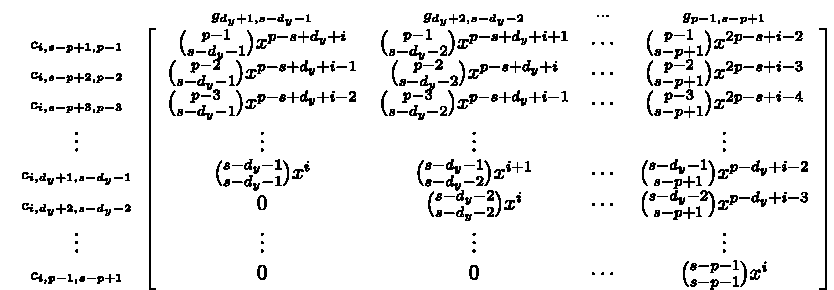
\includegraphics[width=\linewidth,height=0.78\textheight,keepaspectratio]{ccc2025-27-svg-01.pdf}\par




The rows correspond to the coefficients $c_{i,s-k,k}$ for $k=p-1,\dots,s-p+1$ as labeled on the left. Each row actually corresponds to $d_{x}+1$ coefficients, for $i\in[0,d_{x}]$, but for sake of space we condense these into a single row.\par




The columns correspond to $g_{d^{\prime},s-d^{\prime}}(x)$ for $d^{\prime}\in[d_{y}+1,p-1]$. Because $d^{\prime}>d_{y}$, these $g_{d^{\prime},s-d^{\prime}}(x)$ all should be $0$. The way to read off the value of $g_{d^{\prime},s-d^{\prime}}(x)$ is by looking at the corresponding column, and summing the product of each entry with the corresponding row coefficient $c_{i,s-k^{\prime},k^{\prime}}$, remembering that each row actually corresponds to $d_{x}+1$ rows for $i\in[0,d_{x}]$. The entries of the matrix were chosen according to the expansion of $g_{d^{\prime},s-d^{\prime}}(x)$ given in Claim 35.\par




Now, to prove that $c_{i,s-k,k}=0$ for all $i\in[0,d_{x}]$ and $k\in[0,p-1]$, we will backwards induct on the value of $i+k$, which we will denote by $t$. So assume that for $i^{\prime}+k^{\prime}>t$ that $c_{i^{\prime},s-k^{\prime},k^{\prime}}=0$. This is true for $t=d_{x}+(p-1)$, since there do not exist coefficients with larger values of $i^{\prime}+k^{\prime}$ (as $i^{\prime}\leq d_{x}$ and $k^{\prime}\leq p-1$).\par




Consider all the coefficients with $i+k=t$, meaning coefficients $c_{i,s-t+i,t-i}$ where $i\in[0,d_{x}]$ and $t-i,s-t+i\in[0,p-1]$. These coefficients correspond to $\leq d_{x}+1$ consecutive rows of the matrix with increasing values of $i$. Note that in each column, these coefficients only contribute to a single monomial $x^{i^{\prime}}$: namely, in the column for $g_{d^{\prime},s-d^{\prime}}$, the exponents of $x$ that appear for $i+k=t$ are all equal to $i^{\prime}=i+(k-(s-d^{\prime}))=t-s+d^{\prime}$. Thus, for any $g_{d^{\prime},s-d^{\prime}}(x)$ which has degree $<p$, we obtain a linear constraint on $c_{i,s-t+i,t-i}$ by restricting the corresponding column corresponding to the rows corresponding to the coefficients (we may also drop the powers of $x$, so that the coefficients of the linear constraint are simply binomial coefficients). For instance, for $t=p$, the column $g_{d^{\prime},s-d^{\prime}}$ gives us the constraint\par


\[\begin{gathered}
\begin{pmatrix}c_{1,s-p+1,p-1}&c_{2,s-p+2,p-2}&\cdots&c_{d_{x},s-p+d_{x},p-d_{x}}\end{pmatrix}\begin{pmatrix}\binom{p-1}{s-d^{\prime}}\\
\binom{p-2}{s-d^{\prime}}\\
\vdots\\
\binom{p-d_{x}}{s-d^{\prime}}\end{pmatrix}=0.
\end{gathered}\]




Our strategy may therefore be summarized as follows: for each $t\leq p-1+d_{x}$, assuming that there are $m$ coefficients of the form $c_{i,s-t+i,t-i}$, we will find $m$ consecutive columns such that the degree of $x$ in $g_{d^{\prime},s-d^{\prime}}(x)$ is $<p$. These columns will also satisfy that if we restrict the matrix to these columns and to the rows corresponding to the coefficients, the resulting $m\times m$ matrix has diagonal that lies above the lower left triangle of $0$’s. Then, by Lemma 33, we know these $m$ linear constraints are independent, telling us that $c_{i,s-t+i,t-i}=0$ for each $i$.\par




The columns will be chosen as follows.\par


\begin{itemize}


\item[] 
$\blacksquare$ 


For $t\geq p-1$, we are considering the $m=p-t+d_{x}$ coefficients\par


\[\begin{gathered}
c_{t-p+1,s-p+1,p-1},\nobreak\ c_{t-p+2,s-p+2,p-2},\nobreak\ \dots,\nobreak\ c_{d_{x},s-t+d_{x},t-d_{x}}.
\end{gathered}\]


We pick the first $p-t+d_{x}$ columns of the matrix, corresponding to $g_{d_{y}+1,s-d_{y}-1},$ $g_{d_{y}+2,s-d_{y}-2},$ $\dots,$ $g_{p+d_{x}+d_{y}-t,s+t-p-d_{x}-d_{y}}$. Each of $g_{d^{\prime},s-d^{\prime}}(x)$ for $d^{\prime}\in[d_{y}+1,p+d_{x}+d_{y}-t]$ is a polynomial in $x$. Using the inductive hypothesis that $c_{i^{\prime},s-k^{\prime},k^{\prime}}=0$ for $i^{\prime}+k^{\prime}>t$, we see that the maximum degree of $x$ in any of these polynomials is $\leq i+k-\min(s-d^{\prime})=t-(s+t-p-d_{x}-d_{y})=p+d_{x}+d_{y}-s<d_{x}+d_{y}<p$.\par





\item[] 
$\blacksquare$ 


For $s-d_{y}-1\leq t<p-1$, we are looking at the $d_{x}+1$ coefficients\par


\[\begin{gathered}
c_{0,s-t,t},c_{1,s-t+1,t-1},\dots,c_{d_{x},s-t+d_{x},t-d_{x}}.
\end{gathered}\]


Consider the $d_{x}+1$ columns corresponding to $g_{d_{y}+1,s-d_{y}-1},\nobreak\ \dots,\nobreak\ g_{d_{x}+d_{y}+1,s-d_{x}-d_{y}-1}$. Because $t\geq s-d_{y}-1$, the submatrix has nonzero diagonal. The largest exponent of $x$ in any of these columns is $\leq i+k-(s-d_{x}-d_{y}-1)\leq t-s+d_{x}+d_{y}-1<d_{x}+d_{y}-1<p$.\par





\item[] 
$\blacksquare$ 


For $t<s-d_{y}-1$, let $\hat{d}=\min(d_{x},p-1-s+t)$. We consider the $\hat{d}+1$ coefficients\par


\[\begin{gathered}
c_{0,s-t,t},\nobreak\ c_{1,s-t+1,t-1},\nobreak\ \dots,\nobreak\ c_{\hat{d},p-1,t-\hat{d}}.
\end{gathered}\]


Look at the $\hat{d}+1$ columns corresponding to $g_{s-t,t},\nobreak\ \dots,\nobreak\ g_{s-t+\hat{d},t-\hat{d}}$. This matrix has nonzero diagonal. The largest degree of $x$ in any of these columns is $\leq i+k-(t-\hat{d})\leq\hat{d}<p$.\par





\end{itemize}





\par\medskip\noindent\textbf{Case 3: $d_{x}+d_{y}<s\leq p-1$.}\par




Similar to the previous case, we consider the following matrix, interpreted the same way as before.\par




\par\noindent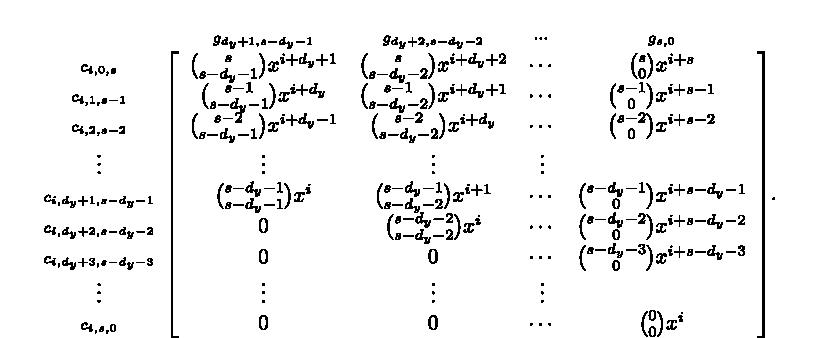
\includegraphics[width=\linewidth,height=0.78\textheight,keepaspectratio]{ccc2025-27-svg-03.pdf}\par




As in the previous case, we will downwards induct on the value of $i+k=t$. Assume that for $i^{\prime}+k^{\prime}>t$ it holds that $c_{i^{\prime},s-k^{\prime},k^{\prime}}=0$. This is true for $t=d_{x}+s$ (the maximal possible value of $i+k$) since there do not exist coefficients with larger values of $i^{\prime}+k^{\prime}$.\par




We again consider all $m$ coefficients satisfying $i+k=t$. These occupy a number of consecutive rows of the matrix. Furthermore, for any column with degree in $x$ less than $p$, restricting that column to those rows gives a linear constraint on the coefficients. Thus, we again demonstrate, for each $t$, $m$ consecutive columns that each have exponent in $x$ less than $p$. Restricting these columns to the coefficient rows will result in a $m\times m$ submatrix lying above the lower left triangle of $0$’s, which is full rank by Lemma 33, implying that all $m$ coefficients must in fact be $0$.\par




\begin{itemize}


\item[] 
$\blacksquare$ 


For $t\geq s$, we are interested in the $s-t+d_{x}+1$ coefficients\par


\[\begin{gathered}
c_{t-s,0,s},\nobreak\ c_{t-s+1,1,s-1},\nobreak\ \dots,\nobreak\ c_{d_{x},s-t+d_{x},t-d_{x}}.
\end{gathered}\]


Look at the first $s-t+d_{x}+1$ columns, which correspond to $g_{d^{\prime},s-d^{\prime}}$ for $d^{\prime}\in[d_{y}+1,s-t+d_{x}+d_{y}+1]$. The maximum degree of any of these polynomials is $i+k-(t-d_{x}-d_{y}-1)=d_{x}+d_{y}+1<p$.\par





\item[] 
$\blacksquare$ 


For $s-d_{y}-1\leq t<s$, we consider the $d_{x}+1$ coefficients\par


\[\begin{gathered}
c_{0,s-t,t},\nobreak\ c_{1,s-t+1,t-1},\nobreak\ \dots,\nobreak\ c_{d_{x},s-t+d_{x},t-d_{x}}.
\end{gathered}\]


The columns we are interested in are $g_{d_{y}+1,s-d_{y}-1},\nobreak\ \dots,\nobreak\ g_{d_{x}+d_{y}+1,s-d_{x}-d_{y}-1}$. Since $t\geq s-d_{y}-1$, the submatrix has nonzero diagonal. The maximum degree of any of these polynomials is $\leq i+k-(s-d_{x}-d_{y}-1)=t-s+d_{x}+d_{y}+1<d_{x}+d_{y}+1<p$.\par





\item[] 
$\blacksquare$ 


For $t<s-d_{y}-1$, let $\hat{d}=\min(d_{x},t)$. Then we are considering the following $\hat{d}+1$ coefficients.\par


\[\begin{gathered}
c_{0,s-t,t},\nobreak\ c_{1,s-t+1,t-1},\nobreak\ \dots,\nobreak\ c_{\hat{d},s-t+\hat{d},t-\hat{d}}.
\end{gathered}\]


For these, we will look at the $\hat{d}+1$ columns corresponding to $g_{s-t,t},\nobreak\ \dots,\nobreak\ g_{s-t+\hat{d},t-\hat{d}}$. This clearly has nonzero diagonal, and the maximum degree of $x$ in any of these polynomials is $i+k-(t-\hat{d})=\hat{d}<p$.\par





\end{itemize}


$\blacktriangleleft$\par



% SOURCE-ID Thmtheorem36


\par\medskip\noindent\textbf{
\textbf{Theorem 36}\textbf{.}
}\par



\emph{For $p\geq d_{x}+d_{y}+2$, the dimension of the local code is $\frac{1}{2}\cdot(d_{x}+1)(d_{y}+1)(d_{x}+d_{y}+2)$.}\par



% END-SOURCE-ID Thmtheorem36




\par\medskip\noindent\textbf{Proof.}\par




From Lemma 34, we know that $c_{ijk}=0$ for all $i\in[0,d_{x}]$ and $j+k>d_{x}+d_{y}$. Thus we can write\par


\[\begin{gathered}
\displaystyle f(x,y,z) \displaystyle=\sum_{\begin{subarray}{c}0\leq i\leq d_{x}\\
0\leq j+k\leq d_{x}+d_{y}\end{subarray}}c_{ijk}x^{i}y^{j}z^{k}.
\end{gathered}\]


Note that $c_{i^{\prime}j^{\prime}k^{\prime}}x^{i^{\prime}}y^{j^{\prime}}(xy+z)^{k^{\prime}}=\sum_{0\leq k\leq k^{\prime}}\binom{k^{\prime}}{k}x^{k^{\prime}-k+i^{\prime}}y^{k^{\prime}-k+j^{\prime}}z^{k}$ and in particular the sum of the exponents of $y$ and $z$ is always $j^{\prime}+k^{\prime}$, so in particular the value of $g_{jk}(x)$ only depends on coefficients $c_{i^{\prime}j^{\prime}k^{\prime}}$ were $j^{\prime}+k^{\prime}=j+k$ (note also that we’re now in the setting where $j+k\leq d_{x}+d_{y}<p$, so $g(x,y,z)=f(x,y,xy+z)$ without having to reduce modulo $y^{p}-y$).\par




Again, we will use the fact that for all $j>d_{y}$ and $k\in[0,p-1]$, it holds that $g_{jk}(x)=0\nobreak\ \forall x\in\mathbb{F}_{p}$. Note that $g_{jk}(x)$ could have degree as large as $2d_{x}+d_{y}$ which could be larger than $p$. We thus let $\hat{g}_{jk}(x)$ denote $g_{jk}(x)$ reduced modulo $x^{p}-x$. The condition that $g_{jk}(x)=0\nobreak\ \forall x\in\mathbb{F}_{p}$ then is equivalent to $\hat{g}_{jk}(x)\equiv 0$.\par




We will work through the polynomials $\hat{g}_{jk}(x)$ and set each to $0$ by choosing coefficients $c_{ijk}$ appropriately. We will consider all the polynomials $\hat{g}_{jk}$ with a fixed value of $j+k$, denoted by $s$, simultaneously.\par




As such, let $d_{y}<s\leq d_{x}+d_{y}$. The relevant polynomials $g_{jk}(x)$ that evaluate to $0$ everywhere are $g_{d_{y}+1,s-d_{y}-1},\dots,g_{s,0}$, and the relevant coefficients are $c_{i,0,s},\dots,c_{i,s,0}$, where $i\in[0,d_{x}]$. The dependency of $g_{d^{\prime},s-d^{\prime}}$ on the coefficients is given in the following matrix, interpretted the same as before.\par




\par\noindent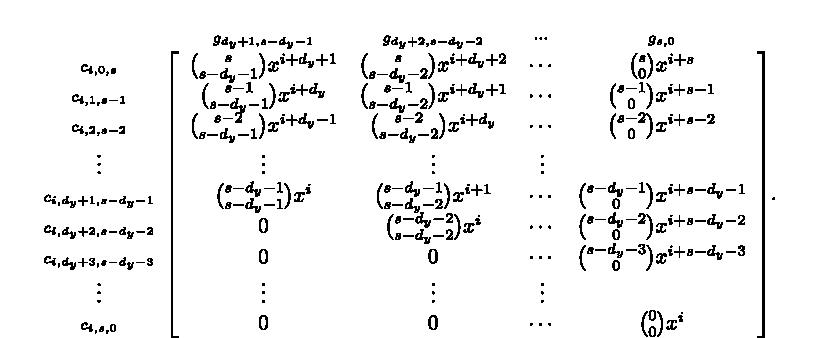
\includegraphics[width=\linewidth,height=0.78\textheight,keepaspectratio]{ccc2025-27-svg-03.pdf}\par




We will set the coefficients $c_{i,s-k,k}$ starting with those with the largest value of $t:=i+k$, which is $d_{x}+s$, and proceeding downwards. We will show that if we’ve already set all coefficients $c_{i,s-k,k}$ with $i+k>t$, then the degree of $\hat{g}_{d^{\prime},s-d^{\prime}}(x)$ is $\leq d^{\prime}+t-s$ (that is, all larger monomials have been set to $0$ by the previous choices of coefficient assignments). This is certainly satisfied in the base case: if $t=d_{x}+s$, then since $i\leq d_{x}$ we have that the largest power of $x$ in any $g_{d^{\prime},s-d^{\prime}}(x)$ is $d_{x}+d^{\prime}=d^{\prime}+t-s$. This largest exponent can only decrease when we pass to $\hat{g}_{d^{\prime},s-d^{\prime}}(x)$.\par




Now, suppose that we’re part way through this process and have already set the values for all $c_{i,s-k,k}$ where $i+k>t$. The number of ways we have to set the values $c_{t-k,s-k,k}$ is as follows.\par




\begin{itemize}


\item[] 
$\blacksquare$ 


For $t=d_{x}+s,$ $d_{x}+s-1,$ $\dots,$ $d_{x}+d_{y}+1$, the coefficients of interest are $c_{t-s,0,s},$ $c_{t-s+1,1,s-1},$ $\dots,$ $c_{d_{x},s+d_{x}-t,t-d_{x}}$. We will show that these must all be set to $0$. We look at the columns corresponding to $g_{d_{y}+1,s-d_{y}-1},\nobreak\ \dots,\nobreak\ g_{d_{x}+d_{y}-t+s+1,t-d_{x}-d_{y}-1}$. Note that there are as many columns as coefficients. By the inductive assumption, the maximal degree of column $g_{d^{\prime},s-d^{\prime}}$ is $\leq d^{\prime}+t-s\leq d_{x}+d_{y}+1<p$. Thus the coefficient of $x^{d^{\prime}+t-s}$ in $g_{d^{\prime},s-d^{\prime}}(x)$, which is equal to $\sum_{t-d_{x}\leq k\leq s}\binom{k}{s-d^{\prime}}c_{t-k,s-k,k}$, must also be $0$. This gives us the following linear system of equations:\par


\[\begin{gathered}
\begin{pmatrix}c_{t-s,0,s}\\
c_{t-s+1,1,s-1}\\
\vdots\\
c_{d_{x},s-t+d_{x},t-d_{x}}\end{pmatrix}^{T}\cdot\begin{pmatrix}\binom{s}{s-d_{y}-1}&\binom{s}{s-d_{y}-2}&\cdots&\binom{s}{t-d_{x}-d_{y}-1}\\
\binom{s-1}{s-d_{y}-1}&\binom{s-1}{s-d_{y}-2}&\cdots&\binom{s-1}{t-d_{x}-d_{y}-1}\\
\vdots&\vdots&&\vdots\\
\binom{t-d_{x}}{s-d_{y}-1}&\binom{t-d_{x}}{s-d_{y}-2}&\cdots&\binom{t-d_{x}}{t-d_{x}-d_{y}-1}\end{pmatrix}=0,
\end{gathered}\]


where the matrix is also a top left submatrix of the aforementioned matrix, ignoring the powers of $x$. Since $s>s-d_{y}-1$, this matrix has nonzero diagonal and by Lemma 33 is invertible. This implies that $c_{t-k,s-k,k}=0$ for all $t-d_{x}\leq k\leq s$.\par




Now, we’ve set all $c_{ijk}$ with $j+k\geq t$. It remains to show that $\hat{g}_{d^{\prime},s-d^{\prime}}(x)$ is now degree $\leq d^{\prime}+t-s-1$. We already have that $\hat{g}_{d^{\prime},s-d^{\prime}}(x)$ was degree $\leq d^{\prime}+t-s$ from the inductive assumption. For any $\hat{g}_{d^{\prime},s-d^{\prime}}(x)$, the coefficient of the $x^{d^{\prime}+t-s}$ term is the sum of the coefficients of $x^{d^{\prime}+t-s}$ and $x^{d^{\prime}+t-s+(p-1)}$ in $g_{d^{\prime},s-d^{\prime}}(x)$. But recall that we’ve set all $c_{ijk}$ with $j+k\geq t$ to $0$, so both these coefficients in $g_{d^{\prime},s-d^{\prime}}$ must be $0$. Therefore, $\hat{g}_{d^{\prime},s-d^{\prime}}(x)$ is degree $\leq d^{\prime}+t-s-1$.\par





\item[] 
$\blacksquare$ 


Next, for $t=d_{x}+d_{y},\dots,s+1$, we are looking at the $s+d_{x}-t+1>s-d_{y}$ coefficients $c_{t-s,0,s},\dots,c_{d_{x},s-t+d_{x},t-d_{x}}$. We have so far that all $\hat{g}_{d^{\prime},s-d^{\prime}}(x)$ have degree $\leq d^{\prime}+t-s$. The coefficient of $x^{d^{\prime}+t-s}$ in $\hat{g}_{d^{\prime},s-d^{\prime}}(x)$ is equal to the sum of the coefficients of $x^{d^{\prime}+t-s}$ and $x^{d^{\prime}+t-s+(p-1)}$ in $g_{d^{\prime},s-d^{\prime}}(x)$, which in turn is equal to\par


\[\begin{gathered}
\sum_{t-d_{x}\leq k\leq s}\binom{k}{s-d^{\prime}}\cdot c_{t-k,s-k,k}+\sum_{0\leq k\leq s}\binom{k}{s-d^{\prime}}\cdot c_{t-k+(p-1),s-k,k},
\end{gathered}\]


where in the second summation the terms $c_{t-k+(p-1),s-k,k}$ that don’t exist are understood to be $0$. Note that we’ve already set the values of $c_{t-k+(p-1),s-k,k}$. Thus, in order to set ($\blacksquare$ \ensuremath{\blacktriangleright} 4.2) to $0$, we need to choose $c_{t-k,s-k,k}$, $t-d_{x}\leq k\leq s$ so that\par


\[\begin{gathered}
\sum_{t-d_{x}\leq k\leq s}\binom{k}{s-d^{\prime}}\cdot c_{t-k,s-k,k}=-\sum_{0\leq k\leq s}\binom{k}{s-d^{\prime}}\cdot c_{t-k+(p-1),s-k,k}.
\end{gathered}\]


There are $s-d_{y}$ such equations for the $s-d_{y}$ polynomials $\hat{g}_{d^{\prime},s-d^{\prime}}(x)$, which are all independent by Lemma 33 since $s\geq s-d_{y}-1$. Then, there are $p^{s+d_{x}-t+1-(s-d_{y})}=p^{d_{x}+d_{y}+1-t}$ ways to choose the coefficients $c_{t-k,s-k,k}$. We remark also that once $c_{t-s,0,s},$ $\dots,$ $c_{d_{x},s-t+d_{x},t-d_{x}}$ are set, all $\hat{g}_{d^{\prime},s-d^{\prime}}(x)$ must have degree $\leq d^{\prime}+t-s-1$ since we chose the values so that the coefficient of $x^{d^{\prime}+t-s}$ was $0$ for all columns.\par





\item[] 
$\blacksquare$ 


The next case is $t=s,\nobreak\ s-1,\nobreak\ \dots,\nobreak\ d_{x}$. In this case, we are looking at the $d_{x}+1$ coefficients $c_{0,s-t,t},\dots,c_{d_{x},s-t+d_{x},t-d_{x}}$. We have so far that all $\hat{g}_{d^{\prime},s-d^{\prime}}(x)$ have degree $\leq d^{\prime}+t-s$, and the coefficient of $x^{d^{\prime}+t-s}$ in $\hat{g}_{d^{\prime},s-d^{\prime}}(x)$ is equal to the sum of the coefficients of $x^{d^{\prime}+t-s}$ and $x^{d^{\prime}+t-s+(p-1)}$ in $g_{d^{\prime},s-d^{\prime}}(x)$. Similar to the previous case, this results in $s-d_{y}$ independent linear equations (by Lemma 33, using the fact that $t\geq s-d_{y}-1$. Thus, there are $p^{d_{x}+d_{y}+1-s}$ ways to set $c_{0,s-t,t},\dots,c_{d_{x},s-t+d_{x},t-d_{x}}$. Note that after we’ve set these coefficients, the degree of $\hat{g}_{d^{\prime},s-d^{\prime}}(x)$ necessarily must be $\leq d^{\prime}+t-s-1$ by choice of these coefficients.\par





\item[] 
$\blacksquare$ 


If $t=d_{x}-1,\dots,s-d_{y}$, then the coefficients we care about are $c_{0,s-t,t},\dots,c_{t,s,0}$. We have that $\hat{g}_{d^{\prime},s-d^{\prime}}(x)$ has degree $\leq d^{\prime}+t-s$ and wish to set the $c_{t-k,s-k,k}$ so that the coefficient of $x^{d^{\prime}+t-s}$ is $0$. As before, this results in $s-d_{y}$ linearly independent equations, which are independent because $t\geq s-d_{y}-1$. Thus, there are $p^{t+1-s+d_{y}}$ ways to set the coefficients $c_{t-k,s-k,k}$. The degrees of all $s-d_{y}$ polynomials $\hat{g}_{t-k,s-k,k}(x)$ are now $\leq d^{\prime}+t-s-1$.\par





\item[] 
$\blacksquare$ 


For $t=s-d_{y}-1,\dots,0$, we are considering the $t+1$ coefficients $c_{0,s-t,t},\dots,c_{t,s,0}$. Note also that for $d^{\prime}<s-t$, we must already have that $\hat{g}_{d^{\prime},s-d^{\prime}}(x)\equiv 0$ since the maximum degree, if it exists, is already $\leq d^{\prime}+t-s$. So, we look at the $t+1$ polynomials $\hat{g}_{s-t,t}(x),\dots,\hat{g}_{s,0}(x)$. Since we want to set the coefficient of $x^{d^{\prime}+t-s}$ to be $0$, this results in $t+1$ linearly independent equations in $c_{0,s-t,t},\dots,c_{t,s,0}$. So there is exactly one way to set $c_{0,s-t,t},\dots,c_{t,s,0}$ to make all these coefficients $0$.\par





\end{itemize}




In total, for $d_{y}<s\leq d_{x}+d_{y}$, if $C_{s}$ is the number of ways to assign all the coefficients $c_{i,s-k,k}$, then\par


\[\begin{gathered}
\displaystyle\log_{p}C_{s} \displaystyle=0+\sum_{t=s+1}^{d_{x}+d_{y}}(d_{x}+d_{y}+1-t)+\sum_{t=d_{x}}^{s}(d_{x}+d_{y}+1-s) \\
\displaystyle\nobreak\ \nobreak\ \nobreak\ \nobreak\ +\sum_{t=s-d_{y}}^{d_{x}-1}(t+1-s+d_{y})+0 \\
\displaystyle=(d_{y}+1)(d_{x}+d_{y}+1-s).
\end{gathered}\]


Furthermore, if $j+k=s\leq d_{y}$, then $f(x,y,xy+z)$ is always degree $\leq d_{y}$ in $y$, so all such coefficients $c_{ijk}$ are permissible. There are $(d_{x}+1)\cdot\binom{d_{y}+2}{2}$ such coefficients. In total, this gives that the dimension of the local code is\par


\[\begin{gathered}
\displaystyle(d_{x}+1)\cdot\binom{d_{y}+2}{2}+\sum_{s=d_{y}+1}^{d_{x}+d_{y}}\left((d_{y}+1)(d_{x}+d_{y}+1-s)\right) \\
\displaystyle=\frac{1}{2}\cdot(d_{x}+1)(d_{y}+1)(d_{x}+d_{y}+2).
\end{gathered}\]


$\blacktriangleleft$\par







\par\medskip\noindent\textbf{
5 Code Testability}\par




In this section, we will work with the field size $q=p$ being a prime. The main reason is that we will need results from Section 4.2 about the degree of codewords in $C_{d_{x},d_{y}}$, viewed as low degree polynomials.\par




\par\medskip\noindent\textbf{
5.1 Testability of the Local Code at a Vertex}\par




In this section we prove that $C_{v}\cong C_{d_{x},d_{y}}$ (as defined in Lemma 30) is agreement-testable whenever $d_{x},d_{y}<p/4$. Our definition of agreement testability (see Definition 15) applies to HDX codes. Let us restate it in a form that is specialized for $C_{v}$:\par



% SOURCE-ID Thmtheorem37


\par\medskip\noindent\textbf{
\textbf{Definition 37}\textbf{.}
}\par



\emph{The local code $C_{v}$ defined in (15) is $(\epsilon,\rho(\cdot))$-agreement testable if whenever we are given a collection of $z_{e}\in C_{e}$ for each $e\ni v$, such that}\par


\[\begin{gathered}
\alpha:=\operatorname*{\mathbb{P}}_{uw\in X_{v}(1)}[z_{uv}(T_{uvw})\neq z_{wv}(T_{uvw})]<\epsilon
\end{gathered}\]


\emph{then there exists some $x\in C_{v}$ such that}\par


\[\begin{gathered}
\operatorname*{\mathbb{P}}_{u\in X(0)}(z_{uv}\neq x|_{T_{uv}})\leq\rho(\alpha).
\end{gathered}\]



% END-SOURCE-ID Thmtheorem37



Recall $C_{v}\cong C_{d_{x},d_{y}}$. The local views have two kinds. Let us see the case where $v=K_{1}$: Cosets of $H_{2}$ correspond to lines $(x,b,c)$ for all $b,c\in\mathbb{F}_{p}$. Cosets of $H_{3}$ correspond to lines $(a,y,ay+c)$ for all $a,c\in\mathbb{F}$.
Therefore, the local views can be packaged through $X,Y$, which will be collections of degree $d_{2}$ and $d_{3}$ polynomials on the lines corresponding to cosets of $H_{2}$ and $H_{3}$, respectively.\par




The following theorem will immediately imply local testability.\par



% SOURCE-ID Thmtheorem38


\par\medskip\noindent\textbf{
\textbf{Theorem 38}\textbf{.}
}\par



\emph{Let $X,Y:\mathbb{F}_{p}^{3}\to\mathbb{F}_{p}$ be such that}\par


\begin{itemize}


\item[] 
$\blacksquare$ 


\emph{For each }$b,c$\emph{, the }$x$\emph{ degree of }$X(x,b,c)$\emph{ is at most }$d_{x}$\emph{.}\par





\item[] 
$\blacksquare$ 


\emph{For each }$a,c$\emph{, the }$y$\emph{ degree of }$Y(a,y,ay+c)$\emph{ is at most }$d_{y}$\emph{.}\par





\end{itemize}


\emph{Then if $\mathbb{P}[X(x,y,z)\not=Y(x,y,z)]=\delta^{3}$ so that $p\geq d_{x}+d_{y}+2\max(d_{x},d_{y})+4\delta p$, there exists codeword $Q(x,y,z)\in C_{d_{x},d_{y}}$ such that}\par


\[\begin{gathered}
\mathbb{P}_{b,c}[X(x,b,c)\not=Q(x,b,c)]+\mathbb{P}_{a,c}[Y(a,y,ay+c)\not=Q(a,y,ay+c)]\leq 4\delta.
\end{gathered}\]



% END-SOURCE-ID Thmtheorem38



Before proving Theorem 38, let us see that it immediately implies agreement testability.\par



% SOURCE-ID Thmtheorem39


\par\medskip\noindent\textbf{
\textbf{Corollary 39}\textbf{.}
}\par



\emph{If $d_{x},d_{y}<\frac{p}{4}$, the local code $C_{v}=C_{d_{x},d_{y}}$ is $\left(\left(\frac{p/2-(d_{x}+d_{y})}{4p}\right)^{3},4(\cdot)^{1/3}\right)$-agreement testable.}\par



% END-SOURCE-ID Thmtheorem39



\par\medskip\noindent\textbf{Proof.}\par




Without loss of generality, let $v$ be the coset $K_{1}$ in $X(G;K_{1},K_{2},K_{3})$ (the argument applies to other choices of $v$ since $G$ acts transitively on the code $C_{v}$, see Claim 26).
Then every edge $e\ni v$ is of type $2$ or type $3$. Recall from Theorem 1 that type 2 edges $e$ are cosets $\{gh_{2}(x)\}_{x}$ while type 3 edges $e$ correpsond to cosets of the form $\{gh_{3}(y)\}_{y}$.
Given a collection of local views $z_{e}\in C_{e}$, we define functions $X,Y:\mathbb{F}_{p}^{3}\to\mathbb{F}_{p}$ in the following way:\par


\[\begin{gathered}
\displaystyle X(x,b,c)=z_{gh_{2}}(gh_{2}(x))\nobreak\ \text{where }g=\iota^{-1}(0,b,c), \\
\displaystyle Y(a,y,ay+c)=z_{gh_{3}}(gh_{3}(y))\nobreak\ \text{where }g=\iota^{-1}(a,0,c).
\end{gathered}\]


Here $\iota$ is the embedding of elements in $K_{1}$ to $\mathbb{F}_{p}^{3}$ as used in the proof of Lemma 30. Since $z_{gh_{2}}(gh_{2}(x))$ has degree at most $d_{2}$ and $z_{gh_{3}}(gh_{3}(y))$ has degree at most $d_{3}$, $X$ and $Y$ satisfy the conditions in the theorem statement for $d_{x}=d_{2},d_{y}=d_{3}$. Also by construction of $X$ and $Y$\par


\[\begin{gathered}
\displaystyle\operatorname*{\mathbb{P}}_{uw\in X_{v}(1)}[z_{uv}(T_{uvw})\neq z_{wv}(T_{uvw})]=\mathbb{P}_{x,y,z}[X(x,y,z)\not=Y(x,y,z)]
\end{gathered}\]




Similarly, given a codeword $Q\in C_{d_{x}.d_{y}}$, by Lemma 30 we can define its corresponding codeword $f\in C_{v}$ as\par


\[\begin{gathered}
f(g)=Q(\iota(g)).
\end{gathered}\]


Then the disagreement probability between $z_{e}$ and $f$ satisfies:\par


\[\begin{gathered}
2\operatorname*{\mathbb{P}}_{u\in X(0)}(z_{uv}\neq f|_{T_{uv}})=\mathbb{P}_{b,c}[X(x,b,c)\not=Q(x,b,c)]+\mathbb{P}_{a,c}[Y(a,y,ay+c)\not=Q(a,y,ay+c)].
\end{gathered}\]




Now applying Theorem 38 to $z_{e}$ and $f$ we have that the local code $C_{v}$ is


$\left(\left(\frac{p-(d_{x}+d_{y})-2\max(d_{x},d_{y})}{4p}\right)^{3}\geq\left(\frac{p/2-(d_{x}+d_{y})}{4p}\right)^{3},4(\cdot)^{1/3}\right)$-agreement testable.
$\blacktriangleleft$\par




We now move to prove Theorem 38.
Let $S$ denote the set of all points $(x,y,z)$ on which $X(x,y,z)\not=Y(x,y,z)$. Consider all polynomials $e(x,y,z)$ that are degree $\delta p$ in $x$, and degree $\delta p$ in $y$ in $e(x,y,xy+z)$. By Theorem 36 , the dimension of the space of such polynomials is $(\delta p+1)^{3}$. Thus, by dimension counting, there is a nonzero polynomial $E(x,y,z)$ that evaluates to $0$ on all points of $S$. Then, we have that for all $x,y,z$, $X(x,y,z)E(x,y,z)=Y(x,y,z)E(x,y,z)$.\par




We have that $X(x,y,z)E(x,y,z)$ is degree $d_{x}+\delta p$ in $x$, and $Y(x,y,xy+z)E(x,y,xy+z)$ is degree $d_{y}+\delta p$ in $y$. Thus there is a polynomial $P(x,y,z)$ that is degree $d_{x}+\delta p$ in $x$, and degree $d_{y}+\delta p$ in $y$ in $P(x,y,xy+z)$, that agrees on all points. (To see this, we can write $P(x,y,z)$ as a polynomial that is degree $q-1$ in each of $x,y,z$. Since $P(x,y_{0},z_{0})$ has the same evaluation as a degree $d_{x}+\delta p$ polynomial for each $y_{0},z_{0}$, it follows that $P$ must be degree $d_{x}+\delta p$ in $x$. Next, by Lemma 34, we have that $P$ must be combined degree $d_{x}+\delta p+d_{y}+\delta p<q$ in $y$ and $z$. Thus, $P(x,y,xy+z)$ is degree $<q$ in $y$. Since $P(x_{0},y,x_{0}y+z_{0})$ has the same evaluation as a degree $d_{y}+\delta p$ polynomial for each $x_{0},z_{0}$, it follows that $P(x,y,xy+z)$ must actually be degree $d_{y}+\delta p$ in $y$.)\par




We may write\par


\[\begin{gathered}
X(x,y,z)E(x,y,z)=Y(x,y,z)E(x,y,z)=P(x,y,z)\nobreak\ \forall x,y,z.
\end{gathered}\]


We’d like to formally divide $P(x,y,z)$ by $E(x,y,z)$ to obtain a polynomial $Q(x,y,z)$ that is degree $d_{x}$ in $x$ and degree $d_{y}$ in the skew-$y$ direction.\par



% SOURCE-ID Thmtheorem40


\par\medskip\noindent\textbf{
\textbf{Lemma 40}\textbf{.}
}\par



\emph{There exists a polynomial $Q(x,y,z)$ that is degree $d_{x}$ in $x$ and degree $d_{y}$ in the skew-$y$ direction, such that $E(x,y,z)Q(x,y,z)=P(x,y,z).$}\par



% END-SOURCE-ID Thmtheorem40




\par\medskip\noindent\textbf{Proof.}\par




First, suppose $P(x,y,z)$ and $E(x,y,z)$ share a common factor $F(x,y,z)\not\equiv E(x,y,z)$ of degree $(e,f)$ in the $x$ and skew-$y$ directions, and set\par


\[\begin{gathered}
P(x,y,z)\equiv\bar{P}(x,y,z)F(x,y,z)\nobreak\ \text{and}\nobreak\ E(x,y,z)\equiv\bar{E}(x,y,z)F(x,y,z)
\end{gathered}\]


so that $\bar{P}(x,y,z)$ and $\bar{E}(x,y,z)$ share no common factors.\par




Note that whenever $F(x,y_{0},z_{0})$ is not the $0$ polynomial (in $x$), then we have that $\bar{E}(x,y_{0},z_{0})|\bar{P}(x,y_{0},z_{0})$. Since the combined degree of $y$ and $z$ in $F(x,y,z)$ is $\leq e+f<|\mathbb{F}|$ by Lemma 34 and $F(x,y,xy+z)$ is degree $f$ in $y$, there can be at most $f$ values of $y_{0}\in\mathbb{F}$ for which $F(x,y_{0},z)\equiv 0$ and also at most $f$ values of $z_{0}\in\mathbb{F}$ for which $F(x,y,z_{0})\equiv 0$. Let $Y_{x}$ denote the values of $y_{0}$ for which $F(x,y_{0},z)\not\equiv 0$ and $Z_{x}$ denote the values $z_{0}$ for which $F(x,y,z_{0})\not\equiv 0$, so that $|Y_{x}|,|Z_{x}|\geq|\mathbb{F}|-f$. For any $y_{0}\in Y_{x}$, there can be at most $e+f$ values of $z_{0}$ for which $f(x,y_{0},z_{0})\equiv 0$, and for any $z_{0}\in Z_{x}$, there can be at most $e+f$ values of $y_{0}$ for which $f(x,y_{0},z_{0})\equiv 0$. Thus, there are at least $\max(|Y_{x}|,|Z_{x}|)(|\mathbb{F}|-e-f)$ pairs $(y_{0},z_{0})\in\mathbb{F}\times\mathbb{F}$ for which $\bar{E}(x,y_{0},z_{0})|\bar{P}(x,y_{0},z_{0})$. Let the set of such pairs $(y_{0},z_{0})$ be denoted by $M_{x}$. We may show a similar statement for the skew-$y$ direction, that there is a set $M_{y}$ of size at least $\max(|Z_{x}|,|Z_{y}|)(|\mathbb{F}|-e-f)$ consisting of pairs $(x_{0},z_{0})$ for which $\bar{E}(x_{0},y,x_{0}y+z_{0})|\bar{P}(x_{0},y,x_{0}y+z_{0})$ as polynomials in $y$.\par




Our goal is to show that $\bar{E}(x,y,z)$ divides $\bar{P}(x,y,z)$. Assume for the sake of contradiction that $\bar{P}(x,y,z)$ and $\bar{E}(x,y,z)$ have no common factors. Let the degree of $\bar{E}(x,y,z)$ be $(a^{\prime}=a-e,b^{\prime}=b-f)$ in the $x$ and skew-$y$ directions, so that $\bar{P}(x,y,z)$ has degree $(d_{x}+a^{\prime},d_{y}+b^{\prime})$ in the $x$ and skew-$y$ directions.
Assume without loss of generality that $a^{\prime}\geq b^{\prime}$, otherwise we can consider the change of basis $P^{\prime}(x,y,z)=\bar{P}(y,x,xy-z)$ and $E^{\prime}(x,y,z)=\bar{E}(y,x,xy-z)$.\par




Write\par


\[\begin{gathered}
\displaystyle\bar{P}(x,y,z) \displaystyle\equiv P_{0}(y,z)+P_{1}(y,z)x+\cdots+P_{a^{\prime}+d_{x}}(y,z)x^{a^{\prime}+d_{x}} \\
\displaystyle\bar{E}(x,y,z) \displaystyle\equiv E_{0}(y,z)+E_{1}(y,z)x+\cdots+E_{a^{\prime}}(y,z)x^{a^{\prime}}.
\end{gathered}\]


Then, $\bar{P}(x,y,z)$ and $\bar{E}(x,y,z)$ have a common factor if there exists $A(x,y,z)$ that is degree $\leq a^{\prime}-1$ in $x$ and $B(x,y,z)$ that is degree $\leq a^{\prime}+d_{x}-1$ in $x$ such that\par


\[\begin{gathered}
\bar{P}(x,y,z)A(x,y,z)=\bar{E}(x,y,z)B(x,y,z),
\end{gathered}\]


or\par


\[\begin{gathered}
\displaystyle P_{a^{\prime}+d_{x}}A_{a^{\prime}-1} \displaystyle=E_{a^{\prime}}B_{a^{\prime}+d_{x}-1} \\
\displaystyle P_{a^{\prime}+d_{x}-1}A_{a^{\prime}-1}+P_{a^{\prime}+d_{x}}A_{a^{\prime}-2} \displaystyle=E_{a^{\prime}-1}B_{a^{\prime}+d_{x}-1}+E_{a^{\prime}}B_{a^{\prime}+d_{x}-2} \\
\displaystyle\vdots \\
\displaystyle P_{0}A_{0} \displaystyle=E_{0}B_{0}.
\end{gathered}\]


These equations are linear in $A_{i}$ and $-B_{i}$ and can be summarized by the following $(2a^{\prime}+d_{x})\times(2a^{\prime}+d_{x})$ matrix:\par




\[\begin{gathered}
M(\bar{P},\bar{E})(y,z)=\begin{pmatrix}P_{a^{\prime}+d_{x}}&P_{a^{\prime}+d_{x}-1}&\cdots&\cdots&\cdots&P_{0}&0&\cdots&0\\
0&P_{a^{\prime}+d_{x}}&&\cdots&\cdots&P_{1}&P_{0}&\cdots&0\\
\vdots&\ddots&\ddots&&&&\ddots&\ddots&\vdots\\
0&\cdots&0&P_{a^{\prime}+d_{x}}&\cdots&\cdots&\cdots&P_{1}&P_{0}\\
E_{a^{\prime}}&E_{a^{\prime}-1}&\cdots&E_{1}&E_{0}&0&\cdots&\cdots&0\\
\vdots&\ddots&&&&&\ddots&&\vdots\\
\vdots&&\ddots&&&&&\ddots&0\\
0&\cdots&\cdots&\cdots&0&E_{a^{\prime}}&E_{a^{\prime}-1}&\cdots&E_{0}\end{pmatrix}
\end{gathered}\]


consisting of $a^{\prime}$ rows with $\bar{P}$ entries and $a^{\prime}+d_{x}$ rows of $\bar{E}$ entries.\par




We define $R(\bar{P},\bar{E})(y,z)$, the resultant of $\bar{P}$ and $\bar{E}$, to be the polynomial in the coefficients of $\bar{P}$ and $\bar{E}$ (viewing both as a polynomial in $x$, with coefficients that are polynomials in $y$ and $z$) obtained by taking the determinant of $M(\bar{P},\bar{E})$. Solutions $A$ and $B$ exist if $R(\bar{P},\bar{E})=0$, which would give our contradiction.\par




Viewing $R(\bar{P},\bar{E})$ as a polynomial in $y$ and $z$, and recalling by Lemma 34 that $\bar{P}$ (resp. $\bar{E}$) is total degree $\leq d_{x}+d_{y}+a^{\prime}+b^{\prime}$ (resp. $\leq a^{\prime}+b^{\prime}$) in $y$ and $z$, we see that $R(\bar{P},\bar{E})$ has degree $\leq a^{\prime}\cdot(d_{x}+d_{y}+a^{\prime}+b^{\prime})+(a^{\prime}+d_{x})\cdot(a^{\prime}+b^{\prime})$.\par




Meanwhile, for each $(y_{0},z_{0})\in M_{x}$, we have that $E(x,y_{0},z_{0})|P(x,y_{0},z_{0})$, so each of the top $a^{\prime}$ rows are linear combinations of the bottom $a^{\prime}+d_{x}$ rows. Thus, the polynomial $R(P,E)$ has a zero at each $(y_{0},z_{0})\in M_{x}$ of multiplicity $a^{\prime}$. Then, because\par


\[\begin{gathered}
\displaystyle a^{\prime}\cdot|M_{x}| \displaystyle\geq a^{\prime}\cdot\max(|Y_{x}|,|Z_{x}|)(|\mathbb{F}|-e-f) \\
\displaystyle\geq a^{\prime}\cdot\max(|Y_{x}|,|Z_{x}|)(3d_{x}+d_{y}+3a^{\prime}+b^{\prime}) \\
\displaystyle>\left(a^{\prime}\cdot(d_{x}+d_{y}+a^{\prime}+b^{\prime})+(a^{\prime}+d_{x})\cdot(a^{\prime}+b^{\prime})\right)\cdot\max(|Y_{x}|,|Z_{x}|) \\
\displaystyle\geq\deg R\cdot\max(|Y_{x}|,|Z_{x}|),
\end{gathered}\]


$R(\bar{P},\bar{E})(y,z)$ must be the zero polynomial by Schwarz-Zippel. This implies that $\bar{P}(x,y,z)$ and $\bar{E}(x,y,z)$ must have non-trivial common factor when considered as polynomials in $x$, which implies (since we assumed that they’re coprime) that $\bar{E}(x,y,z)|\bar{P}(x,y,z)$ in $\mathbb{F}(y,z)$. Then, by Gauss’ Lemma, this implies that $E(x,y,z)|P(x,y,z)$ when considered as polynomials in $\mathbb{F}[y,z]$, the ring of polynomials in $y$ and $z$.\par




Thus, polynomial $Q(x,y,z)$ that is degree $d_{x}$ in $x$ and degree $d_{y}$ in the skew-$y$ directions exists.
$\blacktriangleleft$\par




The final step in the proof of Theorem 38 is to analyze the probability of the local views $X$ and $Y$ disagreeing with $Q$.\par




We have that\par


\[\begin{gathered}
X(x,y,z)E(x,y,z)=Y(x,y,z)E(x,y,z)=Q(x,y,z)E(x,y,z)\nobreak\ \nobreak\ \forall x,y,z.
\end{gathered}\]


Thus, for any $(b,c)$ for which $E(x,b,c)$ is nonzero, we have that $Q$ agrees with $X$ on the entire row. Since $E$ can be zero on at most $2\delta p^{2}$ rows (since the combined degree of $y$ and $z$ in $E(x,y,z)$ is at most $2\delta p$ by Lemma 34), this means that\par


\[\begin{gathered}
\operatorname*{\mathbb{P}}_{b,c}[X(x,b,c)\not=Q(x,b,c)]\leq 2\delta.
\end{gathered}\]


Similarly, we have that $\operatorname*{\mathbb{P}}_{a,c}[Y(a,y,ay+c)\not=Q(a,y,ay+c)]\leq 2\delta$. This proves Theorem 38.\par






\par\medskip\noindent\textbf{
5.2 Local Testability: From Local to Global}\par




Our main theorem is that if the local codes around an edge have distance $\delta$, and the local codes around a vertex are agreement-testable, then the global code $C$ is agreement-testable, and therefore robustly locally testable.\par



% SOURCE-ID Thmtheorem41


\par\medskip\noindent\textbf{
\textbf{Theorem 41}\textbf{.}
}\par



\emph{Let $\epsilon_{0},\delta>0$, let $\rho_{0}(\cdot)$ be a monotone increasing function and assume that $\gamma<\min(\frac{\delta}{8},\frac{\delta^{2}}{128}\min(\epsilon_{0},\rho_{0}^{-1}(\frac{\delta}{4})))$.
Let $X$ be a two-dimensional bounded-degree $\gamma$-one-sided link expander.
Suppose we are given codes $C_{e}\subset\mathbb{F}^{{X}_{\scalebox{0.5}{+}e}}$ with relative minimum distance at least $\delta$ for each edge $e\in X(1)$, and let $C_{v}$ and $C$ be as defined above.
If $C_{v}$ is $(\epsilon_{0},\rho_{0}(\cdot))$-agreement-testable for all $v\in X(0)$ then $C$ is $(\epsilon,\rho(\cdot))$-agreement-testable, where
$\epsilon=\frac{\delta^{2}}{128}\min(\epsilon_{0},\rho_{0}^{-1}(\frac{\delta}{4}))$ and where $\rho(t)=Dt$ for $D$ the maximal degree of a vertex in $X$. Namely, given any collection of local views $\left\{z_{v}\in C_{v}\left|\;\vphantom{z_{v}\in C_{v}v\in X(0)}\right.v\in X(0)\right\}$, if}\par


\[\begin{gathered}
\alpha(z)=\operatorname*{\mathbb{P}}_{uv\in X(1)}[z_{u}({X}_{\scalebox{0.5}{+}uv})\neq z_{v}({X}_{\scalebox{0.5}{+}uv})]<\epsilon
\end{gathered}\]


\emph{then there is some $x\in C$ such that}\par


\[\begin{gathered}
\operatorname*{\mathbb{P}}_{v}[x|_{{X}_{\scalebox{0.5}{+}v}}\neq z_{v}]\leq D\cdot\alpha(z).
\end{gathered}\]



% END-SOURCE-ID Thmtheorem41


% SOURCE-ID Thmtheorem42


\par\medskip\noindent\textbf{
\textbf{Corollary 42}\textbf{.}
}\par



\emph{Under the assumptions above, and assuming that each local code $C_{v}$ is defined by at most $m_{0}$ parity checks each looking at most $q_{0}$ bits, the code $C$ is $(d+2,\epsilon/m_{0},\rho^{\prime}(\cdot))$ locally testable under Definition 11 where $\rho^{\prime}(t)=\rho(m_{0}t)$.}\par



% END-SOURCE-ID Thmtheorem42



The corollary follows from a standard conversion from agreement-testability to robust testability, see Section 2.5, particularly Claims 16 and 14.\par




\par\medskip\noindent\textbf{Proof of Theorem 41.}\par




Fix $z^{0}=\{z^{0}_{v}\}$ a collection of local views, such that $\alpha(z^{0})<\epsilon$. Run the following local correction algorithm:\par





\par\medskip\noindent\textbf{Local Algorithm.}\par




If there is a vertex $v$ and a choice $z^{\prime}_{v}\in C_{v}$ that reduces $\alpha(z)$ then replace $z_{v}$ by $z^{\prime}_{v}$ and repeat.\par




Let $z=\{z_{v}\}$ be the final collection, after the termination of the local algorithm.
The algorithm must halt in at most $\alpha(z^{0})|X(1)|$ steps. At this point, either $\alpha(z)=0$, or $\alpha(z)>0$. In the first case, we will show a nearby codeword. In the second case, we will show that in fact $\alpha(z)>\epsilon$, a contradiction since $\alpha(z)\leq\alpha(z^{0})\leq\epsilon$.\par



% SOURCE-ID Thmtheorem43


\par\medskip\noindent\textbf{
Claim 43. 
}\par



If $\alpha(z)=0$ then $z$ corresponds to a codeword $\hat{x}\in C$ such that $\operatorname*{\mathbb{P}}_{v\in X(0)}[z_{v}^{0}\not=\hat{x}|_{X_{+v}}]\leq D\alpha(z^{0})$,
where $D$ bounds the maximal degree of a vertex in $X$.\par



% END-SOURCE-ID Thmtheorem43




\par\medskip\noindent\textbf{
\textbf{Proof}.}\par




For each triangle $t\in X(2)$ choose arbitrarily a vertex $v\in t$ and set $\hat{x}(t)=z_{v}(t)$. This choice does not depend on the choice of $v$ because $\alpha(z)=0$ implies that $z_{v}(t)=z_{v^{\prime}}(t)$ for any $v,v^{\prime}\in t$.\par




At every step of the local algorithm, one local view changes. So the number of local views where $\hat{x}|_{{X}_{\scalebox{0.5}{+}v}}\neq z^{0}_{v}$ is at most the number of steps of the algorithm, which is at most $\alpha(z^{0})|E|$. So\par


\[\begin{gathered}
\operatorname*{\mathbb{P}}[\hat{x}|_{{X}_{\scalebox{0.5}{+}v}}\neq z^{0}_{v}]\leq\frac{\alpha(z^{0})|E|}{|V|}=D\cdot\alpha(z^{0}).\
\end{gathered}\]


$\vartriangleleft$
Assume $\alpha(z)>0$, and let\par


\[\begin{gathered}
R=\left\{uv\in X(1)\left|\;\vphantom{uv\in X(1)z_{u}|_{{X}_{\scalebox{0.5}{+}uv}}\neq z_{v}|_{{X}_{\scalebox{0.5}{+}uv}}}\right.z_{u}|_{{X}_{\scalebox{0.5}{+}uv}}\neq z_{v}|_{{X}_{\scalebox{0.5}{+}uv}}\right\}.
\end{gathered}\]


The rest of the proof will show that $R$ has large size.
First, we claim that\par


\[\begin{gathered}
\operatorname*{\mathbb{P}}_{e\smallfrown e^{\prime}}[e\in R|e^{\prime}\in R]\geq\delta/2.
\end{gathered}\]


where $e\smallfrown e^{\prime}$ is shorthand for the distribution of selecting $e,e^{\prime}$ from the upper random walk, namely, first choose a random triangle and then choose two distinct edges in it.\par




Fix an edge $e=uv\in R$. By definition, $(z_{u})|_{{X}_{\scalebox{0.5}{+}uv}}\neq(z_{v})|_{{X}_{\scalebox{0.5}{+}uv}}$. Since both are codewords in $C_{uv}$, for at least $\delta$ fraction of the triangles $uvw\in{X}_{\scalebox{0.5}{+}uv}$ either $z_{u}(uvw)\neq z_{w}(uvw)$ or $z_{v}(uvw)\neq z_{w}(uvw)$ and in particular either $uw\in R$ or $vw\in R$. So the random walk from $uv$ to a triangle $uvw$ and then to $uw$ or $vw$ has probability at least $\delta/2$ of staying in $R$. This establishes (17).
By Lemma 9 we further deduce that\par


\[\begin{gathered}
\operatorname*{\mathbb{P}}_{e\smallsmile e^{\prime}}[e\in R|e^{\prime}\in R]\geq\delta/2-\gamma.
\end{gathered}\]


where $e\smallsmile e^{\prime}$ is shorthand for the distribution of the lower random walk, namely, selecting a two random edges that intersect on a vertex.\par




The next step is to focus on the neighborhood of a fixed vertex. Fix $v\in V$. For every neighbor $u$ of $v$ let $y_{u}=z_{u}|_{{X}_{\scalebox{0.5}{+}uv}}\in C_{uv}$. This gives us a local view for each neighbor of $v$, which may or may not agree with $(z_{v})|_{{X}_{\scalebox{0.5}{+}uv}}$. Let $R(v)=R\cap X_{v}(1)\supset\{uw\in X_{v}(1)\nobreak\ |\nobreak\ y_{u}(uvw)\not=y_{w}(uvw)\}$. We next show that vertices $v$ with small $R(v)$ have few $R$ edges adjacent to them. Here we use the agreement testability of the code $C_{v}$.\par



% SOURCE-ID Thmtheorem44


\par\medskip\noindent\textbf{
Claim 44. 
}\par



Fix $v\in V$ such that
$\epsilon_{v}\stackrel{{\scriptstyle\Delta}}{{=}}|R(v)|/|X_{v}(1)|\leq\epsilon_{0}$. Then $\operatorname*{\mathbb{P}}_{u\in X_{v}(0)}[uv\in R]\leq\rho_{0}(\epsilon_{v})$.
Contrapositively, if $\operatorname*{\mathbb{P}}_{u\in X_{v}(0)}[uv\in R]\geq\tau$, then $\epsilon_{v}\geq\min(\epsilon_{0},\rho_{0}^{-1}(\tau))$.\par



% END-SOURCE-ID Thmtheorem44




\par\medskip\noindent\textbf{
\textbf{Proof}.}\par




For every neighbor $u$ of $v$ , $y_{u}=z_{u}|_{{X}_{\scalebox{0.5}{+}uv}}\in C_{uv}$ either agrees or disagrees with $z_{v}$. This is measured by the fraction of $R$ edges touching $v$,\par


\[\begin{gathered}
\operatorname*{\mathbb{P}}_{u\in X_{v}(0)}[uv\in R]=\operatorname*{\mathbb{P}}_{u\in X_{v}(0)}[z_{v}|_{{X}_{\scalebox{0.5}{+}uv}}\neq y_{u}].
\end{gathered}\]


Note also that for $uw\in X_{v}(1)$, if $y_{u}(uvw)\neq y_{w}(uvw)$ then $uw\in R(v)$ and so $uw\in R$. The assumption of the claim implies that $Pr_{uw\in X_{v}(1)}[y_{u}(uvw)\neq y_{w}(uvw)]\leq\epsilon_{v}\leq\epsilon_{0}$.
The $(\epsilon_{0},\rho_{0}(\cdot))$ agreement-testability of $C_{v}$ (see Definition 15) guarantees that in this case there exists a codeword $\hat{z}_{v}\in C_{v}$ such that\par


\[\begin{gathered}
\operatorname*{\mathbb{P}}_{u\in X_{v}(0)}[\hat{z}_{v}|_{{X}_{\scalebox{0.5}{+}uv}}\neq y_{u}]\leq\rho_{0}(\epsilon_{v})
\end{gathered}\]


where we have used the monotonicity of $\rho_{0}(\cdot)$.\par




Since the local algorithm halted without changing $z_{v}$ to $\hat{z}_{v}$, we conclude, together with (19) and (20), that\par


\[\begin{gathered}
\operatorname*{\mathbb{P}}_{u\in X_{v}(0)}[uv\in R]=\operatorname*{\mathbb{P}}_{u\in X_{v}(0)}[z_{v}|_{{X}_{\scalebox{0.5}{+}uv}}\neq y_{u}]\leq\operatorname*{\mathbb{P}}_{u\in X_{v}(0)}[\hat{z}_{v}|_{{X}_{\scalebox{0.5}{+}uv}}\neq y_{u}]\leq\rho_{0}(\epsilon_{v}).
\end{gathered}\]


To prove the contrapositive notice that if $\epsilon_{v}\geq\epsilon_{0}$ it is immediate, and if not, $\tau\leq\rho_{0}(\epsilon_{v})$ which means that $\rho_{0}^{-1}(\tau)\leq\epsilon_{v}$ as needed ($\rho_{0}$ is invertible since it is monotone).
$\vartriangleleft$\par




Let $f={\mathbf{1}}_{R}$. By (18),\par


\[\begin{gathered}
\langle Df,Df\rangle=\langle f,UDf\rangle\geq(\delta/2-\gamma)\lVert f\rVert^{2}.
\end{gathered}\]


Observe also that\par


\[\begin{gathered}
\operatorname*{\mathbb{E}}_{v}Df(v)=\operatorname*{\mathbb{E}}_{e}f(e)=\operatorname*{\mathbb{E}}_{e}f(e)^{2}=\lVert f\rVert^{2}.
\end{gathered}\]



% SOURCE-ID Thmtheorem45


\par\medskip\noindent\textbf{
Claim 45. 
}\par



For any $\tau>0$ let $V_{\tau}=\left\{v\in V\left|\;\vphantom{v\in VDf(v)>\tau}\right.Df(v)>\tau\right\}$. Then\par


\[\begin{gathered}
\operatorname*{\mathbb{P}}_{v}(V_{\tau})\geq(\delta/2-\gamma-\tau)\lVert f\rVert^{2}
\end{gathered}\]



% END-SOURCE-ID Thmtheorem45




\par\medskip\noindent\textbf{
\textbf{Proof}.}\par




Let $\mu(v)$ denote the probability of a vertex.\par


\[\begin{gathered}
\displaystyle(\delta/2-\gamma)\lVert f\rVert^{2} \displaystyle\leq\lVert Df\rVert^{2} \\
\displaystyle=\sum_{v\in V_{\tau}}\mu(v)Df(v)^{2}+\sum_{v\not\in V_{\tau}}\mu(v)Df(v)^{2} \\
\displaystyle\leq\sum_{v\in V_{\tau}}\mu(v)\cdot 1+\sum_{v\not\in V_{\tau}}\mu(v)Df(v)\cdot\tau \\
\displaystyle\leq\sum_{v\in V_{\tau}}\mu(v)\cdot 1+\sum_{v\in V}\mu(v)Df(v)\cdot\tau \\
\displaystyle=\operatorname*{\mathbb{P}}_{v}[V_{\tau}]+\tau\lVert f\rVert^{2}
\end{gathered}\]


where we have used (21) in the first inequality, the definition of $V_{\tau}$ in the next inequality, and $Df(v)\geq 0$ in the last one.
$\vartriangleleft$
Let $\tilde{M}=S_{1,0}D$  be the Markov operator corresponding to the random walk that starts at an edge $e$, selects a random vertex such that $e\cup\{v\}\in X(2)$ (we denote this condition by $e\perp v$), and then chooses a random $e^{\prime}\ni v$.
Then,\par


\[\begin{gathered}
\displaystyle\langle f,\tilde{M}f\rangle=\langle Df,S_{0,1}f\rangle \displaystyle=\sum_{v}\mu(v)Df(v)\cdot S_{0,1}f(v) \\
\displaystyle=\sum_{v}\mu(v)(\operatorname*{\mathbb{E}}_{e\ni v}f(e))(\operatorname*{\mathbb{E}}_{e^{\prime}\perp v}f(e^{\prime})) \\
\displaystyle\geq\sum_{v}\mu(v)(\operatorname*{\mathbb{E}}_{e\ni v}f(e))\cdot\epsilon_{v} \\
\displaystyle\geq\sum_{v\in V_{\tau}}\mu(v)\cdot\tau\cdot\min(\epsilon_{0},\rho_{0}^{-1}(\tau)) \\
\displaystyle=\tau\min(\epsilon_{0},\rho_{0}^{-1}(\tau))\operatorname*{\mathbb{P}}[V_{\tau}] \\
\displaystyle\geq\tau\min(\epsilon_{0},\rho_{0}^{-1}(\tau))(\delta/2-\gamma-\tau)\lVert f\rVert^{2}.
\end{gathered}\]


where the second inequality is because whenever $v\in V_{\tau}$, Claim 44 implies that $\epsilon_{v}\geq\min(\epsilon_{0},\rho_{0}^{-1}(\tau))$.\par




Lemma 10 gives a bound of $3\gamma$ on the second largest eigenvalue of $\tilde{M}$. We finally apply Lemma 5 on the graph corresponding to $\tilde{M}$ to deduce that\par


\[\begin{gathered}
|R|\geq\big{(}\tau(\delta/2-\gamma-\tau)\min(\epsilon_{0},\rho_{0}^{-1}(\tau))-3\gamma\big{)}|X(1)|.
\end{gathered}\]


Choosing for example $\tau=\delta/4$ and as long as $\gamma<\min(\delta/8,\frac{\delta^{2}}{128}\min(\epsilon_{0},\rho_{0}^{-1}(\frac{\delta}{4}))$ we deduce $|R|>\frac{\delta^{2}}{128}\min(\epsilon_{0},\rho_{0}^{-1}(\frac{\delta}{4}))\cdot|X(1)|=\epsilon|X(1)|$.
$\blacktriangleleft$\par






\par\medskip\noindent\textbf{
5.3 Testability of HDX codes in Dimensions Above Two}\par




In this section we prove a “trickle-down” statement for agreement-testability. We show that if the local codes at $i$-links are agreement-testable, then this implies agreement-testability for the codes at $i-1$ links.\par



% SOURCE-ID Thmtheorem46


\par\medskip\noindent\textbf{
\textbf{Lemma 46}\textbf{.}
}\par



\emph{Let $\delta,\gamma>0$, and let $X$ be a $k$-dimensional $\gamma$-one-sided local expander, and assume that for every $t\in X(k-1)$ we have a code $C_{t}\subset\{f:{X}_{\scalebox{0.5}{+}t}(k)\to\mathbb{F}\}$ with minimum relative distance $\delta$. Let $D_{i}$ denote the maximal number of $i+1$ faces that touch an $i$ face in $X$.
Define, for every $-1\leq i\leq k-2$ face $s\in X(i)$, the code}\par


\[\begin{gathered}
C_{s}=\left\{f:{X}_{\scalebox{0.5}{+}s}(k)\to\mathbb{F}\left|\;\vphantom{f:{X}_{\scalebox{0.5}{+}s}(k)\to\mathbb{F}f|_{{X}_{\scalebox{0.5}{+}t}}\in C_{t}\;\forall t\in{X}_{\scalebox{0.5}{+}s}(k-1)}\right.f|_{{X}_{\scalebox{0.5}{+}t}}\in C_{t}\;\forall t\in{X}_{\scalebox{0.5}{+}s}(k-1)\right\},
\end{gathered}\]


\emph{and assume that for $s\in X(i)$ the code $C_{s}$ has minimum relative distance $\delta_{i}$.
If there is $\epsilon_{k-2}>0$ and a monotone increasing function $\rho_{k-2}(\cdot)$ such that for every $t\in X(k-2)$ the code $C_{t}$ is $(\epsilon_{k-2},\rho_{k-2}(\cdot))$-agreement testable, then for every $-1\leq i<k-2$ and every $s\in X(i)$ the code $C_{s}$ is $(\epsilon_{i},\rho_{i}(\cdot))$-agreement testable with}\par


\[\begin{gathered}
\epsilon_{i}=\frac{\delta_{i+1}^{2}}{128}\min\left(\epsilon_{i+1},\rho_{i+1}^{-1}\left(\frac{\delta_{i+1}}{4}\right)\right),\qquad\rho_{i}(t)=D_{i+1}t
\end{gathered}\]


\emph{as long as $\gamma<\min\left(\frac{\delta_{i+1}}{8},\frac{\delta_{i+1}^{2}}{128}\min\left(\epsilon_{i+1},\rho_{i+1}^{-1}(\delta_{i+1}/4)\right)\right)$ for all $i$.
In particular, the code $C_{\emptyset}\subset\{f:X(k)\to\mathbb{F}\}$ is $(\epsilon_{-1},\rho_{-1}(\cdot))$-agreement testable.}\par



% END-SOURCE-ID Thmtheorem46



\par\medskip\noindent\textbf{Proof.}\par




The proof is very similar to the proof of Theorem 41. Fix $s\in X(i)$. Our goal is to prove that $C_{s}$ is testable assuming that for all $v\in X_{s}(0)$, $C_{s\cup\{v\}}$ is testable. By bijecting ${X}_{\scalebox{0.5}{+}s}$ to $X_{s}$ (mapping each $t\in{X}_{\scalebox{0.5}{+}s}$ to $t\setminus s$), we can move to the case where $s=\emptyset$, and our codes sit on the faces of dimension $k-i-1$, namely $C_{v}\subseteq\mathbb{F}^{{X}_{\scalebox{0.5}{+}v}(k-i-1)}$ and $C_{\phi}\subseteq\mathbb{F}^{X(k-i-1)}$. The complex $X_{s}$ is a $\gamma$ high dimensional expander, and each vertex $v$ touches at most $D_{i+1}$ edges . We also let $\delta_{i+1}$ denote the distance of the code $C_{s\cup\{v\}}$ (see Lemma 29 for a calculation).\par




When $i=k-3$, this was done in the previous section. So the only difference is that now $C_{v}$ itself is a $(k-i-1)$-dimensional HDX code for possibly $k-i-1>1$. In fact we will see that this makes almost no difference.\par




We start with $z^{0}=\{z^{0}_{v}\in C_{v}\}_{v\in X(0)}$ a collection of local views, and define $\alpha(z^{0})=\operatorname*{\mathbb{P}}_{uv\in X(1)}[z_{u}(X_{+uv})\not=z_{v}(X_{+uv})]$. Same as in the proof of Theorem 41, we run the local algorithm, replacing $z_{v}$ with $z^{\prime}_{v}\in C_{v}$ whenever it reduces $\alpha(z)$, until no more changes can be made. Let $z=\{z_{v}\}_{v\in X(0)}$ be the final collection.\par




Then, by following the same steps as in the proof of Theorem 41, we have the following:\par


\begin{itemize}


\item[] 
$\blacksquare$ 


If $\alpha(z)=0$, then just as in Claim 43 we have that $z$ corresponds to a codeword $\hat{x}\in C$ satisfying $\operatorname*{\mathbb{P}}_{v\in X(0)}[z^{0}_{v}\not=\hat{x}|_{X_{+v}}]\leq D_{i+1}\alpha(z^{0})$.\par





\item[] 
$\blacksquare$ 


If $\alpha(z)\not=0$, then the goal is to show that there must have been many edge disagreements to begin with. Define $R=\{uv\in X(1)\nobreak\ |\nobreak\ z_{u}|_{X_{+uv}}\not=z_{v}|_{X_{+uv}}\}$. Then as long as $\gamma<\min\left(\frac{\delta_{i+1}}{8},\frac{\delta_{i+1}^{2}}{128}\min\left(\epsilon_{i+1},\rho_{i+1}^{-1}(\delta_{i+1}/4)\right)\right)$, it holds that\par


\[\begin{gathered}
|R|\geq\frac{\delta_{i+1}^{2}}{128}\min\left(\epsilon_{i+1},\rho_{i+1}^{-1}\left(\frac{\delta_{i+1}}{4}\right)\right)\cdot|X(1)|=\epsilon_{i}|X(1)|.
\end{gathered}\]


Therefore, the number of edge disagreements to begin with in the original ensemble $z^{0}$ must have been at least $\epsilon_{i}|X(1)|$ also.\par





\end{itemize}


$\blacktriangleleft$\par







\par\medskip\noindent\textbf{
6 Codes in Higher Dimensions}\par




The coset complexes considered here have a higher dimensional version as follows. Fix $k>2$ and define $H_{i}=\left\{h_{i}(\alpha)\left|\;\vphantom{h_{i}(\alpha)\alpha\in\mathbb{F}}\right.\alpha\in\mathbb{F}\right\}$ where $h_{i}(\alpha)=e_{i,i+1}(\alpha t)+I_{k+1}$
and let $K_{i}=span(H_{j}:j\neq i)$ and $G=span(H_{1},\ldots,H_{k+1})$.
Let $X$ be the $k$-dimensional complex $X[G;K_{1},\ldots,K_{k+1}]$.\par





We have the following properties of $X$:\par


\begin{itemize}


\item[] 
$\blacksquare$ 


$X$ is a $\gamma$-expander, where $\gamma=\frac{1}{\sqrt{\lvert\mathbb{F}\rvert}-(k-1)}$. We use the trickle down theorem together with the fact that the link of any $t\in X(d-2)$ is either a $\frac{1}{\sqrt{\lvert\mathbb{F}\rvert}}$-expander (Claim 23) or a complete bipartite graph (justification in proof of Lemma 48).\par





\item[] 
$\blacksquare$ 


For any $t\in X(i)$, the number of $(i+1)$-faces that touch $t$ is at most $D_{i}=(k-i)\cdot|\mathbb{F}|^{k-i-1}$. The reason is that $t\in X(i)$ corresponds to a coset of the group generated by $k-i$ subgroups $H_{j_{1}},\dots,H_{j_{k-i}}$. Each $(i+1)$ face that touches $t$ is a coset of the group generated by $k-i-1$ of those subgroups. For each such collection of $k-i-1$ subgroups, there are at most $|\mathbb{F}|^{k-i-1}$ cosets of the resulting group contained within $t$.\par





\end{itemize}




Define like before an embedding of the group elements of $X$ into a vector space\par


\[\begin{gathered}
G\to R^{(k+1)^{2}}\cong\mathbb{F}^{n(k+1)^{2}}
\end{gathered}\]


so that the elements in each $gH_{i}$ embed to an entire affine line. Here we will be working with fields $\mathbb{F}=\mathbb{F}_{p}$ that have prime order. Fix a degree parameter $k\gamma|\mathbb{F}|<d<\lvert\mathbb{F}\rvert/4$  and define for every $t\in X(k-1)$ the code $C_{t}$ to be the Reed-Solomon code $RS(\lvert\mathbb{F}\rvert,d)$. Further define, for every $i<k-1$ and every face $w\in X(i)$,\par


\[\begin{gathered}
C_{w}=\left\{f:{X}_{\scalebox{0.5}{+}w}(k)\to\mathbb{F}\nobreak\ \left|\;\vphantom{f:{X}_{\scalebox{0.5}{+}w}(k)\to\mathbb{F}\nobreak\ f|_{{X}_{\scalebox{0.5}{+}t}}\in C_{t}\;\forall t\in{X}_{\scalebox{0.5}{+}w}(k-1)}\right.f|_{{X}_{\scalebox{0.5}{+}t}}\in C_{t}\;\forall t\in{X}_{\scalebox{0.5}{+}w}(k-1)\right\}.
\end{gathered}\]


It is immediate that the code $C={\cal C}^{k}[X,\{C_{v}\}_{v\in X(0)}]\subseteq\mathbb{F}^{X(k)}$ is an HDX code as defined in Section 2.5. Furthermore, by Lemma 29, for any $w\in X(i)$, the code $C_{w}$ has distance $\geq\delta_{i}=\prod_{j=0}^{k-1-i}(\delta-j\gamma)$.\par



% SOURCE-ID Thmtheorem47


\par\medskip\noindent\textbf{
\textbf{Theorem 47}\textbf{.}
}\par



\emph{Let $\mathbb{F}$ be a field of prime order, and let $X=X[G;K_{1},\dots,K_{k+1}]$ be a $k$-dimensional complex. If $k\gamma|\mathbb{F}|<d<\left(\frac{1}{4}-\frac{1}{8}\delta_{k-2}\right)|\mathbb{F}|$,  then for every $i<k-1$ and every $w\in X(i)$, the code $C_{w}$ is $(\epsilon_{i},\rho_{i})$-agreement testable, where}\par


\[\begin{gathered}
\epsilon_{k-2}=\left(\frac{1}{8}-\frac{d}{2p}\right)^{3}\nobreak\ \nobreak\ \nobreak\ \text{and}\nobreak\ \nobreak\ \nobreak\ \rho_{k-2}(\cdot)=4(\cdot)^{1/3},
\end{gathered}\]


\emph{and for $-1\leq i<k-2$,}\par


\[\begin{gathered}
\epsilon_{i}=\frac{\delta_{k-2}^{3}\cdot\prod_{j=i+1}^{k-2}\delta_{j}^{2}}{2^{5}\cdot 2^{7(k-i-1)}\cdot(k+1)\cdot|\mathbb{F}|^{k}}\nobreak\ \nobreak\ \nobreak\ \text{and}\nobreak\ \nobreak\ \nobreak\ \rho_{i}=D_{i+1}\cdot(\cdot),
\end{gathered}\]


\emph{where $\delta_{i}=\prod_{j=0}^{k-1-i}(\delta-j\gamma)$ and $D_{i}=(k-i)\cdot|\mathbb{F}|^{k-i-1}$.}\par




\emph{In particular, the code $C_{\phi}\subset\{f:X(k)\to\mathbb{F}\}$ is $(\epsilon_{-1},\rho_{-1}(\cdot))$-agreement testable.}\par



% END-SOURCE-ID Thmtheorem47



The rest of this section is dedicated to proving Theorem 47. Suppose first that $i=k-2$ and $s\in X(k-2)$. Recall that $X$ is $(k+1)$-partite, and denote $color(s)\subset[k+1]$ the set of colors of $s$. For $k>2$ we observe two kinds of links $X_{s}$, and therefore two kinds of codes $C_{s}$, depending on the color of $s$.\par



% SOURCE-ID Thmtheorem48


\par\medskip\noindent\textbf{
\textbf{Lemma 48}\textbf{.}
}\par



\emph{Let $s\in X(k-2)$. Let $color(s)=[k+1]\setminus\{i,j\}$. If $|i-j|\equiv 1\mod(k+1)$ then $C_{s}$ is isomorphic to $C_{d,d}$ as defined in (15).
Otherwise, $C_{s}\cong RS(\lvert\mathbb{F}\rvert,r)^{\otimes 2}$.}\par




\emph{In both cases $C_{s}$ is $\left(\left(\frac{1}{8}-\frac{d}{2p}\right)^{3},4(\cdot)^{1/3}\right)$-agreement testable.}\par



% END-SOURCE-ID Thmtheorem48



\par\medskip\noindent\textbf{Proof.}\par




When $\lvert i-j\rvert>1\mod(k+1)$ the subgroups $H_{i}$ and $H_{j}$ commute since $[h_{i}(\alpha),h_{j}(\beta)]=0$. Then $span(H_{i},H_{j})\cong\mathbb{F}^{2}$, and $C_{s}\cong RS(\lvert\mathbb{F}\rvert,d)^{\otimes 2}$. Also, $\left(\left(\frac{p-2d}{2p}\right)^{2},2(\cdot)\right)$-agreement testability was proven in [32] as long as $d<\lvert\mathbb{F}\rvert/2$. Note that $\left(\frac{p-2d}{2p}\right)^{2}>\left(\frac{1}{8}-\frac{d}{2p}\right)^{3}$ when $0\leq d\leq p/4$ and $2(\cdot)\leq 4(\cdot)^{1/3}$.\par




When $\lvert i-j\rvert=1\mod(k+1)$, we can ignore a large part of the matrices (which is identity). For example, if $i=1$ and $j=2$ then we can restrict attention to the first $3$ rows and columns of the matrices. Thus, we are back in the $k=2$ case, with $span(H_{i},H_{j})$ isomorphic to the group $K_{6-i-j}$ defined in Section 3.1, and the code $C_{s}$ is isomorphic to $C_{d,d}$ as defined in (15). In this case, by Corollary 39, $C_{s}$ is $\left(\left(\frac{1}{8}-\frac{d}{2p}\right)^{3},4(\cdot)^{1/3}\right)$-agreement testable when $d<|\mathbb{F}|/4$.
$\blacktriangleleft$\par




Moving to $i<k-2$, our proof relies on reverse induction, deducing agreement testability of the level $i$ codes from agreement testability of the level $i+1$ codes.\par



% SOURCE-ID Thmtheorem49


\par\medskip\noindent\textbf{
\textbf{Lemma 49}\textbf{.}
}\par



\emph{If $d<\left(\frac{1}{4}-\frac{1}{8}\delta_{k-2}\right)|\mathbb{F}|$, then for every $-1\leq i<k-2$ and every $s\in X(i)$ the code $C_{s}$ is $(\epsilon_{i},\rho_{i}(\cdot))$-agreement testable with}\par


\[\begin{gathered}
\epsilon_{i}=\frac{\delta_{k-2}^{3}\cdot\prod_{j=i+1}^{k-2}\delta_{j}^{2}}{2^{5}\cdot 2^{7(k-i-1)}\cdot(k+1)\cdot|\mathbb{F}|^{k}}\nobreak\ \nobreak\ \text{and}\nobreak\ \nobreak\ \rho_{i}(x)=D_{i+1}\cdot x,
\end{gathered}\]


\emph{where $\delta_{i}=\prod_{j=0}^{k-1-i}(\delta-j\gamma)$ and $D_{i}=(k-i)\cdot|\mathbb{F}|^{k-i-1}$.}\par



% END-SOURCE-ID Thmtheorem49




\par\medskip\noindent\textbf{Proof.}\par




We have from Lemma 48 that for any $s\in X(k-2)$ $C_{s}$ is $(\epsilon_{k-2},\rho_{k-2}(\cdot))$-agreement testable, where $\epsilon_{k-2}=\left(\frac{1}{2}-\frac{d}{2p}\right)^{3}$ and $\rho_{k-2}(\cdot)=4(\cdot)^{1/3}$. Then for $s\in X(k-3)$, we have by Lemma 46 that $C_{s}$ is $(\epsilon_{k-3},\rho_{k-3}(\cdot))$-agreement testable where $\rho_{k-3}(x)=D_{k-2}\cdot x$ and\par


\[\begin{gathered}
\displaystyle\epsilon_{k-3} \displaystyle=\frac{\delta_{k-2}^{2}}{128}\min\left(\epsilon_{k-2},\rho_{k-2}^{-1}\left(\delta_{k-2}/4\right)\right) \\
\displaystyle=\frac{\delta_{k-2}^{2}}{128}\min\left(\left(\frac{1}{8}-\frac{d}{2p}\right)^{3},\left(\delta_{k-2}/16\right)^{3}\right) \\
\displaystyle=\frac{\delta^{5}_{k-2}}{2^{19}} \\
\displaystyle\geq\frac{\delta_{k-2}^{5}}{2^{19}D_{-1}},
\end{gathered}\]


where the third equality holds whenever $\frac{1}{8}-\frac{d}{2p}>\frac{\delta_{k-2}}{16}$, which happens whenever $d<\left(\frac{1}{4}-\frac{1}{8}\delta_{k-2}\right)|\mathbb{F}|$.\par




In general, for $s\in X(i)$, the code $C_{s}$ is $(\epsilon_{i},\rho_{i}(\cdot))$-agreement testable where $\rho_{i}(x)=D_{i+1}\cdot x$ and\par


\[\begin{gathered}
\displaystyle\epsilon_{i} \displaystyle=\frac{\delta_{i+1}^{2}}{128}\min\left(\epsilon_{i+1},\frac{\delta_{i+1}}{4D_{i+2}}\right)\geq\frac{\delta_{k-2}^{3}\cdot\prod_{j=i+1}^{k-2}\delta_{j}^{2}}{2^{5}\cdot 2^{7(k-i-1)}\cdot D_{-1}}
\end{gathered}\]


since\par


\[\begin{gathered}
\epsilon_{i+1}=\frac{\delta_{k-2}^{3}\cdot\prod_{j=i+2}^{k-2}\delta_{j}^{2}}{2^{5}\cdot 2^{k-i-2}\cdot D_{-1}}<\frac{\delta_{i+1}}{4D_{i+2}}.
\end{gathered}\]




Plugging in $D_{-1}=(k+1)|\mathbb{F}|^{k}$ finishes the calculation.
$\blacktriangleleft$\par






\par\medskip\noindent\textbf{References}\par



\begin{itemize}


\item[] 
[1]

S. Arora, C. Lund, R. Motwani, M. Sudan, and M. Szegedy.


Proof verification and intractability of approximation problems.


\emph{Journal of the ACM}, 45(3):501–555, 1998.


6




\item[] 
[2]

S. Arora and S. Safra.


Probabilistic checking of proofs: A new characterization of NP.


\emph{Journal of the ACM}, 45(1):70–122, 1998.


doi:10.1145/273865.273901.


6




\item[] 
[3]

Yotam Dikstein, Irit Dinur, Yuval Filmus, and Prahladh Harsha.


Boolean function analysis on high-dimensional expanders.


In \emph{Proc. $20$th International Workshop on Randomization and
Computation (RANDOM)}, volume 116, pages 37:1–37:21, Princeton, NJ, 2018.
RANDOM/APPROX.


doi:10.4230/LIPIcs.APPROX/RANDOM.2018.37.


7




\item[] 
[4]

Yotam Dikstein, Irit Dinur, Prahladh Harsha, and Noga Ron-Zewi.


Locally testable codes via high-dimensional expanders.


\emph{Electron. Colloquium Comput. Complex.}, TR20-072, 2020.


URL: https://eccc.weizmann.ac.il/report/2020/072.


2




\item[] 
[5]

Yotam Dikstein, Irit Dinur, Prahladh Harsha, and Noga Ron-Zewi.


Locally testable codes via high-dimensional expanders.


\emph{arXiv preprint}, 2020.


arXiv:2005.01045.


5




\item[] 
[6]

Irit Dinur, Shai Evra, Ron Livne, Alexander Lubotzky, and Shahar Mozes.


Locally testable codes with constant rate, distance, and locality.


In Stefano Leonardi and Anupam Gupta, editors, \emph{STOC ’22: 54th
Annual ACM SIGACT Symposium on Theory of Computing, Rome, Italy, June 20
- 24, 2022}, pages 357–374. ACM, 2022.


doi:10.1145/3519935.3520024.


2, 4, 5, 7




\item[] 
[7]

Irit Dinur, Prahladh Harha, Tali Kaufman, and Noga Ron-zewi.


From local to robust testing via agreement testing.


In \emph{Proceedings of the 11th Innovations in Theoretical Computer
Science (ITCS) Conference}, pages 29:1–29:18, 2019.


doi:10.4230/LIPIcs.ITCS.2019.29.


2




\item[] 
[8]

Irit Dinur and Tali Kaufman.


High dimensional expanders imply agreement expanders.


In \emph{Proc. $58$th IEEE Symp. on Foundations of Comp. Science
(FOCS)}, pages 974–985, 2017.


doi:10.1109/FOCS.2017.94.


2, 9




\item[] 
[9]

Shai Evra and Tali Kaufman.


Bounded degree cosystolic expanders of every dimension.


In \emph{Proc. $48$th ACM Symp. on Theory of Computing (STOC)},
pages 36–48, 2016.


doi:10.1145/2897518.2897543.


4, 5




\item[] 
[10]

Uriya A First and Tali Kaufman.


On good $2$-query locally testable codes from sheaves on high
dimensional expanders.


\emph{arXiv preprint}, 2022.


doi:10.48550/arXiv.2208.01778.


4, 5, 7, 13, 14




\item[] 
[11]

S. Luna Frank-Fischer, Venkatesan Guruswami, and Mary Wootters.


Locality via partially lifted codes.


\emph{CoRR}, abs/1704.08627, 2017.


arXiv:1704.08627.


6




\item[] 
[12]

Ira Gessel and Gérard Viennot.


Binomial determinants, paths, and hook length formulae.


\emph{Advances in Mathematics}, 58(3):300–321, 1985.


doi:10.1016/0001-8708(85)90121-5.


24




\item[] 
[13]

Louis Golowich.


From grassmannian to simplicial high-dimensional expanders.


\emph{CoRR}, abs/2305.02512, 2023.


doi:10.48550/arXiv.2305.02512.


7




\item[] 
[14]

Alan Guo, Swastik Kopparty, and Madhu Sudan.


New affine-invariant codes from lifting.


In Robert D. Kleinberg, editor, \emph{Innovations in Theoretical
Computer Science, ITCS ’13, Berkeley, CA, USA, January 9-12, 2013}, pages
529–540. ACM, 2013.


doi:10.1145/2422436.2422494.


6




\item[] 
[15]

Prahladh Harsha and Ramprasad Saptharishi.


A note on the elementary construction of high-dimensional expanders
of kaufman and oppenheim.


\emph{arXiv}, December 2019.


arXiv:1912.11225.


9




\item[] 
[16]

Tom Hoholdt and Jorn Justesen.


Graph codes with Reed-Solomon component codes.


In \emph{2006 IEEE International Symposium on Information Theory},
pages 2022–2026, 2006.


doi:10.1109/ISIT.2006.261904.


1, 5, 23




\item[] 
[17]

Tali Kaufman, David Kazhdan, and Alexander Lubotzky.


Ramanujan complexes and bounded degree topological expanders.


In \emph{Proc. $55$th IEEE Symp. on Foundations of Comp. Science
(FOCS)}, pages 484–493, 2014.


doi:10.1109/FOCS.2014.58.


4, 5




\item[] 
[18]

Tali Kaufman and Alexander Lubotzky.


Edge transitive ramanujan graphs and symmetric LDPC good codes.


In Howard J. Karloff and Toniann Pitassi, editors, \emph{Proceedings
of the 44th Symposium on Theory of Computing Conference, STOC 2012, New
York, NY, USA, May 19 - 22, 2012}, pages 359–366. ACM, 2012.


doi:10.1145/2213977.2214011.


2




\item[] 
[19]

Tali Kaufman and Izhar Oppenheim.


Construction of new local spectral high dimensional expanders.


In \emph{Proceedings of the 50th Annual ACM SIGACT Symposium on
Theory of Computing, STOC 2018, Los Angeles, CA, USA, June 25-29, 2018},
pages 773–786, 2018.


doi:10.1145/3188745.3188782.


3, 7, 9, 14, 15




\item[] 
[20]

Tali Kaufman and Izhar Oppenheim.


High order random walks: Beyond spectral gap.


\emph{Comb.}, 40(2):245–281, 2020.


doi:10.1007/s00493-019-3847-0.


9




\item[] 
[21]

Tali Kaufman and Ran J. Tessler.


Garland’s technique for posets and high dimensional grassmannian
expanders.


In Yael Tauman Kalai, editor, \emph{14th Innovations in Theoretical
Computer Science Conference, ITCS 2023, January 10-13, 2023, MIT,
Cambridge, Massachusetts, USA}, volume 251 of \emph{LIPIcs}, pages
78:1–78:22. Schloss Dagstuhl – Leibniz-Zentrum für Informatik, 2023.


doi:10.4230/LIPIcs.ITCS.2023.78.


7




\item[] 
[22]

Tali Kaufman and Avi Wigderson.


Symmetric LDPC codes and local testing.


\emph{Comb.}, 36(1):91–120, 2016.


doi:10.1007/s00493-014-2715-1.


2




\item[] 
[23]

Subhash Khot, Dor Minzer, and Muli Safra.


Pseudorandom sets in grassmann graph have near-perfect expansion.


In Mikkel Thorup, editor, \emph{59th IEEE Annual Symposium on
Foundations of Computer Science, FOCS 2018, Paris, France, October 7-9,
2018}, pages 592–601. IEEE Computer Society, 2018.


doi:10.1109/FOCS.2018.00062.


7




\item[] 
[24]

Alexander Lubotzky, Beth Samuels, and Uzi Vishne.


Explicit constructions of Ramanujan complexes of type
$\tilde{A_{d}}$.


\emph{European J. Combin.}, 26(6):965–993, 2005.


doi:10.1016/j.ejc.2004.06.007.


2, 7




\item[] 
[25]

Alexander Lubotzky, Beth Samuels, and Uzi Vishne.


Ramanujan complexes of type $\tilde{A_{d}}$.


\emph{Israel J. Math.}, 149(1):267–299, 2005.


doi:10.1007/BF02772543.


2, 7




\item[] 
[26]

C. Lund, L. Fortnow, H. Karloff, and N. Nisan.


Algebraic methods for interactive proof systems.


\emph{Journal of the ACM}, 39(4):859–868, October 1992.


doi:10.1145/146585.146605.


6




\item[] 
[27]

Or Meir.


IP = PSPACE using error-correcting codes.


\emph{SIAM J. Comput.}, 42(1):380–403, 2013.


doi:10.1137/110829660.


6




\item[] 
[28]

Roy Meshulam.


Graph codes and local systems, 2018.


arXiv:1803.05643.


13




\item[] 
[29]

Dana Moshkovitz and Ran Raz.


Sub-constant error low degree test of almost-linear size.


\emph{SIAM J. Computing}, 38(1):140–180, 2008.


doi:10.1137/060656838.


7




\item[] 
[30]

Ryan O’Donnell and Kevin Pratt.


High-dimensional expanders from chevalley groups.


In Shachar Lovett, editor, \emph{37th Computational Complexity
Conference, CCC 2022, July 20-23, 2022, Philadelphia, PA, USA}, volume
234 of \emph{LIPIcs}, pages 18:1–18:26. Schloss Dagstuhl – Leibniz-Zentrum
für Informatik, 2022.


doi:10.4230/LIPIcs.CCC.2022.18.


7, 9




\item[] 
[31]

Pavel Panteleev and Gleb Kalachev.


Asymptotically good quantum and locally testable classical LDPC
codes.


In Stefano Leonardi and Anupam Gupta, editors, \emph{STOC ’22: 54th
Annual ACM SIGACT Symposium on Theory of Computing, Rome, Italy, June 20
- 24, 2022}, pages 375–388. ACM, 2022.


doi:10.1145/3519935.3520017.


2, 4, 7




\item[] 
[32]

Alexander Polishchuk and Daniel A. Spielman.


Nearly-linear size holographic proofs.


In Frank Thomson Leighton and Michael T. Goodrich, editors, \emph{Proceedings of the Twenty-Sixth Annual ACM Symposium on Theory of
Computing, 23-25 May 1994, Montréal, Québec, Canada}, pages
194–203. ACM, 1994.


doi:10.1145/195058.195132.


5, 40




\item[] 
[33]

R. Raz and S. Safra.


A sub-constant error-probability low-degree test, and a sub-constant
error-probability PCP characterization of NP.


In \emph{STOC 1997}, pages 475–484, 1997.


7




\item[] 
[34]

A. Shamir.


IP = PSPACE.


\emph{Journal of the ACM}, 39(4):869–877, October 1992.


Prelim. version in 1990 FOCS, pages 11–15.


doi:10.1145/146585.146609.


6




\item[] 
[35]

Michael Sipser and Daniel A. Spielman.


Expander codes.


\emph{IEEE Trans. Inf. Theory}, 42(6):1710–1722, 1996.


doi:10.1109/18.556667.


11, 13




\end{itemize}


\end{document}
